\documentclass[twoside]{book}

% Packages required by doxygen
\usepackage{fixltx2e}
\usepackage{calc}
\usepackage{doxygen}
\usepackage[export]{adjustbox} % also loads graphicx
\usepackage{graphicx}
\usepackage[utf8]{inputenc}
\usepackage{makeidx}
\usepackage{multicol}
\usepackage{multirow}
\PassOptionsToPackage{warn}{textcomp}
\usepackage{textcomp}
\usepackage[nointegrals]{wasysym}
\usepackage[table]{xcolor}

% Font selection
\usepackage[T1]{fontenc}
\usepackage[scaled=.90]{helvet}
\usepackage{courier}
\usepackage{amssymb}
\usepackage{sectsty}
\renewcommand{\familydefault}{\sfdefault}
\allsectionsfont{%
  \fontseries{bc}\selectfont%
  \color{darkgray}%
}
\renewcommand{\DoxyLabelFont}{%
  \fontseries{bc}\selectfont%
  \color{darkgray}%
}
\newcommand{\+}{\discretionary{\mbox{\scriptsize$\hookleftarrow$}}{}{}}

% Page & text layout
\usepackage{geometry}
\geometry{%
  a4paper,%
  top=2.5cm,%
  bottom=2.5cm,%
  left=2.5cm,%
  right=2.5cm%
}
\tolerance=750
\hfuzz=15pt
\hbadness=750
\setlength{\emergencystretch}{15pt}
\setlength{\parindent}{0cm}
\setlength{\parskip}{3ex plus 2ex minus 2ex}
\makeatletter
\renewcommand{\paragraph}{%
  \@startsection{paragraph}{4}{0ex}{-1.0ex}{1.0ex}{%
    \normalfont\normalsize\bfseries\SS@parafont%
  }%
}
\renewcommand{\subparagraph}{%
  \@startsection{subparagraph}{5}{0ex}{-1.0ex}{1.0ex}{%
    \normalfont\normalsize\bfseries\SS@subparafont%
  }%
}
\makeatother

% Headers & footers
\usepackage{fancyhdr}
\pagestyle{fancyplain}
\fancyhead[LE]{\fancyplain{}{\bfseries\thepage}}
\fancyhead[CE]{\fancyplain{}{}}
\fancyhead[RE]{\fancyplain{}{\bfseries\leftmark}}
\fancyhead[LO]{\fancyplain{}{\bfseries\rightmark}}
\fancyhead[CO]{\fancyplain{}{}}
\fancyhead[RO]{\fancyplain{}{\bfseries\thepage}}
\fancyfoot[LE]{\fancyplain{}{}}
\fancyfoot[CE]{\fancyplain{}{}}
\fancyfoot[RE]{\fancyplain{}{\bfseries\scriptsize Generated by Doxygen }}
\fancyfoot[LO]{\fancyplain{}{\bfseries\scriptsize Generated by Doxygen }}
\fancyfoot[CO]{\fancyplain{}{}}
\fancyfoot[RO]{\fancyplain{}{}}
\renewcommand{\footrulewidth}{0.4pt}
\renewcommand{\chaptermark}[1]{%
  \markboth{#1}{}%
}
\renewcommand{\sectionmark}[1]{%
  \markright{\thesection\ #1}%
}

% Indices & bibliography
\usepackage{natbib}
\usepackage[titles]{tocloft}
\setcounter{tocdepth}{3}
\setcounter{secnumdepth}{5}
\makeindex

% Hyperlinks (required, but should be loaded last)
\usepackage{ifpdf}
\ifpdf
  \usepackage[pdftex,pagebackref=true]{hyperref}
\else
  \usepackage[ps2pdf,pagebackref=true]{hyperref}
\fi
\hypersetup{%
  colorlinks=true,%
  linkcolor=blue,%
  citecolor=blue,%
  unicode%
}

% Custom commands
\newcommand{\clearemptydoublepage}{%
  \newpage{\pagestyle{empty}\cleardoublepage}%
}

\usepackage{caption}
\captionsetup{labelsep=space,justification=centering,font={bf},singlelinecheck=off,skip=4pt,position=top}

%===== C O N T E N T S =====

\begin{document}

% Titlepage & ToC
\hypersetup{pageanchor=false,
             bookmarksnumbered=true,
             pdfencoding=unicode
            }
\pagenumbering{alph}
\begin{titlepage}
\vspace*{7cm}
\begin{center}%
{\Large My Project }\\
\vspace*{1cm}
{\large Generated by Doxygen 1.8.12}\\
\end{center}
\end{titlepage}
\clearemptydoublepage
\pagenumbering{roman}
\tableofcontents
\clearemptydoublepage
\pagenumbering{arabic}
\hypersetup{pageanchor=true}

%--- Begin generated contents ---
\chapter{Hierarchical Index}
\section{Class Hierarchy}
This inheritance list is sorted roughly, but not completely, alphabetically\+:\begin{DoxyCompactList}
\item \contentsline{section}{Ability}{\pageref{class_ability}}{}
\item \contentsline{section}{Campain}{\pageref{class_campain}}{}
\item \contentsline{section}{Cell}{\pageref{class_cell}}{}
\item \contentsline{section}{Cell\+List}{\pageref{class_cell_list}}{}
\item \contentsline{section}{Cell\+Set}{\pageref{class_cell_set}}{}
\item \contentsline{section}{Character\+Strategy}{\pageref{class_character_strategy}}{}
\begin{DoxyCompactList}
\item \contentsline{section}{Friendly\+Strategy}{\pageref{class_friendly_strategy}}{}
\item \contentsline{section}{Hostile\+Strategy}{\pageref{class_hostile_strategy}}{}
\item \contentsline{section}{Human\+Player\+Strategy}{\pageref{class_human_player_strategy}}{}
\end{DoxyCompactList}
\item \contentsline{section}{Dice}{\pageref{class_dice}}{}
\item \contentsline{section}{Direction}{\pageref{class_direction}}{}
\item \contentsline{section}{Equip\+Type}{\pageref{class_equip_type}}{}
\item exception\begin{DoxyCompactList}
\item \contentsline{section}{Empty\+Type\+Exception}{\pageref{class_empty_type_exception}}{}
\item \contentsline{section}{Illegal\+Enchantment\+Exception}{\pageref{class_illegal_enchantment_exception}}{}
\end{DoxyCompactList}
\item \contentsline{section}{Game}{\pageref{class_game}}{}
\item \contentsline{section}{Inventory}{\pageref{class_inventory}}{}
\item \contentsline{section}{i\+Strategy}{\pageref{classi_strategy}}{}
\item \contentsline{section}{Item\+Comparator}{\pageref{class_item_comparator}}{}
\item \contentsline{section}{Lockable}{\pageref{class_lockable}}{}
\begin{DoxyCompactList}
\item \contentsline{section}{Chest}{\pageref{class_chest}}{}
\item \contentsline{section}{Door}{\pageref{class_door}}{}
\end{DoxyCompactList}
\item \contentsline{section}{My\+Serializable}{\pageref{class_my_serializable}}{}
\begin{DoxyCompactList}
\item \contentsline{section}{Chest}{\pageref{class_chest}}{}
\item \contentsline{section}{Game\+Character}{\pageref{class_game_character}}{}
\begin{DoxyCompactList}
\item \contentsline{section}{N\+PC}{\pageref{class_n_p_c}}{}
\begin{DoxyCompactList}
\item \contentsline{section}{Enemy}{\pageref{class_enemy}}{}
\item \contentsline{section}{Friendly}{\pageref{class_friendly}}{}
\end{DoxyCompactList}
\item \contentsline{section}{Player}{\pageref{class_player}}{}
\end{DoxyCompactList}
\item \contentsline{section}{Item}{\pageref{class_item}}{}
\begin{DoxyCompactList}
\item \contentsline{section}{Equipment}{\pageref{class_equipment}}{}
\begin{DoxyCompactList}
\item \contentsline{section}{Armor\+Piece}{\pageref{class_armor_piece}}{}
\begin{DoxyCompactList}
\item \contentsline{section}{Boots}{\pageref{class_boots}}{}
\item \contentsline{section}{Cuirass}{\pageref{class_cuirass}}{}
\item \contentsline{section}{Helmet}{\pageref{class_helmet}}{}
\end{DoxyCompactList}
\item \contentsline{section}{Belt}{\pageref{class_belt}}{}
\item \contentsline{section}{Ring}{\pageref{class_ring}}{}
\item \contentsline{section}{Shield}{\pageref{class_shield}}{}
\item \contentsline{section}{Weapon}{\pageref{class_weapon}}{}
\end{DoxyCompactList}
\item \contentsline{section}{Key\+Item}{\pageref{class_key_item}}{}
\end{DoxyCompactList}
\item \contentsline{section}{Map}{\pageref{class_map}}{}
\end{DoxyCompactList}
\item \contentsline{section}{Placeable}{\pageref{class_placeable}}{}
\begin{DoxyCompactList}
\item \contentsline{section}{Chest}{\pageref{class_chest}}{}
\item \contentsline{section}{Door}{\pageref{class_door}}{}
\item \contentsline{section}{Game\+Character}{\pageref{class_game_character}}{}
\item \contentsline{section}{Wall}{\pageref{class_wall}}{}
\end{DoxyCompactList}
\item \contentsline{section}{String\+Func}{\pageref{class_string_func}}{}
\end{DoxyCompactList}

\chapter{Class Index}
\section{Class List}
Here are the classes, structs, unions and interfaces with brief descriptions\+:\begin{DoxyCompactList}
\item\contentsline{section}{\hyperlink{class_ability}{Ability} \\*\hyperlink{class_ability}{Ability} index enumeration-\/like class }{\pageref{class_ability}}{}
\item\contentsline{section}{\hyperlink{class_armor_piece}{Armor\+Piece} }{\pageref{class_armor_piece}}{}
\item\contentsline{section}{\hyperlink{class_belt}{Belt} }{\pageref{class_belt}}{}
\item\contentsline{section}{\hyperlink{class_boots}{Boots} }{\pageref{class_boots}}{}
\item\contentsline{section}{\hyperlink{class_campain}{Campain} }{\pageref{class_campain}}{}
\item\contentsline{section}{\hyperlink{class_cell}{Cell} }{\pageref{class_cell}}{}
\item\contentsline{section}{\hyperlink{class_cell_list}{Cell\+List} }{\pageref{class_cell_list}}{}
\item\contentsline{section}{\hyperlink{class_cell_set}{Cell\+Set} }{\pageref{class_cell_set}}{}
\item\contentsline{section}{\hyperlink{class_character_strategy}{Character\+Strategy} }{\pageref{class_character_strategy}}{}
\item\contentsline{section}{\hyperlink{class_chest}{Chest} }{\pageref{class_chest}}{}
\item\contentsline{section}{\hyperlink{class_cuirass}{Cuirass} }{\pageref{class_cuirass}}{}
\item\contentsline{section}{\hyperlink{class_dice}{Dice} }{\pageref{class_dice}}{}
\item\contentsline{section}{\hyperlink{class_direction}{Direction} }{\pageref{class_direction}}{}
\item\contentsline{section}{\hyperlink{class_door}{Door} }{\pageref{class_door}}{}
\item\contentsline{section}{\hyperlink{class_empty_type_exception}{Empty\+Type\+Exception} }{\pageref{class_empty_type_exception}}{}
\item\contentsline{section}{\hyperlink{class_enemy}{Enemy} }{\pageref{class_enemy}}{}
\item\contentsline{section}{\hyperlink{class_equipment}{Equipment} }{\pageref{class_equipment}}{}
\item\contentsline{section}{\hyperlink{class_equip_type}{Equip\+Type} }{\pageref{class_equip_type}}{}
\item\contentsline{section}{\hyperlink{class_friendly}{Friendly} }{\pageref{class_friendly}}{}
\item\contentsline{section}{\hyperlink{class_friendly_strategy}{Friendly\+Strategy} }{\pageref{class_friendly_strategy}}{}
\item\contentsline{section}{\hyperlink{class_game}{Game} }{\pageref{class_game}}{}
\item\contentsline{section}{\hyperlink{class_game_character}{Game\+Character} \\*Base class for character types \hyperlink{class_player}{Player}, Npc\+Enepmy and \hyperlink{class_friendly}{Friendly} }{\pageref{class_game_character}}{}
\item\contentsline{section}{\hyperlink{class_helmet}{Helmet} }{\pageref{class_helmet}}{}
\item\contentsline{section}{\hyperlink{class_hostile_strategy}{Hostile\+Strategy} }{\pageref{class_hostile_strategy}}{}
\item\contentsline{section}{\hyperlink{class_human_player_strategy}{Human\+Player\+Strategy} }{\pageref{class_human_player_strategy}}{}
\item\contentsline{section}{\hyperlink{class_illegal_enchantment_exception}{Illegal\+Enchantment\+Exception} }{\pageref{class_illegal_enchantment_exception}}{}
\item\contentsline{section}{\hyperlink{class_inventory}{Inventory} }{\pageref{class_inventory}}{}
\item\contentsline{section}{\hyperlink{classi_strategy}{i\+Strategy} }{\pageref{classi_strategy}}{}
\item\contentsline{section}{\hyperlink{class_item}{Item} }{\pageref{class_item}}{}
\item\contentsline{section}{\hyperlink{class_item_comparator}{Item\+Comparator} }{\pageref{class_item_comparator}}{}
\item\contentsline{section}{\hyperlink{class_key_item}{Key\+Item} }{\pageref{class_key_item}}{}
\item\contentsline{section}{\hyperlink{class_lockable}{Lockable} }{\pageref{class_lockable}}{}
\item\contentsline{section}{\hyperlink{class_map}{Map} \\*\hyperlink{class_map}{Map} object }{\pageref{class_map}}{}
\item\contentsline{section}{\hyperlink{class_my_serializable}{My\+Serializable} }{\pageref{class_my_serializable}}{}
\item\contentsline{section}{\hyperlink{class_n_p_c}{N\+PC} }{\pageref{class_n_p_c}}{}
\item\contentsline{section}{\hyperlink{class_placeable}{Placeable} }{\pageref{class_placeable}}{}
\item\contentsline{section}{\hyperlink{class_player}{Player} }{\pageref{class_player}}{}
\item\contentsline{section}{\hyperlink{class_ring}{Ring} }{\pageref{class_ring}}{}
\item\contentsline{section}{\hyperlink{class_shield}{Shield} }{\pageref{class_shield}}{}
\item\contentsline{section}{\hyperlink{class_string_func}{String\+Func} }{\pageref{class_string_func}}{}
\item\contentsline{section}{\hyperlink{class_wall}{Wall} }{\pageref{class_wall}}{}
\item\contentsline{section}{\hyperlink{class_weapon}{Weapon} }{\pageref{class_weapon}}{}
\end{DoxyCompactList}

\chapter{Class Documentation}
\hypertarget{class_ability}{}\section{Ability Class Reference}
\label{class_ability}\index{Ability@{Ability}}


\hyperlink{class_ability}{Ability} index enumeration-\/like class.  




{\ttfamily \#include $<$config.\+h$>$}

\subsection*{Static Public Member Functions}
\begin{DoxyCompactItemize}
\item 
\hypertarget{class_ability_a02a68db327aa25e3edc293aad7ba5140}{}\label{class_ability_a02a68db327aa25e3edc293aad7ba5140} 
static \hyperlink{class_ability}{Ability} {\bfseries get} (int an\+Index)
\item 
\hypertarget{class_ability_a842d304bb983572fbfd798daf8e281d2}{}\label{class_ability_a842d304bb983572fbfd798daf8e281d2} 
static const int {\bfseries get\+Count} ()
\item 
\hypertarget{class_ability_ae7589854024fa78fd3b66cb754238725}{}\label{class_ability_ae7589854024fa78fd3b66cb754238725} 
static vector$<$ \hyperlink{class_ability}{Ability} $>$ {\bfseries get\+Main\+Abls} ()
\end{DoxyCompactItemize}
\subsection*{Public Attributes}
\begin{DoxyCompactItemize}
\item 
\hypertarget{class_ability_aff7710a5626874db868b20d509f98ef5}{}\label{class_ability_aff7710a5626874db868b20d509f98ef5} 
const int {\bfseries index}
\item 
\hypertarget{class_ability_ad470145b0a86b45af95ecc1e98ceba73}{}\label{class_ability_ad470145b0a86b45af95ecc1e98ceba73} 
const std\+::string {\bfseries name}
\item 
\hypertarget{class_ability_ae04151dfa9eff37c2bd3b17a345ae014}{}\label{class_ability_ae04151dfa9eff37c2bd3b17a345ae014} 
const std\+::string {\bfseries abbr}
\end{DoxyCompactItemize}
\subsection*{Static Public Attributes}
\begin{DoxyCompactItemize}
\item 
\hypertarget{class_ability_ac9a5cb01ac885b5bf774a4d7807328d2}{}\label{class_ability_ac9a5cb01ac885b5bf774a4d7807328d2} 
static const \hyperlink{class_ability}{Ability} {\bfseries S\+TR} = \hyperlink{class_ability}{Ability}(\char`\"{}Strength\char`\"{}, \char`\"{}Str\char`\"{}, 1)
\item 
\hypertarget{class_ability_a65c8665564bbb52e0cd6da986fb8f757}{}\label{class_ability_a65c8665564bbb52e0cd6da986fb8f757} 
static const \hyperlink{class_ability}{Ability} {\bfseries C\+ON} = \hyperlink{class_ability}{Ability}(\char`\"{}Constitution\char`\"{}, \char`\"{}Con\char`\"{}, 1)
\item 
\hypertarget{class_ability_a2a967c5d959c093e95ee68f0cf3bab87}{}\label{class_ability_a2a967c5d959c093e95ee68f0cf3bab87} 
static const \hyperlink{class_ability}{Ability} {\bfseries D\+EX} = \hyperlink{class_ability}{Ability}(\char`\"{}Dexterity\char`\"{}, \char`\"{}Dex\char`\"{}, 1)
\item 
\hypertarget{class_ability_a0b5b5f495d2b2d5761fd8d39900580c4}{}\label{class_ability_a0b5b5f495d2b2d5761fd8d39900580c4} 
static const \hyperlink{class_ability}{Ability} {\bfseries I\+N\+TL} = \hyperlink{class_ability}{Ability}(\char`\"{}Intelligence\char`\"{}, \char`\"{}Int\char`\"{}, 1)
\item 
\hypertarget{class_ability_a6c5466c5c88bfd854ef45e9e1791d9c5}{}\label{class_ability_a6c5466c5c88bfd854ef45e9e1791d9c5} 
static const \hyperlink{class_ability}{Ability} {\bfseries W\+IS} = \hyperlink{class_ability}{Ability}(\char`\"{}Wisdom\char`\"{}, \char`\"{}Wis\char`\"{}, 1)
\item 
\hypertarget{class_ability_afcb246f2f32bbd699125fd2292936c65}{}\label{class_ability_afcb246f2f32bbd699125fd2292936c65} 
static const \hyperlink{class_ability}{Ability} {\bfseries C\+HA} = \hyperlink{class_ability}{Ability}(\char`\"{}Charisma\char`\"{}, \char`\"{}Cha\char`\"{}, 1)
\item 
\hypertarget{class_ability_aba948b82664e534890f107cd40da3fcc}{}\label{class_ability_aba948b82664e534890f107cd40da3fcc} 
static const \hyperlink{class_ability}{Ability} {\bfseries HP} = \hyperlink{class_ability}{Ability}(\char`\"{}Hit Points\char`\"{}, \char`\"{}HP\char`\"{}, 0)
\item 
\hypertarget{class_ability_ab9d60a63c58d4379a19ee5ce15245819}{}\label{class_ability_ab9d60a63c58d4379a19ee5ce15245819} 
static const \hyperlink{class_ability}{Ability} {\bfseries A\+TK} = \hyperlink{class_ability}{Ability}(\char`\"{}Attack Bonus\char`\"{}, \char`\"{}Atk\char`\"{}, 0)
\item 
\hypertarget{class_ability_ad9d1c22b1125b411391711c4cbcaa60a}{}\label{class_ability_ad9d1c22b1125b411391711c4cbcaa60a} 
static const \hyperlink{class_ability}{Ability} {\bfseries D\+MG} = \hyperlink{class_ability}{Ability}(\char`\"{}Damage Bonus\char`\"{}, \char`\"{}Dmg\char`\"{}, 0)
\item 
\hypertarget{class_ability_a5d000bfae7a21369d5bbd65074a2d20b}{}\label{class_ability_a5d000bfae7a21369d5bbd65074a2d20b} 
static const \hyperlink{class_ability}{Ability} {\bfseries AC} = \hyperlink{class_ability}{Ability}(\char`\"{}Armor Class\char`\"{}, \char`\"{}AC\char`\"{}, 0)
\end{DoxyCompactItemize}


\subsection{Detailed Description}
\hyperlink{class_ability}{Ability} index enumeration-\/like class. 

Definition at line 48 of file config.\+h.



The documentation for this class was generated from the following files\+:\begin{DoxyCompactItemize}
\item 
config.\+h\item 
config.\+cpp\end{DoxyCompactItemize}

\hypertarget{class_armor_piece}{}\section{Armor\+Piece Class Reference}
\label{class_armor_piece}\index{Armor\+Piece@{Armor\+Piece}}
Inheritance diagram for Armor\+Piece\+:\begin{figure}[H]
\begin{center}
\leavevmode
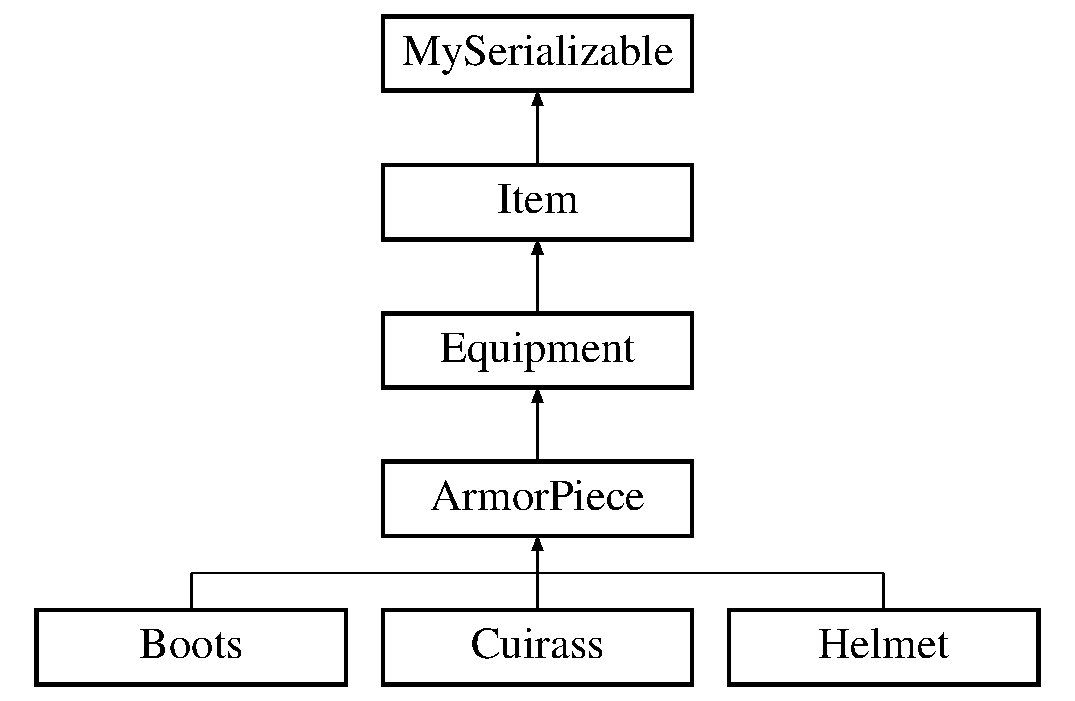
\includegraphics[height=5.000000cm]{class_armor_piece}
\end{center}
\end{figure}
\subsection*{Public Member Functions}
\begin{DoxyCompactItemize}
\item 
\hypertarget{class_armor_piece_a3c4d56ccbd1bb22475cba40c880035bd}{}\label{class_armor_piece_a3c4d56ccbd1bb22475cba40c880035bd} 
int {\bfseries get\+Enchantment} (\hyperlink{class_ability}{Ability} abl)
\item 
\hypertarget{class_armor_piece_a15b22ff2e3958cd099931205382cd1a9}{}\label{class_armor_piece_a15b22ff2e3958cd099931205382cd1a9} 
void {\bfseries set\+Weight} (int new\+Weight)
\item 
\hypertarget{class_armor_piece_a817d88f26d7796118ce4073e716845ab}{}\label{class_armor_piece_a817d88f26d7796118ce4073e716845ab} 
int {\bfseries get\+Weight} ()
\item 
\hypertarget{class_armor_piece_a7069e157bc843765858d5e109879dbc1}{}\label{class_armor_piece_a7069e157bc843765858d5e109879dbc1} 
virtual \hyperlink{class_equip_type}{Equip\+Type} const  $\ast$ {\bfseries get\+Type} ()
\item 
\hypertarget{class_armor_piece_a3de43795bc5a8c7937f69d6200e8a835}{}\label{class_armor_piece_a3de43795bc5a8c7937f69d6200e8a835} 
virtual void {\bfseries save} (std\+::string filename)
\item 
\hypertarget{class_armor_piece_abd9ac9f9b06c808262dea7af7cfca90e}{}\label{class_armor_piece_abd9ac9f9b06c808262dea7af7cfca90e} 
virtual void {\bfseries load} (std\+::string filename)
\end{DoxyCompactItemize}
\subsection*{Protected Member Functions}
\begin{DoxyCompactItemize}
\item 
\hypertarget{class_armor_piece_a7149ebcb6c3cc80666f122981fe460c5}{}\label{class_armor_piece_a7149ebcb6c3cc80666f122981fe460c5} 
{\bfseries Armor\+Piece} (std\+::string a\+Name, \hyperlink{class_equip_type}{Equip\+Type} const $\ast$a\+Type)
\end{DoxyCompactItemize}
\subsection*{Friends}
\begin{DoxyCompactItemize}
\item 
\hypertarget{class_armor_piece_ac98d07dd8f7b70e16ccb9a01abf56b9c}{}\label{class_armor_piece_ac98d07dd8f7b70e16ccb9a01abf56b9c} 
class {\bfseries boost\+::serialization\+::access}
\end{DoxyCompactItemize}


\subsection{Detailed Description}


Definition at line 114 of file inv2.\+h.



The documentation for this class was generated from the following files\+:\begin{DoxyCompactItemize}
\item 
inv2.\+h\item 
inv2.\+cpp\end{DoxyCompactItemize}

\hypertarget{class_belt}{}\section{Belt Class Reference}
\label{class_belt}\index{Belt@{Belt}}
Inheritance diagram for Belt\+:\begin{figure}[H]
\begin{center}
\leavevmode
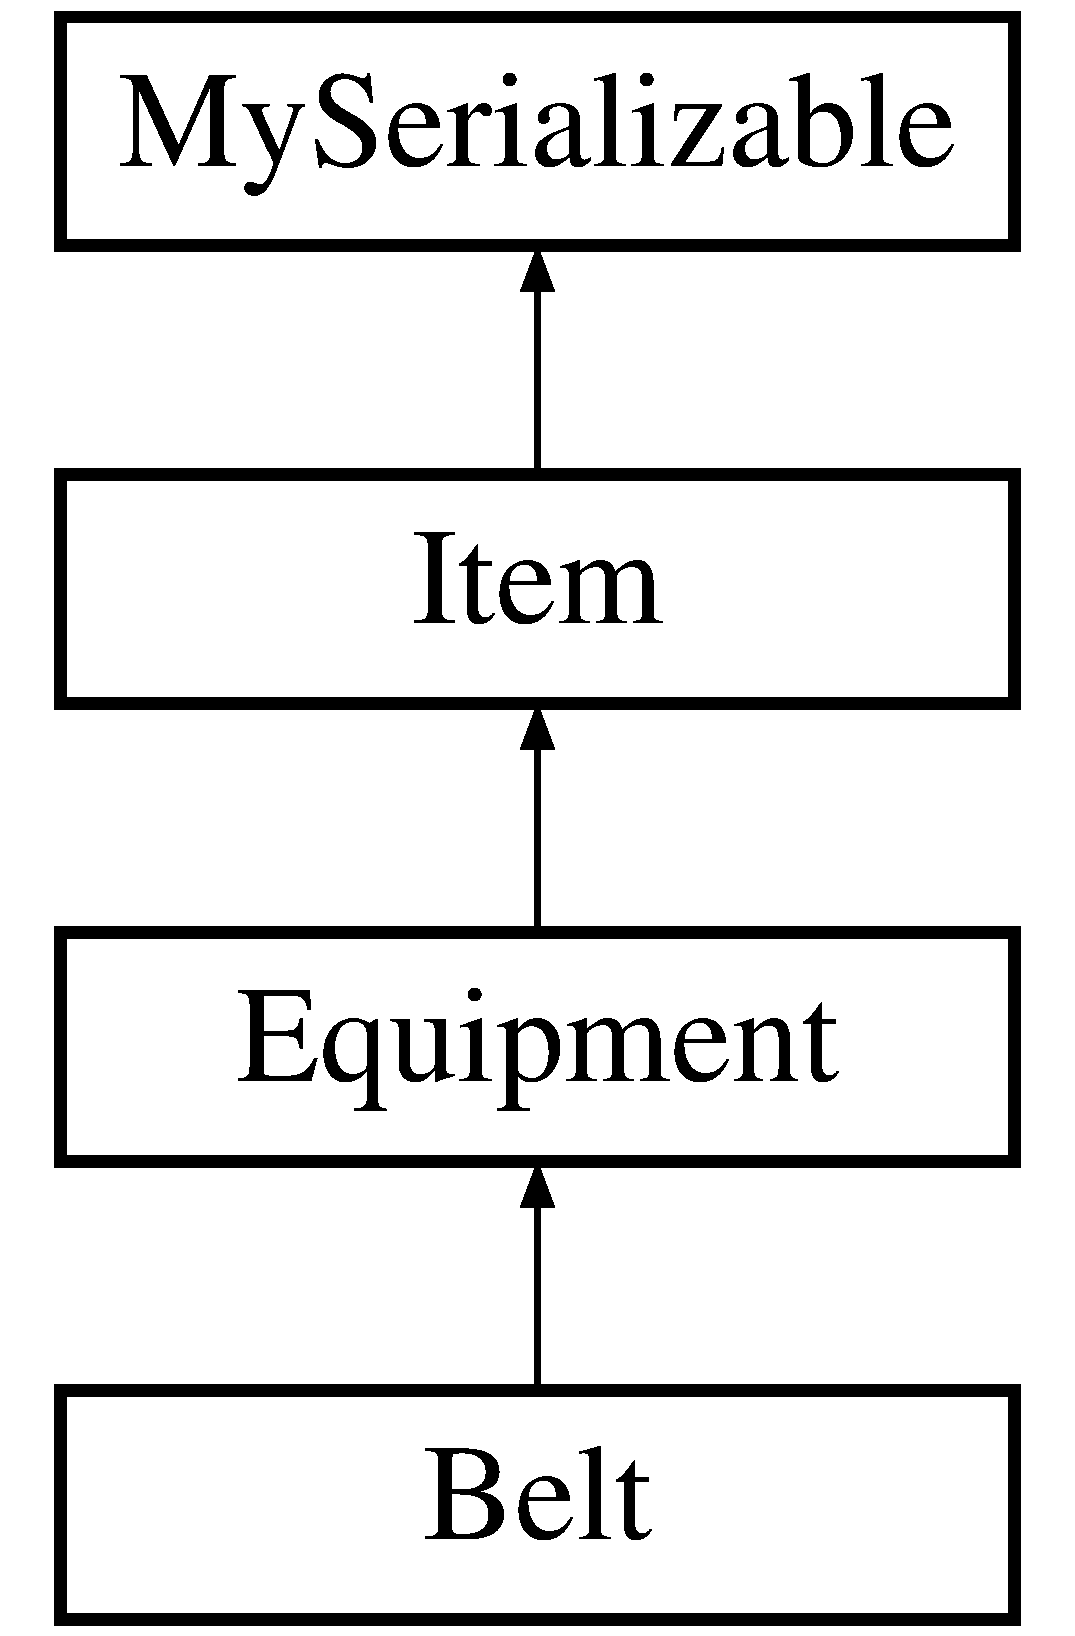
\includegraphics[height=4.000000cm]{class_belt}
\end{center}
\end{figure}
\subsection*{Public Member Functions}
\begin{DoxyCompactItemize}
\item 
\hypertarget{class_belt_a470356c642e72b0f5b802b4fe493db1f}{}\label{class_belt_a470356c642e72b0f5b802b4fe493db1f} 
{\bfseries Belt} (std\+::string a\+Name)
\item 
\hypertarget{class_belt_a03df5b10913866f59261c852326a3e12}{}\label{class_belt_a03df5b10913866f59261c852326a3e12} 
\hyperlink{class_equip_type}{Equip\+Type} const  $\ast$ {\bfseries get\+Type} ()
\item 
\hypertarget{class_belt_a76196f73ef9cd8ddad51461e70635a56}{}\label{class_belt_a76196f73ef9cd8ddad51461e70635a56} 
virtual void {\bfseries save} (std\+::string filename)
\item 
\hypertarget{class_belt_a3e2002db2733fa08c779e12bdc66bd5b}{}\label{class_belt_a3e2002db2733fa08c779e12bdc66bd5b} 
virtual void {\bfseries load} (std\+::string filename)
\end{DoxyCompactItemize}
\subsection*{Static Public Member Functions}
\begin{DoxyCompactItemize}
\item 
\hypertarget{class_belt_a5f1ce1a149d073e7688a6c0d594bf9e8}{}\label{class_belt_a5f1ce1a149d073e7688a6c0d594bf9e8} 
static \hyperlink{class_belt}{Belt} {\bfseries s\+Load} (std\+::string filename)
\end{DoxyCompactItemize}
\subsection*{Friends}
\begin{DoxyCompactItemize}
\item 
\hypertarget{class_belt_ac98d07dd8f7b70e16ccb9a01abf56b9c}{}\label{class_belt_ac98d07dd8f7b70e16ccb9a01abf56b9c} 
class {\bfseries boost\+::serialization\+::access}
\end{DoxyCompactItemize}
\subsection*{Additional Inherited Members}


\subsection{Detailed Description}


Definition at line 219 of file inv2.\+h.



The documentation for this class was generated from the following files\+:\begin{DoxyCompactItemize}
\item 
inv2.\+h\item 
inv2.\+cpp\end{DoxyCompactItemize}

\hypertarget{class_boots}{}\section{Boots Class Reference}
\label{class_boots}\index{Boots@{Boots}}
Inheritance diagram for Boots\+:\begin{figure}[H]
\begin{center}
\leavevmode
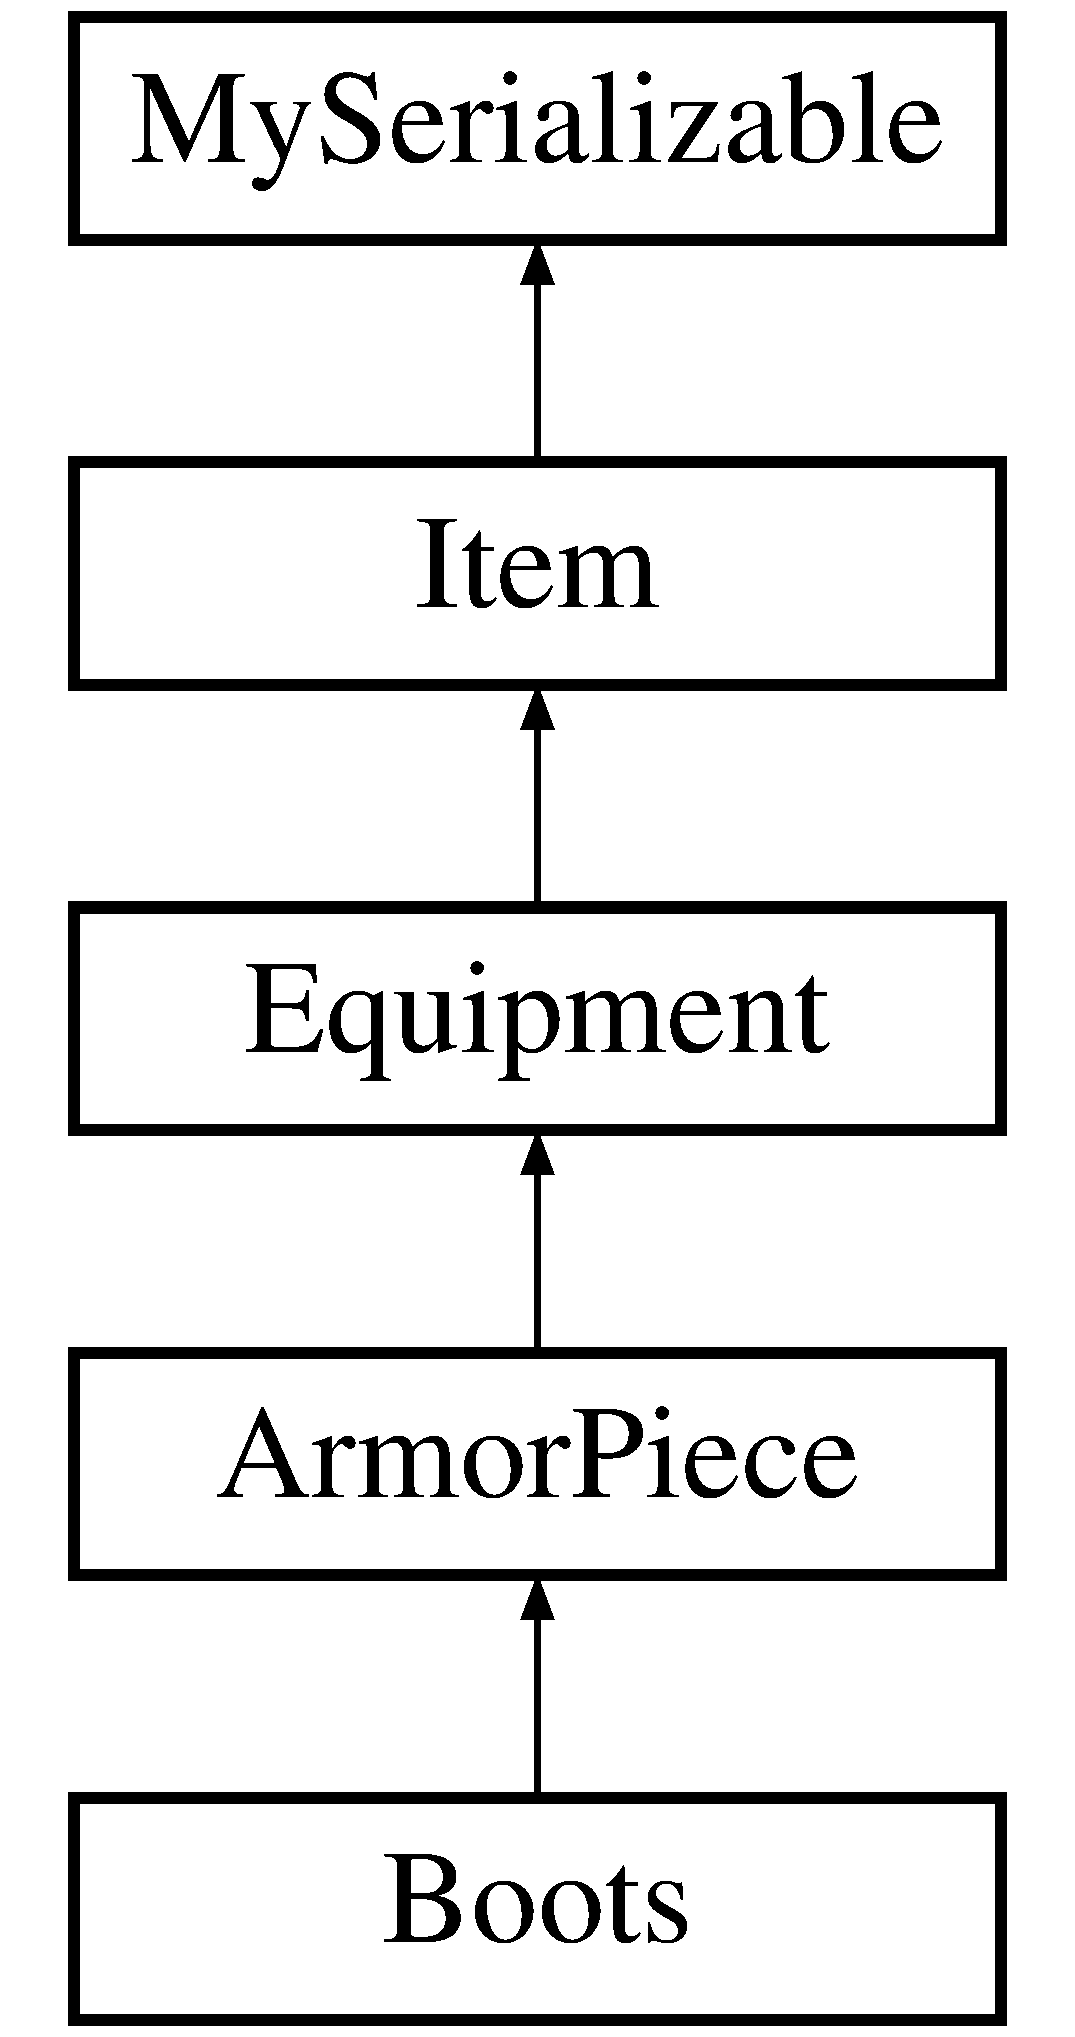
\includegraphics[height=5.000000cm]{class_boots}
\end{center}
\end{figure}
\subsection*{Public Member Functions}
\begin{DoxyCompactItemize}
\item 
\hypertarget{class_boots_a9f8200d7192fb8c315292d8e55146b4a}{}\label{class_boots_a9f8200d7192fb8c315292d8e55146b4a} 
{\bfseries Boots} (std\+::string a\+Name)
\item 
\hypertarget{class_boots_a8c470e56ee8b265014a76320371eadf8}{}\label{class_boots_a8c470e56ee8b265014a76320371eadf8} 
\hyperlink{class_equip_type}{Equip\+Type} const  $\ast$ {\bfseries get\+Type} ()
\item 
\hypertarget{class_boots_a79899d063871ea3d23ff4f3beec91614}{}\label{class_boots_a79899d063871ea3d23ff4f3beec91614} 
virtual void {\bfseries save} (std\+::string filename)
\item 
\hypertarget{class_boots_a4a5857c4ea9d9dedfdc2fc7fe4e6436e}{}\label{class_boots_a4a5857c4ea9d9dedfdc2fc7fe4e6436e} 
virtual void {\bfseries load} (std\+::string filename)
\end{DoxyCompactItemize}
\subsection*{Static Public Member Functions}
\begin{DoxyCompactItemize}
\item 
\hypertarget{class_boots_aaf2b559fc88cb0df3497c02d85d48d24}{}\label{class_boots_aaf2b559fc88cb0df3497c02d85d48d24} 
static \hyperlink{class_boots}{Boots} {\bfseries s\+Load} (std\+::string filename)
\end{DoxyCompactItemize}
\subsection*{Friends}
\begin{DoxyCompactItemize}
\item 
\hypertarget{class_boots_ac98d07dd8f7b70e16ccb9a01abf56b9c}{}\label{class_boots_ac98d07dd8f7b70e16ccb9a01abf56b9c} 
class {\bfseries boost\+::serialization\+::access}
\end{DoxyCompactItemize}
\subsection*{Additional Inherited Members}


\subsection{Detailed Description}


Definition at line 197 of file inv2.\+h.



The documentation for this class was generated from the following files\+:\begin{DoxyCompactItemize}
\item 
inv2.\+h\item 
inv2.\+cpp\end{DoxyCompactItemize}

\hypertarget{class_campain}{}\section{Campain Class Reference}
\label{class_campain}\index{Campain@{Campain}}
\subsection*{Public Member Functions}
\begin{DoxyCompactItemize}
\item 
\hypertarget{class_campain_a40b98ccc22d64dd714be0944970597a8}{}\label{class_campain_a40b98ccc22d64dd714be0944970597a8} 
\hyperlink{class_campain_a40b98ccc22d64dd714be0944970597a8}{Campain} (string new\+Name)
\begin{DoxyCompactList}\small\item\em \hyperlink{class_campain}{Campain} constructor, takes a string name. \end{DoxyCompactList}\item 
\hypertarget{class_campain_ad14dd3cbece20b9737b282fccf4f0ee0}{}\label{class_campain_ad14dd3cbece20b9737b282fccf4f0ee0} 
void \hyperlink{class_campain_ad14dd3cbece20b9737b282fccf4f0ee0}{rename} (string new\+Name)
\begin{DoxyCompactList}\small\item\em \hyperlink{class_campain}{Campain} renaming function. \end{DoxyCompactList}\item 
\hypertarget{class_campain_aa2e22983799e1b99ea554796398c97f1}{}\label{class_campain_aa2e22983799e1b99ea554796398c97f1} 
void \hyperlink{class_campain_aa2e22983799e1b99ea554796398c97f1}{set\+Desc} (string desc)
\begin{DoxyCompactList}\small\item\em \hyperlink{class_campain}{Campain} destructor. \end{DoxyCompactList}\item 
\hypertarget{class_campain_a9d021544799e1555b1f089f3eed95338}{}\label{class_campain_a9d021544799e1555b1f089f3eed95338} 
void {\bfseries add\+Map\+Front} (\hyperlink{class_map}{Map} $\ast$a\+Map)
\item 
\hypertarget{class_campain_aa4a1e6002804d4f75fe985dde1029ae1}{}\label{class_campain_aa4a1e6002804d4f75fe985dde1029ae1} 
void {\bfseries add\+Map\+Back} (\hyperlink{class_map}{Map} $\ast$a\+Map)
\item 
\hypertarget{class_campain_a04709871fad87493c7dc368d18282f61}{}\label{class_campain_a04709871fad87493c7dc368d18282f61} 
void {\bfseries add\+Map\+At} (\hyperlink{class_map}{Map} $\ast$a\+Map, int position)
\item 
\hypertarget{class_campain_abbe7186905f7b9f8e0772af60c78e6f1}{}\label{class_campain_abbe7186905f7b9f8e0772af60c78e6f1} 
void {\bfseries remove\+Map} (\hyperlink{class_map}{Map} $\ast$a\+Map)
\item 
\hypertarget{class_campain_ac6a634b0149cbab03905e352d575e807}{}\label{class_campain_ac6a634b0149cbab03905e352d575e807} 
void {\bfseries remove\+Map} (int position)
\item 
\hypertarget{class_campain_a9e2011c5dc482e3e921d5141ea316cfc}{}\label{class_campain_a9e2011c5dc482e3e921d5141ea316cfc} 
\hyperlink{class_map}{Map} $\ast$ {\bfseries operator\mbox{[}$\,$\mbox{]}} (int i)
\end{DoxyCompactItemize}
\subsection*{Friends}
\begin{DoxyCompactItemize}
\item 
\hypertarget{class_campain_ac98d07dd8f7b70e16ccb9a01abf56b9c}{}\label{class_campain_ac98d07dd8f7b70e16ccb9a01abf56b9c} 
class {\bfseries boost\+::serialization\+::access}
\end{DoxyCompactItemize}


\subsection{Detailed Description}


Definition at line 157 of file map.\+h.



The documentation for this class was generated from the following files\+:\begin{DoxyCompactItemize}
\item 
map.\+h\item 
map.\+cpp\end{DoxyCompactItemize}

\hypertarget{class_cell}{}\section{Cell Class Reference}
\label{class_cell}\index{Cell@{Cell}}
\subsection*{Public Member Functions}
\begin{DoxyCompactItemize}
\item 
\hypertarget{class_cell_a99702fd5fc54b66ffae38a7098c844fd}{}\label{class_cell_a99702fd5fc54b66ffae38a7098c844fd} 
{\bfseries Cell} (int new\+Row, int new\+Col)
\item 
\hypertarget{class_cell_a9fa559f7a28e2b4336c6879ca09304d8}{}\label{class_cell_a9fa559f7a28e2b4336c6879ca09304d8} 
\hyperlink{class_cell_a9fa559f7a28e2b4336c6879ca09304d8}{$\sim$\+Cell} ()
\begin{DoxyCompactList}\small\item\em Board \hyperlink{class_cell}{Cell} destructor. \end{DoxyCompactList}\item 
const int \hyperlink{class_cell_a7d9b27ccd514968a69a2b9ee0ad6c612}{get\+Row} ()
\item 
const int \hyperlink{class_cell_a4c9b2812a2d37e17c1a473e8b905d048}{get\+Col} ()
\item 
std\+::unordered\+\_\+set$<$ \hyperlink{class_cell}{Cell} $\ast$ $>$ \hyperlink{class_cell_a9912ab381441093706286584eff721fa}{get\+Adjacent} ()
\item 
void \hyperlink{class_cell_a90d2e75867bd5f2b553dec1498fdf4e6}{add\+Adjacent} (\hyperlink{class_cell}{Cell} $\ast$a\+Cell)
\item 
void \hyperlink{class_cell_a5d9bda81ac204c982b084c7b02f4d6de}{remove\+Adjacent} (\hyperlink{class_cell}{Cell} $\ast$a\+Cell)
\item 
\hypertarget{class_cell_add026562137122494104071baa175473}{}\label{class_cell_add026562137122494104071baa175473} 
bool \hyperlink{class_cell_add026562137122494104071baa175473}{set\+Content} (\hyperlink{class_placeable}{Placeable} $\ast$new\+Content)
\begin{DoxyCompactList}\small\item\em Function to push \hyperlink{class_placeable}{Placeable} content on a \hyperlink{class_cell}{Cell}. \end{DoxyCompactList}\item 
\hypertarget{class_cell_af1ac11342618275ec6684261e661cb52}{}\label{class_cell_af1ac11342618275ec6684261e661cb52} 
\hyperlink{class_placeable}{Placeable} $\ast$ {\bfseries get\+Content} ()
\item 
\hypertarget{class_cell_a275274592fde050fefcda8515b5a8d3f}{}\label{class_cell_a275274592fde050fefcda8515b5a8d3f} 
void {\bfseries clear} ()
\item 
bool \hyperlink{class_cell_af8625542ca100de4cc6e221ea131f05c}{is\+Walkable} ()
\item 
bool \hyperlink{class_cell_a6c7344ef2aa917e70364221bf86ff8bc}{is\+Empty} ()
\item 
\hypertarget{class_cell_a115541b42cd152e9557d527f6ea3e471}{}\label{class_cell_a115541b42cd152e9557d527f6ea3e471} 
std\+::string {\bfseries to\+String} ()
\end{DoxyCompactItemize}
\subsection*{Static Public Member Functions}
\begin{DoxyCompactItemize}
\item 
\hypertarget{class_cell_ac3a2780a20988ddcfd29aa460dbb7a9e}{}\label{class_cell_ac3a2780a20988ddcfd29aa460dbb7a9e} 
static \hyperlink{class_cell}{Cell} $\ast$ {\bfseries move} (\hyperlink{class_cell}{Cell} $\ast$from, \hyperlink{class_cell}{Cell} $\ast$to)
\end{DoxyCompactItemize}
\subsection*{Friends}
\begin{DoxyCompactItemize}
\item 
\hypertarget{class_cell_ac98d07dd8f7b70e16ccb9a01abf56b9c}{}\label{class_cell_ac98d07dd8f7b70e16ccb9a01abf56b9c} 
class {\bfseries boost\+::serialization\+::access}
\end{DoxyCompactItemize}


\subsection{Detailed Description}


Definition at line 14 of file cell.\+h.



\subsection{Member Function Documentation}
\hypertarget{class_cell_a90d2e75867bd5f2b553dec1498fdf4e6}{}\label{class_cell_a90d2e75867bd5f2b553dec1498fdf4e6} 
\index{Cell@{Cell}!add\+Adjacent@{add\+Adjacent}}
\index{add\+Adjacent@{add\+Adjacent}!Cell@{Cell}}
\subsubsection{\texorpdfstring{add\+Adjacent()}{addAdjacent()}}
{\footnotesize\ttfamily void Cell\+::add\+Adjacent (\begin{DoxyParamCaption}\item[{\hyperlink{class_cell}{Cell} $\ast$}]{a\+Cell }\end{DoxyParamCaption})}

Function to add a cell pointer to the set of adjacent cells. 
\begin{DoxyParams}{Parameters}
{\em a\+Cell} & \hyperlink{class_cell}{Cell} pointer to add to the set of adjacent set. \\
\hline
\end{DoxyParams}


Definition at line 34 of file cell.\+cpp.


\begin{DoxyCode}
35 \{
36     adjacent.insert(aCell);
37 \}
\end{DoxyCode}
\hypertarget{class_cell_a9912ab381441093706286584eff721fa}{}\label{class_cell_a9912ab381441093706286584eff721fa} 
\index{Cell@{Cell}!get\+Adjacent@{get\+Adjacent}}
\index{get\+Adjacent@{get\+Adjacent}!Cell@{Cell}}
\subsubsection{\texorpdfstring{get\+Adjacent()}{getAdjacent()}}
{\footnotesize\ttfamily std\+::unordered\+\_\+set$<$ \hyperlink{class_cell}{Cell} $\ast$ $>$ Cell\+::get\+Adjacent (\begin{DoxyParamCaption}{ }\end{DoxyParamCaption})}

Accessor function for the cell adjacent cells. \begin{DoxyReturn}{Returns}
unordered\+\_\+set of cell pointers to each adjacent cells in the map. 
\end{DoxyReturn}


Definition at line 27 of file cell.\+cpp.


\begin{DoxyCode}
28 \{
29     \textcolor{keywordflow}{return} adjacent;
30 \}
\end{DoxyCode}
\hypertarget{class_cell_a4c9b2812a2d37e17c1a473e8b905d048}{}\label{class_cell_a4c9b2812a2d37e17c1a473e8b905d048} 
\index{Cell@{Cell}!get\+Col@{get\+Col}}
\index{get\+Col@{get\+Col}!Cell@{Cell}}
\subsubsection{\texorpdfstring{get\+Col()}{getCol()}}
{\footnotesize\ttfamily const int Cell\+::get\+Col (\begin{DoxyParamCaption}{ }\end{DoxyParamCaption})}

Accessor function for the cell column. \begin{DoxyReturn}{Returns}
integer of the index of the cell column in its array. 
\end{DoxyReturn}


Definition at line 13 of file cell.\+cpp.


\begin{DoxyCode}
14 \{
15     \textcolor{keywordflow}{return} col;
16 \}
\end{DoxyCode}
\hypertarget{class_cell_a7d9b27ccd514968a69a2b9ee0ad6c612}{}\label{class_cell_a7d9b27ccd514968a69a2b9ee0ad6c612} 
\index{Cell@{Cell}!get\+Row@{get\+Row}}
\index{get\+Row@{get\+Row}!Cell@{Cell}}
\subsubsection{\texorpdfstring{get\+Row()}{getRow()}}
{\footnotesize\ttfamily const int Cell\+::get\+Row (\begin{DoxyParamCaption}{ }\end{DoxyParamCaption})}

Accessor function for the cell row. \begin{DoxyReturn}{Returns}
integer of the index of the cell row in its array. 
\end{DoxyReturn}


Definition at line 20 of file cell.\+cpp.


\begin{DoxyCode}
21 \{
22     \textcolor{keywordflow}{return} row;
23 \}
\end{DoxyCode}
\hypertarget{class_cell_a6c7344ef2aa917e70364221bf86ff8bc}{}\label{class_cell_a6c7344ef2aa917e70364221bf86ff8bc} 
\index{Cell@{Cell}!is\+Empty@{is\+Empty}}
\index{is\+Empty@{is\+Empty}!Cell@{Cell}}
\subsubsection{\texorpdfstring{is\+Empty()}{isEmpty()}}
{\footnotesize\ttfamily bool Cell\+::is\+Empty (\begin{DoxyParamCaption}{ }\end{DoxyParamCaption})}

Function to check if the cell holds some content or not. \begin{DoxyReturn}{Returns}
bool value, true if the cell\textquotesingle{}s \hyperlink{class_placeable}{Placeable} pointer is null. 
\end{DoxyReturn}


Definition at line 71 of file cell.\+cpp.


\begin{DoxyCode}
72 \{
73     \textcolor{keywordflow}{return} (content == NULL);
74 \}
\end{DoxyCode}
\hypertarget{class_cell_af8625542ca100de4cc6e221ea131f05c}{}\label{class_cell_af8625542ca100de4cc6e221ea131f05c} 
\index{Cell@{Cell}!is\+Walkable@{is\+Walkable}}
\index{is\+Walkable@{is\+Walkable}!Cell@{Cell}}
\subsubsection{\texorpdfstring{is\+Walkable()}{isWalkable()}}
{\footnotesize\ttfamily bool Cell\+::is\+Walkable (\begin{DoxyParamCaption}{ }\end{DoxyParamCaption})}

Function to check if the cell blocks a path or not. \begin{DoxyReturn}{Returns}
bool value, true if the cell\textquotesingle{}s Cell\+Content pointer is null Or if it is walkable. 
\end{DoxyReturn}


Definition at line 62 of file cell.\+cpp.


\begin{DoxyCode}
63 \{
64     \textcolor{keywordflow}{if} (content == NULL) \textcolor{keywordflow}{return} \textcolor{keyword}{true};
65     
66     \textcolor{keywordflow}{return} content->isWalkable();
67 \}
\end{DoxyCode}
\hypertarget{class_cell_a5d9bda81ac204c982b084c7b02f4d6de}{}\label{class_cell_a5d9bda81ac204c982b084c7b02f4d6de} 
\index{Cell@{Cell}!remove\+Adjacent@{remove\+Adjacent}}
\index{remove\+Adjacent@{remove\+Adjacent}!Cell@{Cell}}
\subsubsection{\texorpdfstring{remove\+Adjacent()}{removeAdjacent()}}
{\footnotesize\ttfamily void Cell\+::remove\+Adjacent (\begin{DoxyParamCaption}\item[{\hyperlink{class_cell}{Cell} $\ast$}]{a\+Cell }\end{DoxyParamCaption})}

Function to remove a cell pointer to the set of adjacent cells. 
\begin{DoxyParams}{Parameters}
{\em a\+Cell} & \hyperlink{class_cell}{Cell} pointer to remove from the set of adjacent cells. \\
\hline
\end{DoxyParams}


Definition at line 41 of file cell.\+cpp.


\begin{DoxyCode}
42 \{
43     adjacent.erase(aCell);
44 \}
\end{DoxyCode}


The documentation for this class was generated from the following files\+:\begin{DoxyCompactItemize}
\item 
cell.\+h\item 
cell.\+cpp\end{DoxyCompactItemize}

\hypertarget{class_cell_list}{}\section{Cell\+List Class Reference}
\label{class_cell_list}\index{Cell\+List@{Cell\+List}}
\subsection*{Public Member Functions}
\begin{DoxyCompactItemize}
\item 
\hypertarget{class_cell_list_aa5c3ce5f60d54a1222f783b719f7f18d}{}\label{class_cell_list_aa5c3ce5f60d54a1222f783b719f7f18d} 
\hyperlink{class_cell_list_aa5c3ce5f60d54a1222f783b719f7f18d}{Cell\+List} ()
\begin{DoxyCompactList}\small\item\em Default constructor of a \hyperlink{class_cell_list}{Cell\+List} object. \end{DoxyCompactList}\item 
\hypertarget{class_cell_list_a2f7854cd49caefac1f84654ab550e896}{}\label{class_cell_list_a2f7854cd49caefac1f84654ab550e896} 
\hyperlink{class_cell_list_a2f7854cd49caefac1f84654ab550e896}{$\sim$\+Cell\+List} ()
\begin{DoxyCompactList}\small\item\em Default \hyperlink{class_cell_list}{Cell\+List} destructor. \end{DoxyCompactList}\item 
std\+::list$<$ \hyperlink{class_cell}{Cell} $\ast$ $>$ \hyperlink{class_cell_list_aa5fee7de166143e16a0ec1f20349db55}{get\+List} ()
\begin{DoxyCompactList}\small\item\em Accessor function to cell\+\_\+list. \end{DoxyCompactList}\item 
void \hyperlink{class_cell_list_a94857958e9f2156c7b4c76fd774a5fda}{add\+All} (std\+::unordered\+\_\+set$<$ \hyperlink{class_cell}{Cell} $\ast$$>$ a\+Set)
\begin{DoxyCompactList}\small\item\em Function to add all of a set elements to cell\+\_\+list. \end{DoxyCompactList}\item 
\hyperlink{class_cell}{Cell} $\ast$ \hyperlink{class_cell_list_abc7337272382af9d9782628666f9e594}{remove} ()
\begin{DoxyCompactList}\small\item\em Function that removes and returns the first element of the List cell\+\_\+list. \end{DoxyCompactList}\item 
bool \hyperlink{class_cell_list_a5df3e74d57494b51859a6a223f8b2a30}{empty} ()
\begin{DoxyCompactList}\small\item\em Asserts if cell\+\_\+list is empty. \end{DoxyCompactList}\end{DoxyCompactItemize}


\subsection{Detailed Description}


Definition at line 152 of file map.\+h.



\subsection{Member Function Documentation}
\hypertarget{class_cell_list_a94857958e9f2156c7b4c76fd774a5fda}{}\label{class_cell_list_a94857958e9f2156c7b4c76fd774a5fda} 
\index{Cell\+List@{Cell\+List}!add\+All@{add\+All}}
\index{add\+All@{add\+All}!Cell\+List@{Cell\+List}}
\subsubsection{\texorpdfstring{add\+All()}{addAll()}}
{\footnotesize\ttfamily void Cell\+List\+::add\+All (\begin{DoxyParamCaption}\item[{std\+::unordered\+\_\+set$<$ \hyperlink{class_cell}{Cell} $\ast$$>$}]{a\+Set }\end{DoxyParamCaption})}



Function to add all of a set elements to cell\+\_\+list. 


\begin{DoxyParams}{Parameters}
{\em a\+Set} & and Unordered\+\_\+set of \hyperlink{class_cell}{Cell} pointers to add to the List cell\+\_\+list. \\
\hline
\end{DoxyParams}


Definition at line 722 of file map.\+cpp.


\begin{DoxyCode}
723 \{
724     \textcolor{keywordflow}{for}(\hyperlink{class_cell}{Cell}* c: aSet)
725     \{
726         cell\_list.push\_front(c);
727     \}
728 \}
\end{DoxyCode}
\hypertarget{class_cell_list_a5df3e74d57494b51859a6a223f8b2a30}{}\label{class_cell_list_a5df3e74d57494b51859a6a223f8b2a30} 
\index{Cell\+List@{Cell\+List}!empty@{empty}}
\index{empty@{empty}!Cell\+List@{Cell\+List}}
\subsubsection{\texorpdfstring{empty()}{empty()}}
{\footnotesize\ttfamily bool Cell\+List\+::empty (\begin{DoxyParamCaption}{ }\end{DoxyParamCaption})}



Asserts if cell\+\_\+list is empty. 

return true if the \hyperlink{class_cell}{Cell} pointer List cell\+\_\+list contains no elements. 

Definition at line 741 of file map.\+cpp.


\begin{DoxyCode}
742 \{
743     \textcolor{keywordflow}{return} cell\_list.empty();
744 \}
\end{DoxyCode}
\hypertarget{class_cell_list_aa5fee7de166143e16a0ec1f20349db55}{}\label{class_cell_list_aa5fee7de166143e16a0ec1f20349db55} 
\index{Cell\+List@{Cell\+List}!get\+List@{get\+List}}
\index{get\+List@{get\+List}!Cell\+List@{Cell\+List}}
\subsubsection{\texorpdfstring{get\+List()}{getList()}}
{\footnotesize\ttfamily std\+::list$<$ \hyperlink{class_cell}{Cell} $\ast$ $>$ Cell\+List\+::get\+List (\begin{DoxyParamCaption}{ }\end{DoxyParamCaption})}



Accessor function to cell\+\_\+list. 

return the list of \hyperlink{class_cell}{Cell} pointers cell\+\_\+list. 

Definition at line 715 of file map.\+cpp.


\begin{DoxyCode}
716 \{
717     \textcolor{keywordflow}{return} cell\_list;
718 \}
\end{DoxyCode}
\hypertarget{class_cell_list_abc7337272382af9d9782628666f9e594}{}\label{class_cell_list_abc7337272382af9d9782628666f9e594} 
\index{Cell\+List@{Cell\+List}!remove@{remove}}
\index{remove@{remove}!Cell\+List@{Cell\+List}}
\subsubsection{\texorpdfstring{remove()}{remove()}}
{\footnotesize\ttfamily \hyperlink{class_cell}{Cell} $\ast$ Cell\+List\+::remove (\begin{DoxyParamCaption}{ }\end{DoxyParamCaption})}



Function that removes and returns the first element of the List cell\+\_\+list. 

\begin{DoxyReturn}{Returns}
\hyperlink{class_cell}{Cell} pointer, first element of the \hyperlink{class_cell}{Cell} pointer list cell\+\_\+list. 
\end{DoxyReturn}


Definition at line 732 of file map.\+cpp.


\begin{DoxyCode}
733 \{
734     \hyperlink{class_cell}{Cell}* c = cell\_list.front();
735     cell\_list.pop\_front();
736     \textcolor{keywordflow}{return} c;
737 \}
\end{DoxyCode}


The documentation for this class was generated from the following files\+:\begin{DoxyCompactItemize}
\item 
map.\+h\item 
map.\+cpp\end{DoxyCompactItemize}

\hypertarget{class_cell_set}{}\section{Cell\+Set Class Reference}
\label{class_cell_set}\index{Cell\+Set@{Cell\+Set}}
\subsection*{Public Member Functions}
\begin{DoxyCompactItemize}
\item 
\hypertarget{class_cell_set_a0f0e0b518cd5fd70c0e1841e3df6eff9}{}\label{class_cell_set_a0f0e0b518cd5fd70c0e1841e3df6eff9} 
\hyperlink{class_cell_set_a0f0e0b518cd5fd70c0e1841e3df6eff9}{Cell\+Set} ()
\begin{DoxyCompactList}\small\item\em Default constructor of a \hyperlink{class_cell_set}{Cell\+Set} object. \end{DoxyCompactList}\item 
\hypertarget{class_cell_set_a6e9f853835e8982dd178dad534a9678c}{}\label{class_cell_set_a6e9f853835e8982dd178dad534a9678c} 
\hyperlink{class_cell_set_a6e9f853835e8982dd178dad534a9678c}{$\sim$\+Cell\+Set} ()
\begin{DoxyCompactList}\small\item\em Default \hyperlink{class_cell_set}{Cell\+Set} destructor. \end{DoxyCompactList}\item 
std\+::unordered\+\_\+set$<$ \hyperlink{class_cell}{Cell} $\ast$ $>$ \hyperlink{class_cell_set_a16ffb9da795fb77b5214ff0ad276c325}{get\+Set} ()
\begin{DoxyCompactList}\small\item\em Accessor function to cell\+\_\+set. \end{DoxyCompactList}\item 
void \hyperlink{class_cell_set_a589f95793822a6c76b45ab3c5cadeda3}{insert} (\hyperlink{class_cell}{Cell} $\ast$a\+Cell)
\begin{DoxyCompactList}\small\item\em Function to that inserts a \hyperlink{class_cell}{Cell} pointer in cell\+\_\+set. \end{DoxyCompactList}\item 
void \hyperlink{class_cell_set_a9e802e2d27938d62d578bdf602e540c3}{add\+All} (std\+::unordered\+\_\+set$<$ \hyperlink{class_cell}{Cell} $\ast$$>$ a\+Set)
\begin{DoxyCompactList}\small\item\em Function to add all of a \hyperlink{class_cell}{Cell} pointer set elements to cell\+\_\+set. \end{DoxyCompactList}\item 
void \hyperlink{class_cell_set_a0d3c7fe4074fff58db2bf6932bf20ab0}{add\+All} (std\+::list$<$ \hyperlink{class_cell}{Cell} $\ast$$>$ a\+List)
\begin{DoxyCompactList}\small\item\em Function to add all of a \hyperlink{class_cell}{Cell} pointer list elements to cell\+\_\+set. \end{DoxyCompactList}\item 
void \hyperlink{class_cell_set_a13671e16ec2d31a9d5ae628f0df87890}{remove\+All} (std\+::unordered\+\_\+set$<$ \hyperlink{class_cell}{Cell} $\ast$$>$ a\+Set)
\begin{DoxyCompactList}\small\item\em Function to remove all of a \hyperlink{class_cell}{Cell} pointer Unordered\+\_\+set elements present in cell\+\_\+set. \end{DoxyCompactList}\item 
bool \hyperlink{class_cell_set_aaf42eb737301463a3ebf6a86c13a7dc4}{empty} ()
\begin{DoxyCompactList}\small\item\em Asserts if cell\+\_\+set is empty. \end{DoxyCompactList}\end{DoxyCompactItemize}


\subsection{Detailed Description}


Definition at line 141 of file map.\+h.



\subsection{Member Function Documentation}
\hypertarget{class_cell_set_a9e802e2d27938d62d578bdf602e540c3}{}\label{class_cell_set_a9e802e2d27938d62d578bdf602e540c3} 
\index{Cell\+Set@{Cell\+Set}!add\+All@{add\+All}}
\index{add\+All@{add\+All}!Cell\+Set@{Cell\+Set}}
\subsubsection{\texorpdfstring{add\+All()}{addAll()}\hspace{0.1cm}{\footnotesize\ttfamily [1/2]}}
{\footnotesize\ttfamily void Cell\+Set\+::add\+All (\begin{DoxyParamCaption}\item[{std\+::unordered\+\_\+set$<$ \hyperlink{class_cell}{Cell} $\ast$$>$}]{a\+Set }\end{DoxyParamCaption})}



Function to add all of a \hyperlink{class_cell}{Cell} pointer set elements to cell\+\_\+set. 


\begin{DoxyParams}{Parameters}
{\em a\+Set} & an Unordered\+\_\+set of \hyperlink{class_cell}{Cell} pointers to add to the Unordered\+\_\+set cell\+\_\+set. \\
\hline
\end{DoxyParams}


Definition at line 603 of file map.\+cpp.


\begin{DoxyCode}
604 \{
605     \textcolor{keywordflow}{for} (\hyperlink{class_cell}{Cell}* c: aSet)
606     \{
607         cell\_set.insert(c);
608     \}
609 \}
\end{DoxyCode}
\hypertarget{class_cell_set_a0d3c7fe4074fff58db2bf6932bf20ab0}{}\label{class_cell_set_a0d3c7fe4074fff58db2bf6932bf20ab0} 
\index{Cell\+Set@{Cell\+Set}!add\+All@{add\+All}}
\index{add\+All@{add\+All}!Cell\+Set@{Cell\+Set}}
\subsubsection{\texorpdfstring{add\+All()}{addAll()}\hspace{0.1cm}{\footnotesize\ttfamily [2/2]}}
{\footnotesize\ttfamily void Cell\+Set\+::add\+All (\begin{DoxyParamCaption}\item[{std\+::list$<$ \hyperlink{class_cell}{Cell} $\ast$$>$}]{a\+List }\end{DoxyParamCaption})}



Function to add all of a \hyperlink{class_cell}{Cell} pointer list elements to cell\+\_\+set. 


\begin{DoxyParams}{Parameters}
{\em a\+Set} & a List of \hyperlink{class_cell}{Cell} pointers to add to the Unordered\+\_\+set cell\+\_\+set. \\
\hline
\end{DoxyParams}


Definition at line 613 of file map.\+cpp.


\begin{DoxyCode}
614 \{
615     \textcolor{keywordflow}{for} (\hyperlink{class_cell}{Cell}* c: aList)
616     \{
617         cell\_set.insert(c);
618     \}
619 \}
\end{DoxyCode}
\hypertarget{class_cell_set_aaf42eb737301463a3ebf6a86c13a7dc4}{}\label{class_cell_set_aaf42eb737301463a3ebf6a86c13a7dc4} 
\index{Cell\+Set@{Cell\+Set}!empty@{empty}}
\index{empty@{empty}!Cell\+Set@{Cell\+Set}}
\subsubsection{\texorpdfstring{empty()}{empty()}}
{\footnotesize\ttfamily bool Cell\+Set\+::empty (\begin{DoxyParamCaption}{ }\end{DoxyParamCaption})}



Asserts if cell\+\_\+set is empty. 

return true if the \hyperlink{class_cell}{Cell} pointer Unordered\+\_\+set cell\+\_\+set contains no elements. 

Definition at line 632 of file map.\+cpp.


\begin{DoxyCode}
633 \{
634     \textcolor{keywordflow}{return} cell\_set.empty();
635 \}
\end{DoxyCode}
\hypertarget{class_cell_set_a16ffb9da795fb77b5214ff0ad276c325}{}\label{class_cell_set_a16ffb9da795fb77b5214ff0ad276c325} 
\index{Cell\+Set@{Cell\+Set}!get\+Set@{get\+Set}}
\index{get\+Set@{get\+Set}!Cell\+Set@{Cell\+Set}}
\subsubsection{\texorpdfstring{get\+Set()}{getSet()}}
{\footnotesize\ttfamily std\+::unordered\+\_\+set$<$ \hyperlink{class_cell}{Cell} $\ast$ $>$ Cell\+Set\+::get\+Set (\begin{DoxyParamCaption}{ }\end{DoxyParamCaption})}



Accessor function to cell\+\_\+set. 

return the Unordered\+\_\+set of \hyperlink{class_cell}{Cell} pointers cell\+\_\+set. 

Definition at line 589 of file map.\+cpp.


\begin{DoxyCode}
590 \{
591     \textcolor{keywordflow}{return} cell\_set;
592 \}
\end{DoxyCode}
\hypertarget{class_cell_set_a589f95793822a6c76b45ab3c5cadeda3}{}\label{class_cell_set_a589f95793822a6c76b45ab3c5cadeda3} 
\index{Cell\+Set@{Cell\+Set}!insert@{insert}}
\index{insert@{insert}!Cell\+Set@{Cell\+Set}}
\subsubsection{\texorpdfstring{insert()}{insert()}}
{\footnotesize\ttfamily void Cell\+Set\+::insert (\begin{DoxyParamCaption}\item[{\hyperlink{class_cell}{Cell} $\ast$}]{a\+Cell }\end{DoxyParamCaption})}



Function to that inserts a \hyperlink{class_cell}{Cell} pointer in cell\+\_\+set. 


\begin{DoxyParams}{Parameters}
{\em a\+Cell} & \hyperlink{class_cell}{Cell} pointer to insert in the Unordered\+\_\+set cell\+\_\+set. \\
\hline
\end{DoxyParams}


Definition at line 596 of file map.\+cpp.


\begin{DoxyCode}
597 \{
598     cell\_set.insert(aCell);
599 \}
\end{DoxyCode}
\hypertarget{class_cell_set_a13671e16ec2d31a9d5ae628f0df87890}{}\label{class_cell_set_a13671e16ec2d31a9d5ae628f0df87890} 
\index{Cell\+Set@{Cell\+Set}!remove\+All@{remove\+All}}
\index{remove\+All@{remove\+All}!Cell\+Set@{Cell\+Set}}
\subsubsection{\texorpdfstring{remove\+All()}{removeAll()}}
{\footnotesize\ttfamily void Cell\+Set\+::remove\+All (\begin{DoxyParamCaption}\item[{std\+::unordered\+\_\+set$<$ \hyperlink{class_cell}{Cell} $\ast$$>$}]{a\+Set }\end{DoxyParamCaption})}



Function to remove all of a \hyperlink{class_cell}{Cell} pointer Unordered\+\_\+set elements present in cell\+\_\+set. 


\begin{DoxyParams}{Parameters}
{\em a\+Set} & an Unordered\+\_\+set of \hyperlink{class_cell}{Cell} pointers to remove to the Unordered\+\_\+set cell\+\_\+set. \\
\hline
\end{DoxyParams}


Definition at line 623 of file map.\+cpp.


\begin{DoxyCode}
624 \{
625     \textcolor{keywordflow}{for} (\hyperlink{class_cell}{Cell}* c : aSet)
626     \{
627         cell\_set.erase(c);
628     \}
629 \}
\end{DoxyCode}


The documentation for this class was generated from the following files\+:\begin{DoxyCompactItemize}
\item 
map.\+h\item 
map.\+cpp\end{DoxyCompactItemize}

\hypertarget{class_chest}{}\section{Chest Class Reference}
\label{class_chest}\index{Chest@{Chest}}
Inheritance diagram for Chest\+:\begin{figure}[H]
\begin{center}
\leavevmode
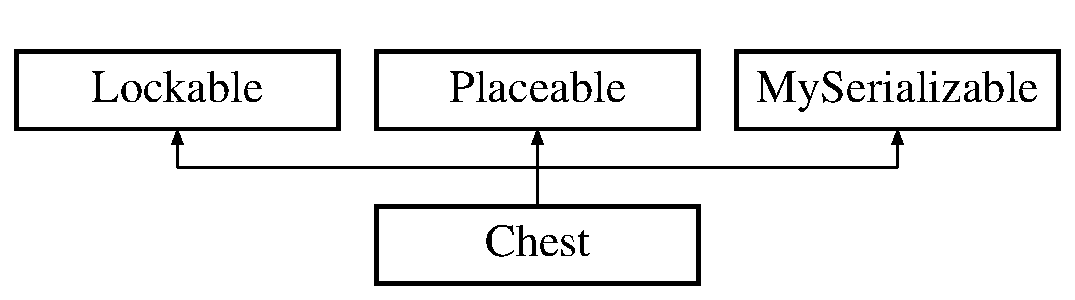
\includegraphics[height=2.000000cm]{class_chest}
\end{center}
\end{figure}
\subsection*{Public Member Functions}
\begin{DoxyCompactItemize}
\item 
\hypertarget{class_chest_a42b87228cbd720ca3e6bbe54a72cd3ee}{}\label{class_chest_a42b87228cbd720ca3e6bbe54a72cd3ee} 
const char {\bfseries get\+Symbol} ()
\item 
\hypertarget{class_chest_aa6c95831a0e55155c917323f7bd24249}{}\label{class_chest_aa6c95831a0e55155c917323f7bd24249} 
void {\bfseries update\+Lvl} (int a\+Level)
\item 
\hypertarget{class_chest_ac14bf4adcd35db79f8cd018aaffb2bab}{}\label{class_chest_ac14bf4adcd35db79f8cd018aaffb2bab} 
bool {\bfseries reset} ()
\item 
\hypertarget{class_chest_a2ae8e14e58fb1b50214935057b7cb103}{}\label{class_chest_a2ae8e14e58fb1b50214935057b7cb103} 
bool {\bfseries open} (\hyperlink{class_key_item}{Key\+Item} $\ast$a\+Key)
\item 
\hypertarget{class_chest_a6bed6abc28230857fae972d1502e4439}{}\label{class_chest_a6bed6abc28230857fae972d1502e4439} 
bool {\bfseries add\+Item} (\hyperlink{class_item}{Item} $\ast$an\+Item)
\item 
\hypertarget{class_chest_a72987b964c8616fdc74344a9d9f8d095}{}\label{class_chest_a72987b964c8616fdc74344a9d9f8d095} 
void {\bfseries remove\+Item} (\hyperlink{class_item}{Item} $\ast$an\+Item)
\item 
\hypertarget{class_chest_ae4663c7ab039a1a13a39c1c9ab7e3ac9}{}\label{class_chest_ae4663c7ab039a1a13a39c1c9ab7e3ac9} 
unordered\+\_\+set$<$ \hyperlink{class_item}{Item} $\ast$ $>$ {\bfseries get\+All} ()
\item 
\hypertarget{class_chest_a0a3e28a480606f1a650a34043992f880}{}\label{class_chest_a0a3e28a480606f1a650a34043992f880} 
unordered\+\_\+set$<$ \hyperlink{class_item}{Item} $\ast$ $>$ {\bfseries remove\+All} ()
\item 
\hypertarget{class_chest_a0a10f9b5a9ec421f6f3756b39edc92b9}{}\label{class_chest_a0a10f9b5a9ec421f6f3756b39edc92b9} 
std\+::string {\bfseries key\+Name} ()
\item 
\hypertarget{class_chest_a263bdda01679de8aa3fef71036d33b2a}{}\label{class_chest_a263bdda01679de8aa3fef71036d33b2a} 
bool {\bfseries is\+Walkable} ()
\item 
\hypertarget{class_chest_a956e975682338b63e5f51b975c9707d4}{}\label{class_chest_a956e975682338b63e5f51b975c9707d4} 
void {\bfseries load} (std\+::string filename)
\item 
\hypertarget{class_chest_a0a0077543c751d68acd1130845561559}{}\label{class_chest_a0a0077543c751d68acd1130845561559} 
void {\bfseries save} (std\+::string filename)
\item 
\hypertarget{class_chest_a54b773b175e8961c0dca87409a96507b}{}\label{class_chest_a54b773b175e8961c0dca87409a96507b} 
std\+::string {\bfseries to\+String} ()
\end{DoxyCompactItemize}
\subsection*{Static Public Member Functions}
\begin{DoxyCompactItemize}
\item 
\hypertarget{class_chest_a577f83d173be0331b92093dcfb2cf4ca}{}\label{class_chest_a577f83d173be0331b92093dcfb2cf4ca} 
static \hyperlink{class_chest}{Chest} {\bfseries s\+Load} (std\+::string filename)
\end{DoxyCompactItemize}
\subsection*{Friends}
\begin{DoxyCompactItemize}
\item 
\hypertarget{class_chest_ac98d07dd8f7b70e16ccb9a01abf56b9c}{}\label{class_chest_ac98d07dd8f7b70e16ccb9a01abf56b9c} 
class {\bfseries boost\+::serialization\+::access}
\end{DoxyCompactItemize}
\subsection*{Additional Inherited Members}


\subsection{Detailed Description}


Definition at line 88 of file basic\+\_\+structure.\+h.



The documentation for this class was generated from the following files\+:\begin{DoxyCompactItemize}
\item 
basic\+\_\+structure.\+h\item 
basic\+\_\+structure.\+cpp\end{DoxyCompactItemize}

\hypertarget{class_cuirass}{}\section{Cuirass Class Reference}
\label{class_cuirass}\index{Cuirass@{Cuirass}}


{\ttfamily \#include $<$inv2.\+h$>$}

Inheritance diagram for Cuirass\+:\begin{figure}[H]
\begin{center}
\leavevmode
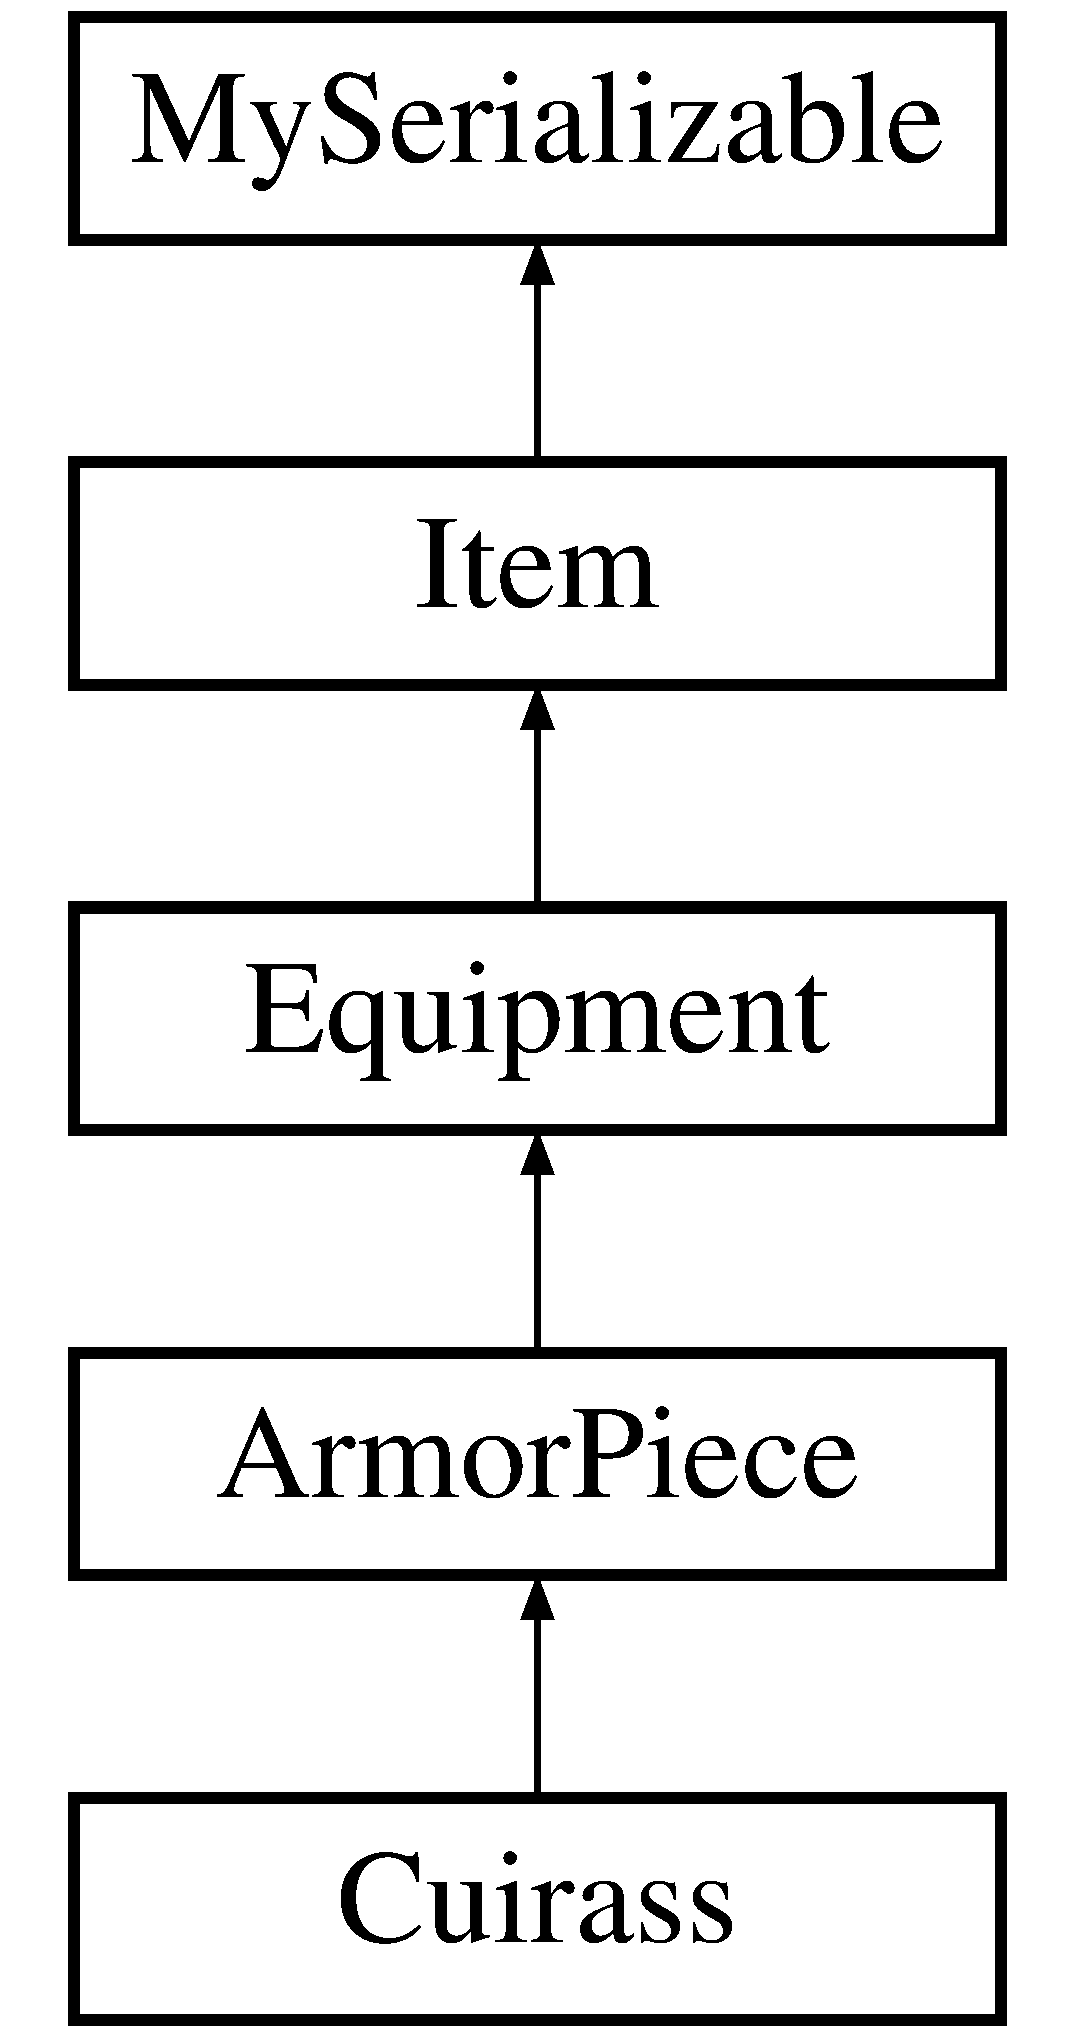
\includegraphics[height=5.000000cm]{class_cuirass}
\end{center}
\end{figure}
\subsection*{Public Member Functions}
\begin{DoxyCompactItemize}
\item 
\hypertarget{class_cuirass_a4fe284b22f6d10ab28098eac7b65ed41}{}\label{class_cuirass_a4fe284b22f6d10ab28098eac7b65ed41} 
{\bfseries Cuirass} (std\+::string a\+Name)
\item 
\hypertarget{class_cuirass_a214e66939642605ab737c5e92d72e1a2}{}\label{class_cuirass_a214e66939642605ab737c5e92d72e1a2} 
\hyperlink{class_equip_type}{Equip\+Type} const  $\ast$ {\bfseries get\+Type} ()
\item 
\hypertarget{class_cuirass_ad181561b5972934e1dcf12c9341b47a3}{}\label{class_cuirass_ad181561b5972934e1dcf12c9341b47a3} 
virtual void {\bfseries save} (std\+::string filename)
\item 
\hypertarget{class_cuirass_a94f018c99f660943107f77ddeff43e03}{}\label{class_cuirass_a94f018c99f660943107f77ddeff43e03} 
virtual void {\bfseries load} (std\+::string filename)
\end{DoxyCompactItemize}
\subsection*{Static Public Member Functions}
\begin{DoxyCompactItemize}
\item 
\hypertarget{class_cuirass_aabc3b7ab1486d7714a0b7a4f412a41e9}{}\label{class_cuirass_aabc3b7ab1486d7714a0b7a4f412a41e9} 
static \hyperlink{class_cuirass}{Cuirass} {\bfseries s\+Load} (std\+::string filename)
\end{DoxyCompactItemize}
\subsection*{Friends}
\begin{DoxyCompactItemize}
\item 
\hypertarget{class_cuirass_ac98d07dd8f7b70e16ccb9a01abf56b9c}{}\label{class_cuirass_ac98d07dd8f7b70e16ccb9a01abf56b9c} 
class {\bfseries boost\+::serialization\+::access}
\end{DoxyCompactItemize}
\subsection*{Additional Inherited Members}


\subsection{Detailed Description}
Class for the main body protection \hyperlink{class_equip_type}{Equip\+Type}. Derives Armor\+Type. 

Definition at line 176 of file inv2.\+h.



The documentation for this class was generated from the following files\+:\begin{DoxyCompactItemize}
\item 
inv2.\+h\item 
inv2.\+cpp\end{DoxyCompactItemize}

\hypertarget{class_dice}{}\section{Dice Class Reference}
\label{class_dice}\index{Dice@{Dice}}
\subsection*{Static Public Member Functions}
\begin{DoxyCompactItemize}
\item 
\hypertarget{class_dice_ac94cb9c94fccfc5579310769b39056a6}{}\label{class_dice_ac94cb9c94fccfc5579310769b39056a6} 
static int \hyperlink{class_dice_ac94cb9c94fccfc5579310769b39056a6}{roll} (const int nbr\+\_\+dice, const int faces)
\begin{DoxyCompactList}\small\item\em dice method. \end{DoxyCompactList}\item 
\hypertarget{class_dice_a1b9a9c31860b6e8b980ea5e3bf4494cd}{}\label{class_dice_a1b9a9c31860b6e8b980ea5e3bf4494cd} 
static int {\bfseries roll} (const int nbr\+\_\+dice, const int faces, const int modifier)
\item 
\hypertarget{class_dice_a8ad5ba0b908fba18df7c0e8795fc55fb}{}\label{class_dice_a8ad5ba0b908fba18df7c0e8795fc55fb} 
static int {\bfseries ability\+Roll} ()
\end{DoxyCompactItemize}


\subsection{Detailed Description}


Definition at line 109 of file config.\+h.



The documentation for this class was generated from the following files\+:\begin{DoxyCompactItemize}
\item 
config.\+h\item 
config.\+cpp\end{DoxyCompactItemize}

\hypertarget{class_direction}{}\section{Direction Class Reference}
\label{class_direction}\index{Direction@{Direction}}
\subsection*{Public Attributes}
\begin{DoxyCompactItemize}
\item 
\hypertarget{class_direction_ad1ddaa30789ac5c419014144b30ac7c9}{}\label{class_direction_ad1ddaa30789ac5c419014144b30ac7c9} 
const int {\bfseries x\+\_\+vel}
\item 
\hypertarget{class_direction_a4e06a7192a2abd4a84f2d7be556e5111}{}\label{class_direction_a4e06a7192a2abd4a84f2d7be556e5111} 
const int {\bfseries y\+\_\+vel}
\end{DoxyCompactItemize}
\subsection*{Static Public Attributes}
\begin{DoxyCompactItemize}
\item 
\hypertarget{class_direction_a1d2dd636bd6f3aaf40fe2f34ee238d9a}{}\label{class_direction_a1d2dd636bd6f3aaf40fe2f34ee238d9a} 
static const \hyperlink{class_direction}{Direction} {\bfseries N} = \hyperlink{class_direction}{Direction}(0, -\/1)
\item 
\hypertarget{class_direction_a4226b04e6a17c56966d815836fb16f23}{}\label{class_direction_a4226b04e6a17c56966d815836fb16f23} 
static const \hyperlink{class_direction}{Direction} {\bfseries NE} = \hyperlink{class_direction}{Direction}(1, -\/1)
\item 
\hypertarget{class_direction_a326ea5eadf79659502fdf0059ad63921}{}\label{class_direction_a326ea5eadf79659502fdf0059ad63921} 
static const \hyperlink{class_direction}{Direction} {\bfseries E} = \hyperlink{class_direction}{Direction}(1, 0)
\item 
\hypertarget{class_direction_a226e6fcf794e90dc01004c5561f16475}{}\label{class_direction_a226e6fcf794e90dc01004c5561f16475} 
static const \hyperlink{class_direction}{Direction} {\bfseries SE} = \hyperlink{class_direction}{Direction}(1, 1)
\item 
\hypertarget{class_direction_af6e594fc32cf6d282a2fb5148d76fa08}{}\label{class_direction_af6e594fc32cf6d282a2fb5148d76fa08} 
static const \hyperlink{class_direction}{Direction} {\bfseries S} = \hyperlink{class_direction}{Direction}(0, 1)
\item 
\hypertarget{class_direction_a99ffb02dfb1a9cd95270afcc43daecdf}{}\label{class_direction_a99ffb02dfb1a9cd95270afcc43daecdf} 
static const \hyperlink{class_direction}{Direction} {\bfseries SW} = \hyperlink{class_direction}{Direction}(-\/1, 1)
\item 
\hypertarget{class_direction_a6fc63021949a997df043b8aa732fc7f0}{}\label{class_direction_a6fc63021949a997df043b8aa732fc7f0} 
static const \hyperlink{class_direction}{Direction} {\bfseries W} = \hyperlink{class_direction}{Direction}(-\/1, 0)
\item 
\hypertarget{class_direction_ae934adbe5d344690218f8c9c0ccf5d35}{}\label{class_direction_ae934adbe5d344690218f8c9c0ccf5d35} 
static const \hyperlink{class_direction}{Direction} {\bfseries NW} = \hyperlink{class_direction}{Direction}(-\/1, -\/1)
\end{DoxyCompactItemize}


\subsection{Detailed Description}


Definition at line 21 of file map.\+h.



The documentation for this class was generated from the following files\+:\begin{DoxyCompactItemize}
\item 
map.\+h\item 
map.\+cpp\end{DoxyCompactItemize}

\hypertarget{class_door}{}\section{Door Class Reference}
\label{class_door}\index{Door@{Door}}
Inheritance diagram for Door\+:\begin{figure}[H]
\begin{center}
\leavevmode
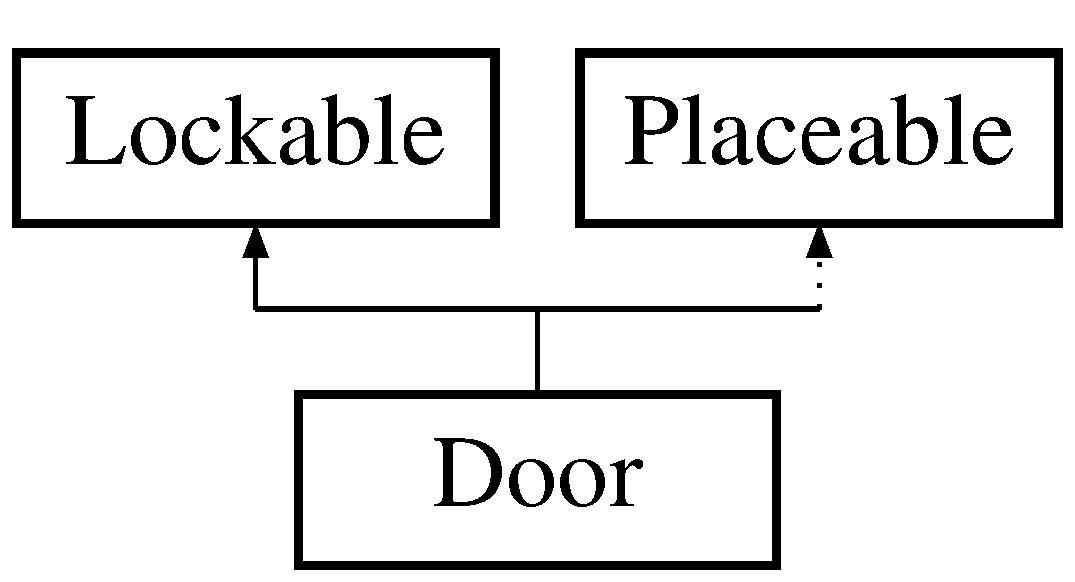
\includegraphics[height=2.000000cm]{class_door}
\end{center}
\end{figure}
\subsection*{Public Member Functions}
\begin{DoxyCompactItemize}
\item 
\hypertarget{class_door_a60ffd182da3a5663b0a1215117b8a3fd}{}\label{class_door_a60ffd182da3a5663b0a1215117b8a3fd} 
void {\bfseries update\+Lvl} (int a\+Level)
\item 
\hypertarget{class_door_a2accb2023adfd41f0b1c2944d48ffd0c}{}\label{class_door_a2accb2023adfd41f0b1c2944d48ffd0c} 
bool {\bfseries open} (\hyperlink{class_key_item}{Key\+Item} $\ast$a\+Key)
\item 
\hypertarget{class_door_a8ec117c3a051d43dba6f571e0068cf48}{}\label{class_door_a8ec117c3a051d43dba6f571e0068cf48} 
const char {\bfseries get\+Symbol} ()
\item 
\hypertarget{class_door_a7736b689448b00c26407c20c8826777f}{}\label{class_door_a7736b689448b00c26407c20c8826777f} 
bool {\bfseries is\+Walkable} ()
\item 
\hypertarget{class_door_a8676c57077d910a740a786ba1885f492}{}\label{class_door_a8676c57077d910a740a786ba1885f492} 
std\+::string {\bfseries key\+Name} ()
\item 
\hypertarget{class_door_a739d0097860e447091024c1dbe57ca55}{}\label{class_door_a739d0097860e447091024c1dbe57ca55} 
bool {\bfseries reset} ()
\end{DoxyCompactItemize}
\subsection*{Friends}
\begin{DoxyCompactItemize}
\item 
\hypertarget{class_door_ac98d07dd8f7b70e16ccb9a01abf56b9c}{}\label{class_door_ac98d07dd8f7b70e16ccb9a01abf56b9c} 
class {\bfseries boost\+::serialization\+::access}
\end{DoxyCompactItemize}
\subsection*{Additional Inherited Members}


\subsection{Detailed Description}


Definition at line 60 of file basic\+\_\+structure.\+h.



The documentation for this class was generated from the following files\+:\begin{DoxyCompactItemize}
\item 
basic\+\_\+structure.\+h\item 
basic\+\_\+structure.\+cpp\end{DoxyCompactItemize}

\hypertarget{class_empty_type_exception}{}\section{Empty\+Type\+Exception Class Reference}
\label{class_empty_type_exception}\index{Empty\+Type\+Exception@{Empty\+Type\+Exception}}
Inheritance diagram for Empty\+Type\+Exception\+:\begin{figure}[H]
\begin{center}
\leavevmode
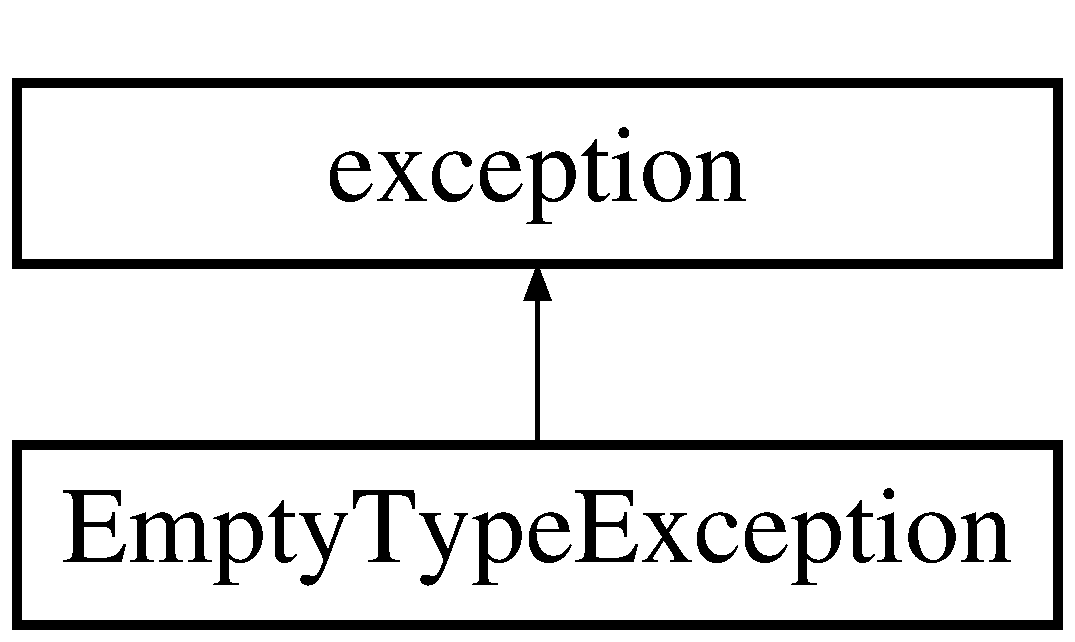
\includegraphics[height=2.000000cm]{class_empty_type_exception}
\end{center}
\end{figure}
\subsection*{Public Member Functions}
\begin{DoxyCompactItemize}
\item 
\hypertarget{class_empty_type_exception_a9396f7f0f9f5cb84f60759a48a3f3590}{}\label{class_empty_type_exception_a9396f7f0f9f5cb84f60759a48a3f3590} 
{\bfseries Empty\+Type\+Exception} (const std\+::string class\+Name)
\item 
\hypertarget{class_empty_type_exception_af5d4c57db2ef804da89c720794fead3f}{}\label{class_empty_type_exception_af5d4c57db2ef804da89c720794fead3f} 
virtual const char $\ast$ {\bfseries what} () const  throw ()
\end{DoxyCompactItemize}


\subsection{Detailed Description}


Definition at line 27 of file inventory\+\_\+exceptions.\+h.



The documentation for this class was generated from the following file\+:\begin{DoxyCompactItemize}
\item 
inventory\+\_\+exceptions.\+h\end{DoxyCompactItemize}

\hypertarget{class_enemy}{}\section{Enemy Class Reference}
\label{class_enemy}\index{Enemy@{Enemy}}
Inheritance diagram for Enemy\+:\begin{figure}[H]
\begin{center}
\leavevmode
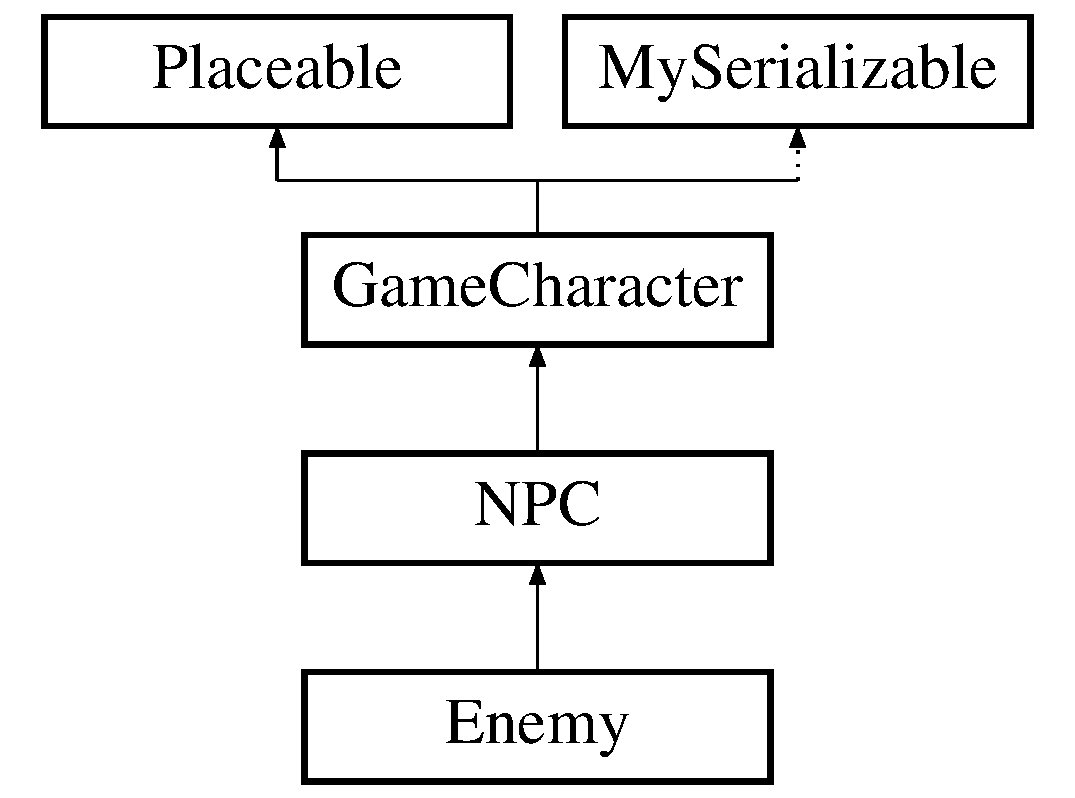
\includegraphics[height=4.000000cm]{class_enemy}
\end{center}
\end{figure}
\subsection*{Public Member Functions}
\begin{DoxyCompactItemize}
\item 
\hypertarget{class_enemy_a64fb6f0fce2338a033588c9115593d21}{}\label{class_enemy_a64fb6f0fce2338a033588c9115593d21} 
{\bfseries Enemy} (std\+::string a\+Name, int a\+Level)
\item 
\hypertarget{class_enemy_ad1b2d1373f3344f23fa438eb73f315d6}{}\label{class_enemy_ad1b2d1373f3344f23fa438eb73f315d6} 
const char {\bfseries get\+Symbol} ()
\item 
\hypertarget{class_enemy_a16d7bdedccabfe8777d2d424a8dbe877}{}\label{class_enemy_a16d7bdedccabfe8777d2d424a8dbe877} 
void {\bfseries get\+Strategy} ()
\item 
\hypertarget{class_enemy_a34898829bc0fd2c0699f4bbe5ac8ed1a}{}\label{class_enemy_a34898829bc0fd2c0699f4bbe5ac8ed1a} 
bool {\bfseries is\+Walkable} ()
\item 
\hypertarget{class_enemy_ae025207363a769591c1accad3d1c2412}{}\label{class_enemy_ae025207363a769591c1accad3d1c2412} 
void {\bfseries load} (std\+::string filename)
\item 
\hypertarget{class_enemy_a186b6812f0fc859f1a67d02bb1a42a16}{}\label{class_enemy_a186b6812f0fc859f1a67d02bb1a42a16} 
void {\bfseries save} (std\+::string filename)
\end{DoxyCompactItemize}
\subsection*{Static Public Member Functions}
\begin{DoxyCompactItemize}
\item 
\hypertarget{class_enemy_a284a2d438cfa8e5de5fb796d351a04bb}{}\label{class_enemy_a284a2d438cfa8e5de5fb796d351a04bb} 
static \hyperlink{class_enemy}{Enemy} {\bfseries s\+Load} (std\+::string filename)
\end{DoxyCompactItemize}
\subsection*{Friends}
\begin{DoxyCompactItemize}
\item 
\hypertarget{class_enemy_ac98d07dd8f7b70e16ccb9a01abf56b9c}{}\label{class_enemy_ac98d07dd8f7b70e16ccb9a01abf56b9c} 
class {\bfseries boost\+::serialization\+::access}
\end{DoxyCompactItemize}


\subsection{Detailed Description}


Definition at line 159 of file character.\+h.



The documentation for this class was generated from the following files\+:\begin{DoxyCompactItemize}
\item 
character.\+h\item 
character.\+cpp\end{DoxyCompactItemize}

\hypertarget{class_equipment}{}\section{Equipment Class Reference}
\label{class_equipment}\index{Equipment@{Equipment}}
Inheritance diagram for Equipment\+:\begin{figure}[H]
\begin{center}
\leavevmode
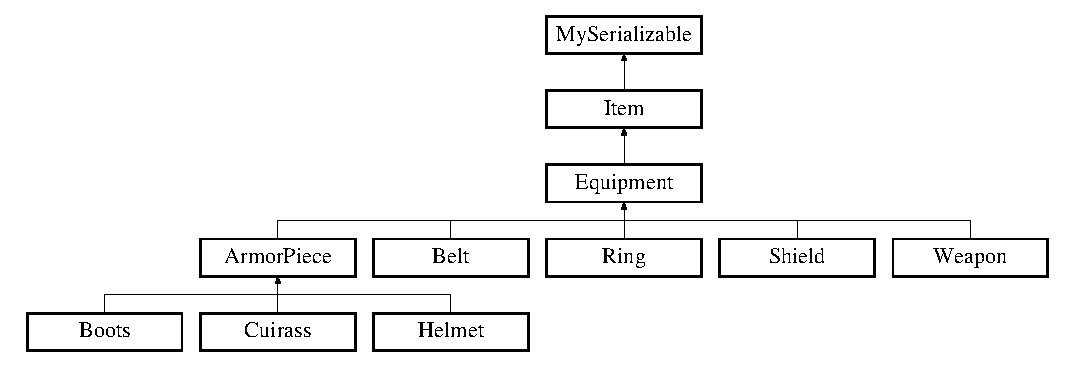
\includegraphics[height=4.487180cm]{class_equipment}
\end{center}
\end{figure}
\subsection*{Public Member Functions}
\begin{DoxyCompactItemize}
\item 
int $\ast$ \hyperlink{class_equipment_a9e2505f187dadc04a811a9d0680d29cf}{get\+All\+Enchantments} ()
\begin{DoxyCompactList}\small\item\em Getter for the Abilities total. \end{DoxyCompactList}\item 
\hypertarget{class_equipment_a562d37bd3587b738c13c262650cf8489}{}\label{class_equipment_a562d37bd3587b738c13c262650cf8489} 
int {\bfseries get\+Enchantment} (\hyperlink{class_ability}{Ability} $\ast$abl)
\item 
\hypertarget{class_equipment_a476657aab86ed7d26a97aa77454f7ac3}{}\label{class_equipment_a476657aab86ed7d26a97aa77454f7ac3} 
int {\bfseries get\+Enchantment} (int index)
\item 
void \hyperlink{class_equipment_ab56d6a16b2151d7793c4b5fddde1f145}{update\+Lvl} (int player\+Level)
\begin{DoxyCompactList}\small\item\em Method to set the enchantment on the item acording to the player level on map load. \end{DoxyCompactList}\item 
\hypertarget{class_equipment_a3d293fd3861ebddc0a4ae1e26d54ff36}{}\label{class_equipment_a3d293fd3861ebddc0a4ae1e26d54ff36} 
virtual int {\bfseries get\+Weight} ()
\item 
\hypertarget{class_equipment_a274e31858324c1774dd022315ee056a9}{}\label{class_equipment_a274e31858324c1774dd022315ee056a9} 
virtual \hyperlink{class_equip_type}{Equip\+Type} const  $\ast$ {\bfseries get\+Type} ()
\item 
\hypertarget{class_equipment_a66ae3c2ca283f3788abbd61b45ee5077}{}\label{class_equipment_a66ae3c2ca283f3788abbd61b45ee5077} 
std\+::string {\bfseries to\+String} ()
\item 
\hypertarget{class_equipment_ac534ea06d524c524201e359f54938146}{}\label{class_equipment_ac534ea06d524c524201e359f54938146} 
virtual void {\bfseries save} (std\+::string filename)
\item 
\hypertarget{class_equipment_ac07ac998f85529e90bd209b32c89809d}{}\label{class_equipment_ac07ac998f85529e90bd209b32c89809d} 
virtual void {\bfseries load} (std\+::string filename)
\end{DoxyCompactItemize}
\subsection*{Protected Member Functions}
\begin{DoxyCompactItemize}
\item 
\hypertarget{class_equipment_ab98d0ccbf2f89274a0c4aa9d4763e35c}{}\label{class_equipment_ab98d0ccbf2f89274a0c4aa9d4763e35c} 
{\bfseries Equipment} (std\+::string a\+Name, \hyperlink{class_equip_type}{Equip\+Type} const $\ast$a\+Type)
\item 
\hypertarget{class_equipment_ac6946f620ba8e13c3dfd039d4c604f09}{}\label{class_equipment_ac6946f620ba8e13c3dfd039d4c604f09} 
virtual void {\bfseries set\+Enchantment} (\hyperlink{class_ability}{Ability} abl, int bonus)
\end{DoxyCompactItemize}
\subsection*{Friends}
\begin{DoxyCompactItemize}
\item 
\hypertarget{class_equipment_ac98d07dd8f7b70e16ccb9a01abf56b9c}{}\label{class_equipment_ac98d07dd8f7b70e16ccb9a01abf56b9c} 
class {\bfseries boost\+::serialization\+::access}
\end{DoxyCompactItemize}


\subsection{Detailed Description}


Definition at line 75 of file inv2.\+h.



\subsection{Member Function Documentation}
\hypertarget{class_equipment_a9e2505f187dadc04a811a9d0680d29cf}{}\label{class_equipment_a9e2505f187dadc04a811a9d0680d29cf} 
\index{Equipment@{Equipment}!get\+All\+Enchantments@{get\+All\+Enchantments}}
\index{get\+All\+Enchantments@{get\+All\+Enchantments}!Equipment@{Equipment}}
\subsubsection{\texorpdfstring{get\+All\+Enchantments()}{getAllEnchantments()}}
{\footnotesize\ttfamily int $\ast$ Equipment\+::get\+All\+Enchantments (\begin{DoxyParamCaption}{ }\end{DoxyParamCaption})}



Getter for the Abilities total. 

\begin{DoxyReturn}{Returns}
will returns the Abilities result 
\end{DoxyReturn}


Definition at line 58 of file inv2.\+cpp.


\begin{DoxyCode}
59 \{
60     \textcolor{keywordtype}{int}* result = \textcolor{keyword}{new} \textcolor{keywordtype}{int}[Ability::getCount()];
61     \textcolor{keywordtype}{int} i;
62 
63     \textcolor{keywordflow}{for} (i = 0; i < Ability::getCount(); i++)
64     \{
65         \textcolor{keywordflow}{if} (this->getType()->isAllowed(i))
66         \{
67             result[i] = enchantments[i];
68         \}
69         \textcolor{keywordflow}{else}
70         \{
71             result[i] = 0;
72         \}
73     \}
74 
75     \textcolor{keywordflow}{return} result;
76 \}
\end{DoxyCode}
\hypertarget{class_equipment_ab56d6a16b2151d7793c4b5fddde1f145}{}\label{class_equipment_ab56d6a16b2151d7793c4b5fddde1f145} 
\index{Equipment@{Equipment}!update\+Lvl@{update\+Lvl}}
\index{update\+Lvl@{update\+Lvl}!Equipment@{Equipment}}
\subsubsection{\texorpdfstring{update\+Lvl()}{updateLvl()}}
{\footnotesize\ttfamily void Equipment\+::update\+Lvl (\begin{DoxyParamCaption}\item[{int}]{player\+Level }\end{DoxyParamCaption})\hspace{0.3cm}{\ttfamily [virtual]}}



Method to set the enchantment on the item acording to the player level on map load. 


\begin{DoxyParams}{Parameters}
{\em player\+Level} & give the player level to set the Abilities (the ones that are on enchantments (1)) to it\textquotesingle{}s level \\
\hline
\end{DoxyParams}


Reimplemented from \hyperlink{class_item}{Item}.



Definition at line 135 of file inv2.\+cpp.


\begin{DoxyCode}
136 \{
137     vector<Ability> allowed = this->getType()->getEnchantments();
138     \textcolor{keywordtype}{int} points = playerLevel;
139     \textcolor{keywordtype}{int} bonus;
140     \textcolor{keywordtype}{float} rnd;
141 
142     \textcolor{keywordflow}{for} (\hyperlink{class_ability}{Ability} a : allowed)
143     \{
144         rnd = ( rand() % 100) / 100.0;
145         bonus = min(points, min((\textcolor{keywordtype}{int})(rnd * points), 5));
146         \textcolor{comment}{//cout << "rnd:" << rnd << "  points:" << points << "  bonus:" << bonus << endl;}
147         enchantments[a.index] = bonus;
148         points -= bonus;
149     \}
150 \}
\end{DoxyCode}


The documentation for this class was generated from the following files\+:\begin{DoxyCompactItemize}
\item 
inv2.\+h\item 
inv2.\+cpp\end{DoxyCompactItemize}

\hypertarget{class_equip_type}{}\section{Equip\+Type Class Reference}
\label{class_equip_type}\index{Equip\+Type@{Equip\+Type}}
\subsection*{Public Member Functions}
\begin{DoxyCompactItemize}
\item 
\hypertarget{class_equip_type_a05327988569e884c73fe56aecfb5c31e}{}\label{class_equip_type_a05327988569e884c73fe56aecfb5c31e} 
vector$<$ \hyperlink{class_ability}{Ability} $>$ {\bfseries get\+Enchantments} () const
\item 
\hypertarget{class_equip_type_adc5b044a73400362f38078e25b242272}{}\label{class_equip_type_adc5b044a73400362f38078e25b242272} 
const bool {\bfseries is\+Allowed} (const \hyperlink{class_ability}{Ability} abl) const
\item 
\hypertarget{class_equip_type_a1cf5a5d3ab3ff6bd9da46061073e23ec}{}\label{class_equip_type_a1cf5a5d3ab3ff6bd9da46061073e23ec} 
const bool {\bfseries is\+Allowed} (int an\+Index) const
\end{DoxyCompactItemize}
\subsection*{Static Public Member Functions}
\begin{DoxyCompactItemize}
\item 
\hypertarget{class_equip_type_abb382741bb477afd8ee58971dbbde300}{}\label{class_equip_type_abb382741bb477afd8ee58971dbbde300} 
static const int {\bfseries get\+Count} ()
\end{DoxyCompactItemize}
\subsection*{Public Attributes}
\begin{DoxyCompactItemize}
\item 
\hypertarget{class_equip_type_a62ce6b1e8a21549560eb00ae4cf70e3d}{}\label{class_equip_type_a62ce6b1e8a21549560eb00ae4cf70e3d} 
const std\+::unordered\+\_\+set$<$ const \hyperlink{class_ability}{Ability} $\ast$ $>$ {\bfseries stats}
\item 
\hypertarget{class_equip_type_a7f5c248cfd8972043915fab139c49309}{}\label{class_equip_type_a7f5c248cfd8972043915fab139c49309} 
const int {\bfseries index}
\item 
\hypertarget{class_equip_type_a1b05978633df80f88bf0a6b1497308d4}{}\label{class_equip_type_a1b05978633df80f88bf0a6b1497308d4} 
const std\+::string {\bfseries name}
\end{DoxyCompactItemize}
\subsection*{Static Public Attributes}
\begin{DoxyCompactItemize}
\item 
\hypertarget{class_equip_type_a0ad3a2f66447465ec7bcf023517aad4d}{}\label{class_equip_type_a0ad3a2f66447465ec7bcf023517aad4d} 
static const \hyperlink{class_equip_type}{Equip\+Type} {\bfseries H\+E\+L\+M\+ET} = \hyperlink{class_equip_type}{Equip\+Type}(\char`\"{}Helmet\char`\"{}, std\+::unordered\+\_\+set$<$const \hyperlink{class_ability}{Ability}$\ast$$>$\{ \&Ability\+::\+I\+N\+TL, \&Ability\+::\+W\+IS, \&Ability\+::\+AC \})
\item 
\hypertarget{class_equip_type_a75eb1f613017700885b5ba17b869288f}{}\label{class_equip_type_a75eb1f613017700885b5ba17b869288f} 
static const \hyperlink{class_equip_type}{Equip\+Type} {\bfseries C\+U\+I\+R\+A\+SS} = \hyperlink{class_equip_type}{Equip\+Type}(\char`\"{}Armor\char`\"{}, std\+::unordered\+\_\+set$<$const \hyperlink{class_ability}{Ability}$\ast$$>$\{ \&Ability\+::\+AC \})
\item 
\hypertarget{class_equip_type_ad4fcb251950aa992744f8fa8501a830f}{}\label{class_equip_type_ad4fcb251950aa992744f8fa8501a830f} 
static const \hyperlink{class_equip_type}{Equip\+Type} {\bfseries B\+O\+O\+TS} = \hyperlink{class_equip_type}{Equip\+Type}(\char`\"{}Boots\char`\"{}, std\+::unordered\+\_\+set$<$const \hyperlink{class_ability}{Ability}$\ast$$>$\{ \&Ability\+::\+AC, \&Ability\+::\+S\+TR, \&Ability\+::\+C\+ON, \&Ability\+::\+W\+IS, \&Ability\+::\+C\+HA \})
\item 
\hypertarget{class_equip_type_ac6d91237e6bf68bceda1b19e57022b42}{}\label{class_equip_type_ac6d91237e6bf68bceda1b19e57022b42} 
static const \hyperlink{class_equip_type}{Equip\+Type} {\bfseries R\+I\+NG} = \hyperlink{class_equip_type}{Equip\+Type}(\char`\"{}Ring\char`\"{}, std\+::unordered\+\_\+set$<$const \hyperlink{class_ability}{Ability}$\ast$$>$\{ \&Ability\+::\+S\+TR, \&Ability\+::\+C\+ON \})
\item 
\hypertarget{class_equip_type_a09cc664449dd4ade565f79e45c835f95}{}\label{class_equip_type_a09cc664449dd4ade565f79e45c835f95} 
static const \hyperlink{class_equip_type}{Equip\+Type} {\bfseries B\+E\+LT} = \hyperlink{class_equip_type}{Equip\+Type}(\char`\"{}Belt\char`\"{}, std\+::unordered\+\_\+set$<$const \hyperlink{class_ability}{Ability}$\ast$$>$\{ \&Ability\+::\+AC, \&Ability\+::\+D\+EX \})
\item 
\hypertarget{class_equip_type_a49babc5bcad67546676717becb5a4c40}{}\label{class_equip_type_a49babc5bcad67546676717becb5a4c40} 
static const \hyperlink{class_equip_type}{Equip\+Type} {\bfseries S\+H\+I\+E\+LD} = \hyperlink{class_equip_type}{Equip\+Type}(\char`\"{}Shield\char`\"{}, std\+::unordered\+\_\+set$<$const \hyperlink{class_ability}{Ability}$\ast$$>$\{ \&Ability\+::\+AC \})
\item 
\hypertarget{class_equip_type_a7897c25db67405c77cb0237c0c49c7c5}{}\label{class_equip_type_a7897c25db67405c77cb0237c0c49c7c5} 
static const \hyperlink{class_equip_type}{Equip\+Type} {\bfseries W\+E\+A\+P\+ON} = \hyperlink{class_equip_type}{Equip\+Type}(\char`\"{}Weapon\char`\"{}, std\+::unordered\+\_\+set$<$const \hyperlink{class_ability}{Ability}$\ast$$>$\{ \&Ability\+::\+A\+TK, \&Ability\+::\+D\+MG \})
\end{DoxyCompactItemize}


\subsection{Detailed Description}


Definition at line 82 of file config.\+h.



The documentation for this class was generated from the following files\+:\begin{DoxyCompactItemize}
\item 
config.\+h\item 
config.\+cpp\end{DoxyCompactItemize}

\hypertarget{class_friendly}{}\section{Friendly Class Reference}
\label{class_friendly}\index{Friendly@{Friendly}}
Inheritance diagram for Friendly\+:\begin{figure}[H]
\begin{center}
\leavevmode
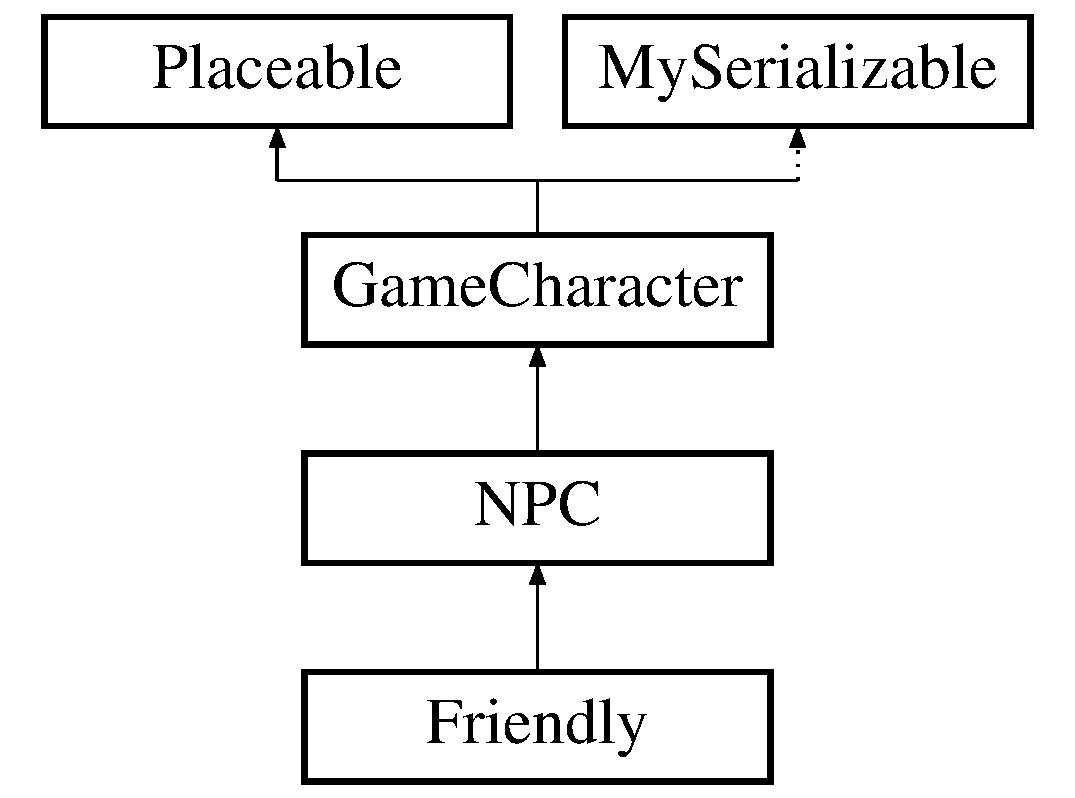
\includegraphics[height=4.000000cm]{class_friendly}
\end{center}
\end{figure}
\subsection*{Public Member Functions}
\begin{DoxyCompactItemize}
\item 
\hypertarget{class_friendly_a659e9fb5059bd5aecccfde31268cfeae}{}\label{class_friendly_a659e9fb5059bd5aecccfde31268cfeae} 
{\bfseries Friendly} (std\+::string a\+Name, int a\+Base\+Atk, int a\+Level)
\item 
\hypertarget{class_friendly_a545e6be79496bbcf92bddf6d969119a1}{}\label{class_friendly_a545e6be79496bbcf92bddf6d969119a1} 
const std\+::string {\bfseries get\+Symbol} ()
\item 
\hypertarget{class_friendly_aa309d676f0034511f83386108798c1e2}{}\label{class_friendly_aa309d676f0034511f83386108798c1e2} 
bool {\bfseries is\+Walkable} ()
\item 
\hypertarget{class_friendly_a4fe8e4947182ee452ecb67b1a5da81e8}{}\label{class_friendly_a4fe8e4947182ee452ecb67b1a5da81e8} 
void {\bfseries get\+Strategy} ()
\item 
\hypertarget{class_friendly_a1445b856d8c440c3bee4dc1ae63c0b4f}{}\label{class_friendly_a1445b856d8c440c3bee4dc1ae63c0b4f} 
void {\bfseries load} (std\+::string filename)
\item 
\hypertarget{class_friendly_ab757441afa46a0928dc52da262318699}{}\label{class_friendly_ab757441afa46a0928dc52da262318699} 
void {\bfseries save} (std\+::string filename)
\end{DoxyCompactItemize}
\subsection*{Static Public Member Functions}
\begin{DoxyCompactItemize}
\item 
\hypertarget{class_friendly_aed039045cd15d26708634105abbea232}{}\label{class_friendly_aed039045cd15d26708634105abbea232} 
static \hyperlink{class_friendly}{Friendly} {\bfseries s\+Load} (std\+::string filename)
\end{DoxyCompactItemize}
\subsection*{Friends}
\begin{DoxyCompactItemize}
\item 
\hypertarget{class_friendly_ac98d07dd8f7b70e16ccb9a01abf56b9c}{}\label{class_friendly_ac98d07dd8f7b70e16ccb9a01abf56b9c} 
class {\bfseries boost\+::serialization\+::access}
\end{DoxyCompactItemize}


\subsection{Detailed Description}


Definition at line 212 of file character.\+h.



The documentation for this class was generated from the following files\+:\begin{DoxyCompactItemize}
\item 
character.\+h\item 
character.\+cpp\end{DoxyCompactItemize}

\hypertarget{class_game}{}\section{Game Class Reference}
\label{class_game}\index{Game@{Game}}
\subsection*{Public Member Functions}
\begin{DoxyCompactItemize}
\item 
\hypertarget{class_game_a0592b20bb4dafc38a3cfdb7c5f5e963f}{}\label{class_game_a0592b20bb4dafc38a3cfdb7c5f5e963f} 
{\bfseries Game} (\hyperlink{class_map}{Map} $\ast$a\+Map, \hyperlink{class_player}{Player} $\ast$a\+Player)
\item 
\hypertarget{class_game_a18d94ea20a9e7085faf15b0abb83a87c}{}\label{class_game_a18d94ea20a9e7085faf15b0abb83a87c} 
\hyperlink{class_game}{Game} {\bfseries get\+Instance} ()
\item 
\hypertarget{class_game_a801658c7cef474bc1d9a830f4a79034c}{}\label{class_game_a801658c7cef474bc1d9a830f4a79034c} 
void {\bfseries next\+Turn} ()
\item 
\hypertarget{class_game_a5d22cebed1061d51b2c3aaba2352972d}{}\label{class_game_a5d22cebed1061d51b2c3aaba2352972d} 
\hyperlink{class_player}{Player} {\bfseries load\+Player} ()
\item 
\hypertarget{class_game_ac7c8b111e2f09bbcf92a3da037992e57}{}\label{class_game_ac7c8b111e2f09bbcf92a3da037992e57} 
\hyperlink{class_map}{Map} {\bfseries load\+Map} ()
\item 
\hypertarget{class_game_ae8638ccdb0ef3bf39a6affa30aa1258f}{}\label{class_game_ae8638ccdb0ef3bf39a6affa30aa1258f} 
void {\bfseries start\+Game} ()
\item 
\hypertarget{class_game_a9e5b2d2156debcd958e2eae6fc79730a}{}\label{class_game_a9e5b2d2156debcd958e2eae6fc79730a} 
void {\bfseries create\+Player} ()
\item 
\hypertarget{class_game_a94515881419e23477226deba95dbb1f3}{}\label{class_game_a94515881419e23477226deba95dbb1f3} 
void {\bfseries create\+Player\+From\+Load} ()
\item 
\hypertarget{class_game_ac3276ead57322cccdeed919fd7f28b34}{}\label{class_game_ac3276ead57322cccdeed919fd7f28b34} 
void {\bfseries map\+Editor} (\hyperlink{class_map}{Map} map)
\item 
void \hyperlink{class_game_ac8c66f86b907bc8afc33c8e31b800611}{display} (\hyperlink{class_game_character}{Game\+Character} $\ast$gh)
\end{DoxyCompactItemize}


\subsection{Detailed Description}


Definition at line 13 of file game.\+h.



\subsection{Member Function Documentation}
\hypertarget{class_game_ac8c66f86b907bc8afc33c8e31b800611}{}\label{class_game_ac8c66f86b907bc8afc33c8e31b800611} 
\index{Game@{Game}!display@{display}}
\index{display@{display}!Game@{Game}}
\subsubsection{\texorpdfstring{display()}{display()}}
{\footnotesize\ttfamily void Game\+::display (\begin{DoxyParamCaption}\item[{\hyperlink{class_game_character}{Game\+Character} $\ast$}]{gh }\end{DoxyParamCaption})}

Display the inventory, worn items and backpack 
\begin{DoxyParams}{Parameters}
{\em } & Call to string methods \\
\hline
\end{DoxyParams}


Definition at line 654 of file game.\+cpp.


\begin{DoxyCode}
654                                    \{
655 
656     \textcolor{comment}{//Before the information, the display of attacks and rounds are here..}
657     \textcolor{comment}{//example...}
658 
659     cout << \textcolor{stringliteral}{"\(\backslash\)n\_\_\_\_\_\_\_\_\_\_\_\_\_\_\_\_\_\_\_\_\_\_\_\_\_\_\_\_\_\_\_\_INFORMATIONS\_\_\_\_\_\_\_\_\_\_\_\_\_\_\_\_\_\_\_\_\_\_\_\_\_\_\_\_\_\_\_\_\_\_\_\_\_\_\_\_\_\(\backslash\)n"};
660     \textcolor{comment}{//Call the character in play to display what he has.}
661     \textcolor{comment}{//This calls ---> }
662     cout << gh->toString();
663 
664     \textcolor{comment}{//equip/unequip...to be added here!!!! }
665     cout << \textcolor{stringliteral}{"\(\backslash\)n\(\backslash\)nEQUIP/UNEQUIP\_\_\_\_PRESS P"}<<endl;
666     cout << \textcolor{stringliteral}{"BACK\_\_\_\_\_\_\_\_\_\_\_\_\_PRESS B"} << endl;
667     
668 \}
\end{DoxyCode}


The documentation for this class was generated from the following files\+:\begin{DoxyCompactItemize}
\item 
game.\+h\item 
game.\+cpp\end{DoxyCompactItemize}

\hypertarget{class_game_character}{}\section{Game\+Character Class Reference}
\label{class_game_character}\index{Game\+Character@{Game\+Character}}


Base class for character types \hyperlink{class_player}{Player}, Npc\+Enepmy and \hyperlink{class_friendly}{Friendly}.  




{\ttfamily \#include $<$character.\+h$>$}

Inheritance diagram for Game\+Character\+:\begin{figure}[H]
\begin{center}
\leavevmode
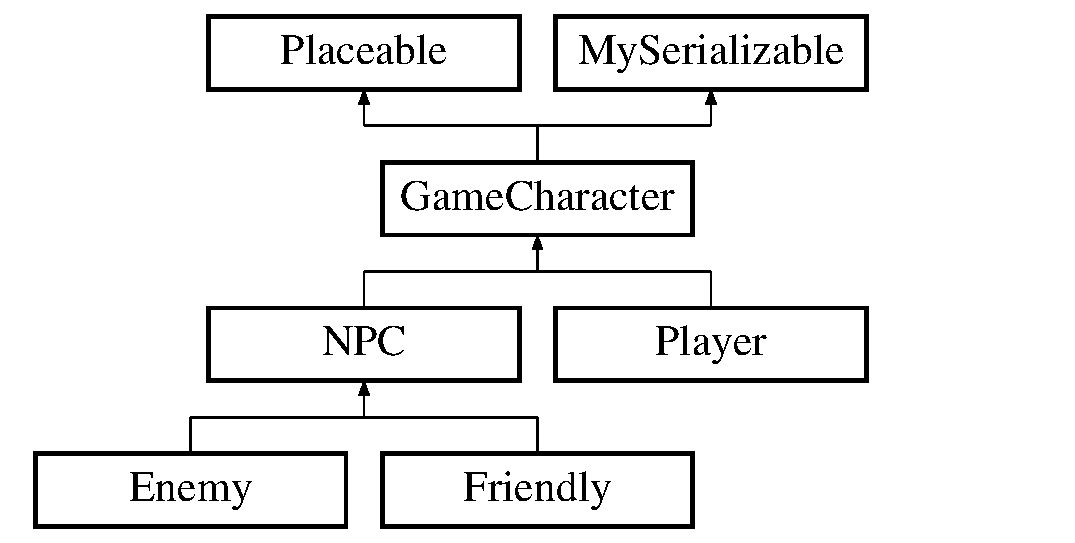
\includegraphics[height=4.000000cm]{class_game_character}
\end{center}
\end{figure}
\subsection*{Public Member Functions}
\begin{DoxyCompactItemize}
\item 
\hypertarget{class_game_character_ad5aee02539362a4d081bb87dd0192995}{}\label{class_game_character_ad5aee02539362a4d081bb87dd0192995} 
{\bfseries Game\+Character} (std\+::string a\+Name, int a\+Level)
\item 
\hypertarget{class_game_character_a175c4c67c7276a9c64833afbccf392ee}{}\label{class_game_character_a175c4c67c7276a9c64833afbccf392ee} 
const char {\bfseries get\+Symbol} ()
\item 
\hypertarget{class_game_character_a1acb3766c648348716a1b162626d6ffa}{}\label{class_game_character_a1acb3766c648348716a1b162626d6ffa} 
std\+::string {\bfseries get\+Name} ()
\item 
\hypertarget{class_game_character_af11d88fb41e0ec3f7711e18e63be62f4}{}\label{class_game_character_af11d88fb41e0ec3f7711e18e63be62f4} 
void {\bfseries set\+Name} (std\+::string a\+Name)
\item 
\hypertarget{class_game_character_ad36b2f145cd55553ded91242a9c929ce}{}\label{class_game_character_ad36b2f145cd55553ded91242a9c929ce} 
virtual bool {\bfseries reset} ()
\item 
\hypertarget{class_game_character_aa989c9d337840ce0f103dc102351b282}{}\label{class_game_character_aa989c9d337840ce0f103dc102351b282} 
void {\bfseries reset\+Level} ()
\item 
\hypertarget{class_game_character_a092512872c1d5e2d41484a6cf82cab81}{}\label{class_game_character_a092512872c1d5e2d41484a6cf82cab81} 
bool {\bfseries unlock} ()
\item 
\hypertarget{class_game_character_a31aa568d3cb993da2592926d49ab5457}{}\label{class_game_character_a31aa568d3cb993da2592926d49ab5457} 
int {\bfseries get\+Level} ()
\item 
void \hyperlink{class_game_character_a367a537148a995677d9649b975cb326b}{level\+Up} ()
\begin{DoxyCompactList}\small\item\em Function for a single level increment. \end{DoxyCompactList}\item 
virtual void \hyperlink{class_game_character_a0e6839e7c79e97ba7daea9ed0fc2569e}{update\+Lvl} (int a\+Level)
\begin{DoxyCompactList}\small\item\em Function to set a characters level. \end{DoxyCompactList}\item 
\hypertarget{class_game_character_a65326d8f34ef36911b58b1654dce357b}{}\label{class_game_character_a65326d8f34ef36911b58b1654dce357b} 
\hyperlink{class_inventory}{Inventory} {\bfseries get\+Inventory} ()
\item 
int $\ast$ \hyperlink{class_game_character_a9b1de762235904d9f11147780ffb45f1}{get\+All\+Base\+Abl} ()
\item 
\hypertarget{class_game_character_ac7dd71d84cef1fa1cc31787c2a2f02aa}{}\label{class_game_character_ac7dd71d84cef1fa1cc31787c2a2f02aa} 
int \hyperlink{class_game_character_ac7dd71d84cef1fa1cc31787c2a2f02aa}{get\+Base\+Abl} (\hyperlink{class_ability}{Ability} abl)
\begin{DoxyCompactList}\small\item\em Function that returns a single base ability of a character. \end{DoxyCompactList}\item 
\hypertarget{class_game_character_af604f6f1df72988de0b3f34625844545}{}\label{class_game_character_af604f6f1df72988de0b3f34625844545} 
void \hyperlink{class_game_character_af604f6f1df72988de0b3f34625844545}{set\+Base\+Abl} (\hyperlink{class_ability}{Ability} abl, int value)
\begin{DoxyCompactList}\small\item\em Function that sets a single requested base ability of a character. \end{DoxyCompactList}\item 
int $\ast$ \hyperlink{class_game_character_a369f58b909a9ac72e572cd5c65773779}{get\+All\+Bonus} ()
\item 
\hypertarget{class_game_character_ab7f1c82a0451f417dad7651c55d96880}{}\label{class_game_character_ab7f1c82a0451f417dad7651c55d96880} 
int \hyperlink{class_game_character_ab7f1c82a0451f417dad7651c55d96880}{get\+Bonus} (\hyperlink{class_ability}{Ability} abl)
\begin{DoxyCompactList}\small\item\em Function that returns a single ability bonus of a character. \end{DoxyCompactList}\item 
int $\ast$ \hyperlink{class_game_character_ab70746cb0cd382cbe56c0190a03a3024}{get\+All\+Net\+Stats} ()
\item 
int \hyperlink{class_game_character_a94e6371f4f2f14c6a9e6aa9c8e78775b}{get\+Net\+Stat} (\hyperlink{class_ability}{Ability} abl)
\item 
\hypertarget{class_game_character_abbe3c5c7e6de419f6e14aaa74b91c60d}{}\label{class_game_character_abbe3c5c7e6de419f6e14aaa74b91c60d} 
bool {\bfseries add\+To\+Pack} (\hyperlink{class_item}{Item} $\ast$an\+Item)
\item 
\hypertarget{class_game_character_af8e3c23dd71472b27f3daa860e88beef}{}\label{class_game_character_af8e3c23dd71472b27f3daa860e88beef} 
void {\bfseries remove\+From\+Pack} (\hyperlink{class_item}{Item} $\ast$an\+Item)
\item 
\hypertarget{class_game_character_a8774e9795a985ae6ba05a6f29cd18074}{}\label{class_game_character_a8774e9795a985ae6ba05a6f29cd18074} 
bool {\bfseries equip} (\hyperlink{class_equipment}{Equipment} $\ast$an\+Item)
\item 
\hypertarget{class_game_character_a6a281827355113352486a9a71882b110}{}\label{class_game_character_a6a281827355113352486a9a71882b110} 
bool {\bfseries unequip} (\hyperlink{class_equip_type}{Equip\+Type} a\+Type)
\item 
\hypertarget{class_game_character_af8c976c875abf76993e716533a25a7b6}{}\label{class_game_character_af8c976c875abf76993e716533a25a7b6} 
std\+::string {\bfseries to\+String} ()
\item 
\hypertarget{class_game_character_ad3656092f8da6899751616597295418b}{}\label{class_game_character_ad3656092f8da6899751616597295418b} 
virtual void {\bfseries load} (std\+::string filename)
\item 
\hypertarget{class_game_character_a37ea5f779910d981baec0ae871a1c097}{}\label{class_game_character_a37ea5f779910d981baec0ae871a1c097} 
virtual void {\bfseries save} (std\+::string filename)
\end{DoxyCompactItemize}
\subsection*{Friends}
\begin{DoxyCompactItemize}
\item 
\hypertarget{class_game_character_ac98d07dd8f7b70e16ccb9a01abf56b9c}{}\label{class_game_character_ac98d07dd8f7b70e16ccb9a01abf56b9c} 
class {\bfseries boost\+::serialization\+::access}
\end{DoxyCompactItemize}


\subsection{Detailed Description}
Base class for character types \hyperlink{class_player}{Player}, Npc\+Enepmy and \hyperlink{class_friendly}{Friendly}. 

The \hyperlink{class_game_character}{Game\+Character} object holds the the name, level, ability scores, bonus, modifiers, and \hyperlink{class_inventory}{Inventory} of a character. It derives extends the abstract class \hyperlink{class_placeable}{Placeable}. 

Definition at line 20 of file character.\+h.



\subsection{Member Function Documentation}
\hypertarget{class_game_character_a9b1de762235904d9f11147780ffb45f1}{}\label{class_game_character_a9b1de762235904d9f11147780ffb45f1} 
\index{Game\+Character@{Game\+Character}!get\+All\+Base\+Abl@{get\+All\+Base\+Abl}}
\index{get\+All\+Base\+Abl@{get\+All\+Base\+Abl}!Game\+Character@{Game\+Character}}
\subsubsection{\texorpdfstring{get\+All\+Base\+Abl()}{getAllBaseAbl()}}
{\footnotesize\ttfamily int $\ast$ Game\+Character\+::get\+All\+Base\+Abl (\begin{DoxyParamCaption}{ }\end{DoxyParamCaption})}

Function that returns an array of a character base ability scores 

Definition at line 127 of file character.\+cpp.


\begin{DoxyCode}
128 \{
129     \textcolor{keywordtype}{int}* result = \textcolor{keyword}{new} \textcolor{keywordtype}{int}[Ability::getCount()];
130     \textcolor{keywordtype}{int} i;
131 
132     \textcolor{keywordflow}{for} (i = 0; i < Ability::getCount(); i++)
133     \{
134         result[i] = abilities[i];
135     \}
136 
137     \textcolor{keywordflow}{return} result;
138 \}
\end{DoxyCode}
\hypertarget{class_game_character_a369f58b909a9ac72e572cd5c65773779}{}\label{class_game_character_a369f58b909a9ac72e572cd5c65773779} 
\index{Game\+Character@{Game\+Character}!get\+All\+Bonus@{get\+All\+Bonus}}
\index{get\+All\+Bonus@{get\+All\+Bonus}!Game\+Character@{Game\+Character}}
\subsubsection{\texorpdfstring{get\+All\+Bonus()}{getAllBonus()}}
{\footnotesize\ttfamily int $\ast$ Game\+Character\+::get\+All\+Bonus (\begin{DoxyParamCaption}{ }\end{DoxyParamCaption})}

Function that returns an array of a character ability bonus. 

Definition at line 154 of file character.\+cpp.


\begin{DoxyCode}
155 \{
156     \textcolor{keywordtype}{int}* result = \textcolor{keyword}{new} \textcolor{keywordtype}{int}[Ability::getCount()];
157     \textcolor{keywordtype}{int} i;
158 
159     \textcolor{keywordflow}{for} (i = 0; i < Ability::getCount(); i++)
160     \{
161         result[i] = bonus[i];
162     \}
163 
164     \textcolor{keywordflow}{return} result;
165 \}
\end{DoxyCode}
\hypertarget{class_game_character_ab70746cb0cd382cbe56c0190a03a3024}{}\label{class_game_character_ab70746cb0cd382cbe56c0190a03a3024} 
\index{Game\+Character@{Game\+Character}!get\+All\+Net\+Stats@{get\+All\+Net\+Stats}}
\index{get\+All\+Net\+Stats@{get\+All\+Net\+Stats}!Game\+Character@{Game\+Character}}
\subsubsection{\texorpdfstring{get\+All\+Net\+Stats()}{getAllNetStats()}}
{\footnotesize\ttfamily int $\ast$ Game\+Character\+::get\+All\+Net\+Stats (\begin{DoxyParamCaption}{ }\end{DoxyParamCaption})}

Function that returns an array of a character net ability scores, with bonus and modifiers included 

Definition at line 204 of file character.\+cpp.


\begin{DoxyCode}
205 \{
206     \textcolor{keywordtype}{int}* result = \textcolor{keyword}{new} \textcolor{keywordtype}{int}[Ability::getCount()];
207     \textcolor{keywordtype}{int}* enchantments = inventory.getAllEquipMods();
208     \textcolor{keywordtype}{int} i;
209 
210     \textcolor{keywordflow}{for} (i = 0; i < Ability::getCount(); i++)
211     \{
212         result[i] = abilities[i] + enchantments[i];
213         \textcolor{comment}{//result[i] = abilities[i] + modifiers[i] + itemModifiers[i];}
214     \}
215 
216     \textcolor{keywordflow}{return} result;
217 \}
\end{DoxyCode}
\hypertarget{class_game_character_a94e6371f4f2f14c6a9e6aa9c8e78775b}{}\label{class_game_character_a94e6371f4f2f14c6a9e6aa9c8e78775b} 
\index{Game\+Character@{Game\+Character}!get\+Net\+Stat@{get\+Net\+Stat}}
\index{get\+Net\+Stat@{get\+Net\+Stat}!Game\+Character@{Game\+Character}}
\subsubsection{\texorpdfstring{get\+Net\+Stat()}{getNetStat()}}
{\footnotesize\ttfamily int Game\+Character\+::get\+Net\+Stat (\begin{DoxyParamCaption}\item[{\hyperlink{class_ability}{Ability}}]{abl }\end{DoxyParamCaption})}

Function that returns a single net ability score of a character, with bonus and modifiers included. 

Definition at line 221 of file character.\+cpp.


\begin{DoxyCode}
222 \{
223     \textcolor{keywordflow}{return} abilities[abl.index]
224         + bonus[abl.index]
225         \textcolor{comment}{//+ modifiers[abl.index]}
226         + inventory.getEquipMod(abl);
227 \}
\end{DoxyCode}
\hypertarget{class_game_character_a367a537148a995677d9649b975cb326b}{}\label{class_game_character_a367a537148a995677d9649b975cb326b} 
\index{Game\+Character@{Game\+Character}!level\+Up@{level\+Up}}
\index{level\+Up@{level\+Up}!Game\+Character@{Game\+Character}}
\subsubsection{\texorpdfstring{level\+Up()}{levelUp()}}
{\footnotesize\ttfamily void Game\+Character\+::level\+Up (\begin{DoxyParamCaption}{ }\end{DoxyParamCaption})}



Function for a single level increment. 

The function gives the character an ability point every 4 levels, as per D\&D rules (here randomly) 

Definition at line 80 of file character.\+cpp.


\begin{DoxyCode}
81 \{
82     \textcolor{keywordtype}{int} i;
83 
84     level++;
85 
86     \textcolor{comment}{//randomly increase an ability bonus each 4 levels.}
87     \textcolor{keywordflow}{if} (level % 4 == 0)
88     \{
89         i = rand() % 6;
90         bonus[Ability::getMainAbls()[i].index]++;
91     \}
92 
93     updateBonus();
94 
95     abilities[Ability::HP.index] += this->hitDie();
96     Hp = abilities[Ability::HP.index];
97 \}
\end{DoxyCode}
\hypertarget{class_game_character_a0e6839e7c79e97ba7daea9ed0fc2569e}{}\label{class_game_character_a0e6839e7c79e97ba7daea9ed0fc2569e} 
\index{Game\+Character@{Game\+Character}!update\+Lvl@{update\+Lvl}}
\index{update\+Lvl@{update\+Lvl}!Game\+Character@{Game\+Character}}
\subsubsection{\texorpdfstring{update\+Lvl()}{updateLvl()}}
{\footnotesize\ttfamily void Game\+Character\+::update\+Lvl (\begin{DoxyParamCaption}\item[{int}]{to\+Level }\end{DoxyParamCaption})\hspace{0.3cm}{\ttfamily [virtual]}}



Function to set a characters level. 

The function calls on Game\+Character\+::level\+UP to ensure the character stats move up accordingly 

Implements \hyperlink{class_placeable}{Placeable}.



Definition at line 102 of file character.\+cpp.


\begin{DoxyCode}
103 \{
104     \textcolor{keywordflow}{if} (toLevel < 0) toLevel = 0;
105 
106     \textcolor{keywordflow}{if} (level == 0 && toLevel > 0) inventory.updateLvl(toLevel);
107     
108     \textcolor{keywordflow}{while} (level < toLevel) this->\hyperlink{class_game_character_a367a537148a995677d9649b975cb326b}{levelUp}();
109 \}
\end{DoxyCode}


The documentation for this class was generated from the following files\+:\begin{DoxyCompactItemize}
\item 
character.\+h\item 
character.\+cpp\end{DoxyCompactItemize}

\hypertarget{class_helmet}{}\section{Helmet Class Reference}
\label{class_helmet}\index{Helmet@{Helmet}}


{\ttfamily \#include $<$inv2.\+h$>$}

Inheritance diagram for Helmet\+:\begin{figure}[H]
\begin{center}
\leavevmode
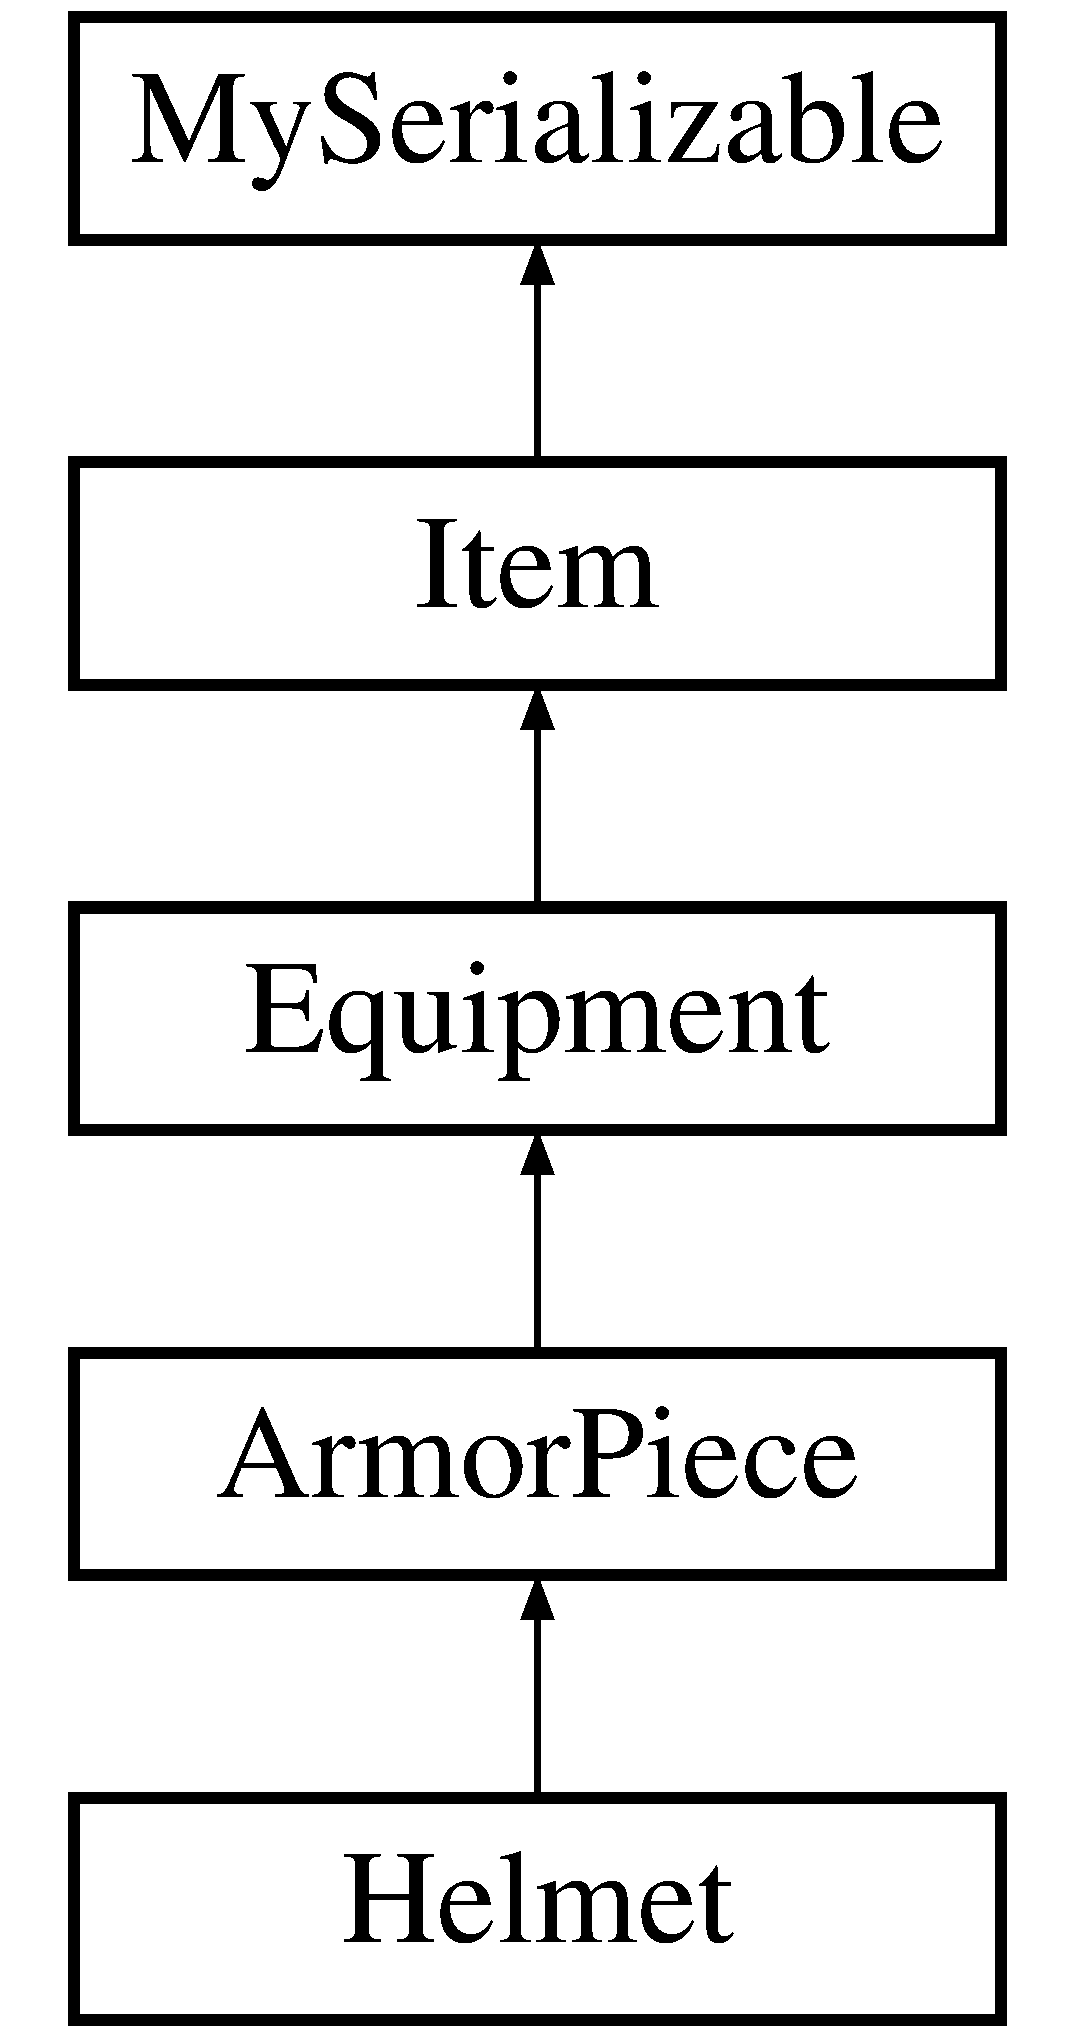
\includegraphics[height=5.000000cm]{class_helmet}
\end{center}
\end{figure}
\subsection*{Public Member Functions}
\begin{DoxyCompactItemize}
\item 
\hypertarget{class_helmet_a41c9d814d15f0f049412a61daef14c41}{}\label{class_helmet_a41c9d814d15f0f049412a61daef14c41} 
{\bfseries Helmet} (std\+::string a\+Name)
\item 
\hypertarget{class_helmet_a329be7131adb5eb57d6c17d4d9350f7a}{}\label{class_helmet_a329be7131adb5eb57d6c17d4d9350f7a} 
\hyperlink{class_equip_type}{Equip\+Type} const  $\ast$ {\bfseries get\+Type} ()
\item 
\hypertarget{class_helmet_a2027e81159b27f01c1d64108d1cce9df}{}\label{class_helmet_a2027e81159b27f01c1d64108d1cce9df} 
virtual void {\bfseries save} (std\+::string filename)
\item 
\hypertarget{class_helmet_ad40b91f9f61ea1d3c96e78e878360d7a}{}\label{class_helmet_ad40b91f9f61ea1d3c96e78e878360d7a} 
virtual void {\bfseries load} (std\+::string filename)
\end{DoxyCompactItemize}
\subsection*{Static Public Member Functions}
\begin{DoxyCompactItemize}
\item 
\hypertarget{class_helmet_aae0c609524b2503879464020ba29baf7}{}\label{class_helmet_aae0c609524b2503879464020ba29baf7} 
static \hyperlink{class_helmet}{Helmet} {\bfseries s\+Load} (std\+::string filename)
\item 
\hypertarget{class_helmet_a69cd0b8fab7db03947d9825060b2fd0c}{}\label{class_helmet_a69cd0b8fab7db03947d9825060b2fd0c} 
static \hyperlink{class_helmet}{Helmet} $\ast$ {\bfseries static\+Load} (std\+::string filename)
\end{DoxyCompactItemize}
\subsection*{Friends}
\begin{DoxyCompactItemize}
\item 
\hypertarget{class_helmet_ac98d07dd8f7b70e16ccb9a01abf56b9c}{}\label{class_helmet_ac98d07dd8f7b70e16ccb9a01abf56b9c} 
class {\bfseries boost\+::serialization\+::access}
\end{DoxyCompactItemize}
\subsection*{Additional Inherited Members}


\subsection{Detailed Description}
\hyperlink{class_helmet}{Helmet} class. Derives Armor\+Type. 

Definition at line 151 of file inv2.\+h.



The documentation for this class was generated from the following files\+:\begin{DoxyCompactItemize}
\item 
inv2.\+h\item 
inv2.\+cpp\end{DoxyCompactItemize}

\hypertarget{class_illegal_enchantment_exception}{}\section{Illegal\+Enchantment\+Exception Class Reference}
\label{class_illegal_enchantment_exception}\index{Illegal\+Enchantment\+Exception@{Illegal\+Enchantment\+Exception}}
Inheritance diagram for Illegal\+Enchantment\+Exception\+:\begin{figure}[H]
\begin{center}
\leavevmode
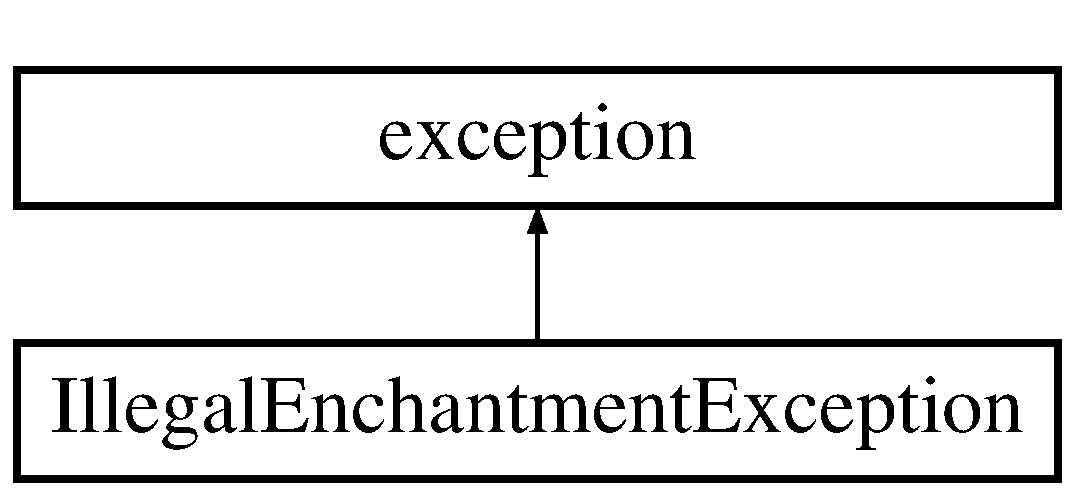
\includegraphics[height=2.000000cm]{class_illegal_enchantment_exception}
\end{center}
\end{figure}
\subsection*{Public Member Functions}
\begin{DoxyCompactItemize}
\item 
\hypertarget{class_illegal_enchantment_exception_a0a7c2474b42ba67341d836f98e287480}{}\label{class_illegal_enchantment_exception_a0a7c2474b42ba67341d836f98e287480} 
{\bfseries Illegal\+Enchantment\+Exception} (const std\+::string item\+Name, const std\+::string type\+Name, const std\+::string enchantment\+Name)
\item 
\hypertarget{class_illegal_enchantment_exception_a4a23145dda73d4563832d90bcfe7c684}{}\label{class_illegal_enchantment_exception_a4a23145dda73d4563832d90bcfe7c684} 
virtual const char $\ast$ {\bfseries what} () const  throw ()
\end{DoxyCompactItemize}


\subsection{Detailed Description}


Definition at line 11 of file inventory\+\_\+exceptions.\+h.



The documentation for this class was generated from the following file\+:\begin{DoxyCompactItemize}
\item 
inventory\+\_\+exceptions.\+h\end{DoxyCompactItemize}

\hypertarget{class_inventory}{}\section{Inventory Class Reference}
\label{class_inventory}\index{Inventory@{Inventory}}
\subsection*{Public Member Functions}
\begin{DoxyCompactItemize}
\item 
\hypertarget{class_inventory_a804c8fd9e053eece373af66a394c20e6}{}\label{class_inventory_a804c8fd9e053eece373af66a394c20e6} 
void {\bfseries update\+Lvl} (int a\+Level)
\item 
\hypertarget{class_inventory_aaf1dd5cdc379114db88ddb6efb8824ec}{}\label{class_inventory_aaf1dd5cdc379114db88ddb6efb8824ec} 
\hyperlink{class_item}{Item} $\ast$ {\bfseries get\+Equip\+Type} (\hyperlink{class_equip_type}{Equip\+Type} an\+Equip)
\item 
\hypertarget{class_inventory_acc4bbbe2553b7a6dc50ec9e1fe9a3ea2}{}\label{class_inventory_acc4bbbe2553b7a6dc50ec9e1fe9a3ea2} 
\hyperlink{class_equipment}{Equipment} {\bfseries get\+Equipment} (\hyperlink{class_equip_type}{Equip\+Type} a\+Type)
\item 
\hypertarget{class_inventory_a8b886a0ab6b3b14ee3b1a0f3e12155ef}{}\label{class_inventory_a8b886a0ab6b3b14ee3b1a0f3e12155ef} 
int $\ast$ {\bfseries get\+All\+Equip\+Mods} ()
\item 
\hypertarget{class_inventory_a79bf7166e4d63954092137e3ae3c3780}{}\label{class_inventory_a79bf7166e4d63954092137e3ae3c3780} 
int {\bfseries get\+Equip\+Mod} (\hyperlink{class_ability}{Ability} abl)
\item 
\hypertarget{class_inventory_abdaf4c69012ccbece97c87fa169c6648}{}\label{class_inventory_abdaf4c69012ccbece97c87fa169c6648} 
int {\bfseries get\+Equip\+Mod} (int index)
\item 
\hypertarget{class_inventory_a83af81c1871295b5a4e87b8372db577a}{}\label{class_inventory_a83af81c1871295b5a4e87b8372db577a} 
int {\bfseries get\+Weight} ()
\item 
\hypertarget{class_inventory_a666f1f8c42d652235210f8199c586e74}{}\label{class_inventory_a666f1f8c42d652235210f8199c586e74} 
unordered\+\_\+set$<$ \hyperlink{class_item}{Item} $\ast$ $>$ {\bfseries get\+Back\+Pack} ()
\item 
\hypertarget{class_inventory_a8c841bce89b1a4958f22dee158bafccf}{}\label{class_inventory_a8c841bce89b1a4958f22dee158bafccf} 
bool {\bfseries add\+To\+Pack} (\hyperlink{class_item}{Item} $\ast$an\+Item)
\item 
\hypertarget{class_inventory_a061ffa9b738372bfcaee6d8ea5140d05}{}\label{class_inventory_a061ffa9b738372bfcaee6d8ea5140d05} 
void {\bfseries remove\+From\+Pack} (\hyperlink{class_item}{Item} $\ast$an\+Item)
\item 
\hypertarget{class_inventory_a7d9e9f5217573c9052484543e481ead1}{}\label{class_inventory_a7d9e9f5217573c9052484543e481ead1} 
bool {\bfseries equip} (\hyperlink{class_equipment}{Equipment} $\ast$an\+Item)
\item 
\hypertarget{class_inventory_aa5cd8a3fd8309a9f2a23b595b24b6fb5}{}\label{class_inventory_aa5cd8a3fd8309a9f2a23b595b24b6fb5} 
bool {\bfseries unequip} (\hyperlink{class_equip_type}{Equip\+Type} a\+Type)
\item 
\hypertarget{class_inventory_a061da226215e169d1b9f0c05e9d84a1d}{}\label{class_inventory_a061da226215e169d1b9f0c05e9d84a1d} 
std\+::unordered\+\_\+set$<$ \hyperlink{class_key_item}{Key\+Item} $\ast$ $>$ {\bfseries key\+Chain} ()
\item 
\hypertarget{class_inventory_aa9cfa40da293bf94acc9f0c8fbe9a7d1}{}\label{class_inventory_aa9cfa40da293bf94acc9f0c8fbe9a7d1} 
std\+::string {\bfseries to\+String} ()
\end{DoxyCompactItemize}
\subsection*{Friends}
\begin{DoxyCompactItemize}
\item 
\hypertarget{class_inventory_ac98d07dd8f7b70e16ccb9a01abf56b9c}{}\label{class_inventory_ac98d07dd8f7b70e16ccb9a01abf56b9c} 
class {\bfseries boost\+::serialization\+::access}
\end{DoxyCompactItemize}


\subsection{Detailed Description}


Definition at line 341 of file inv2.\+h.



The documentation for this class was generated from the following files\+:\begin{DoxyCompactItemize}
\item 
inv2.\+h\item 
inv2.\+cpp\end{DoxyCompactItemize}

\hypertarget{class_item}{}\section{Item Class Reference}
\label{class_item}\index{Item@{Item}}
Inheritance diagram for Item\+:\begin{figure}[H]
\begin{center}
\leavevmode
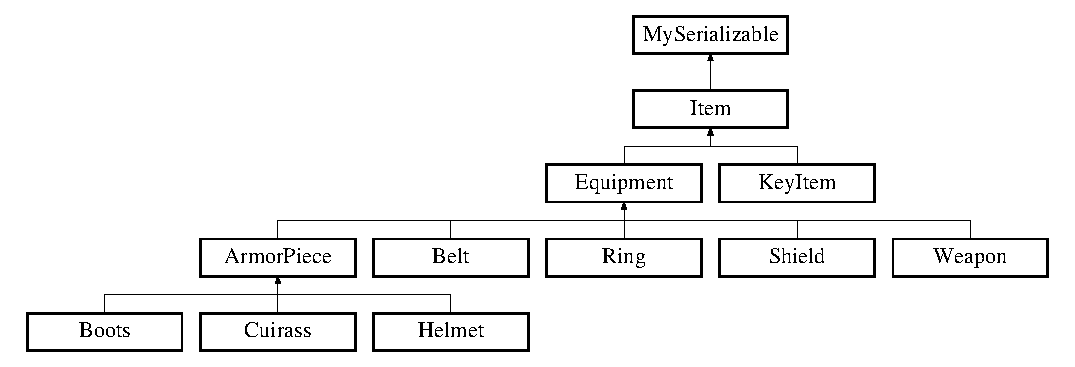
\includegraphics[height=4.487180cm]{class_item}
\end{center}
\end{figure}
\subsection*{Public Member Functions}
\begin{DoxyCompactItemize}
\item 
\hypertarget{class_item_a63d7f2148b699e539aae354b01559811}{}\label{class_item_a63d7f2148b699e539aae354b01559811} 
string {\bfseries get\+Name} ()
\item 
\hypertarget{class_item_a8d2b9d404f8e692f456af88a1eb1ce44}{}\label{class_item_a8d2b9d404f8e692f456af88a1eb1ce44} 
string {\bfseries get\+Name} () const
\item 
\hypertarget{class_item_a49bc6fcbaf2e8e6695ad22408adedf5e}{}\label{class_item_a49bc6fcbaf2e8e6695ad22408adedf5e} 
virtual std\+::string {\bfseries get\+Class\+Name} ()
\item 
\hypertarget{class_item_a1350dcc7942c35ddc6dc4bf646e8c663}{}\label{class_item_a1350dcc7942c35ddc6dc4bf646e8c663} 
virtual std\+::string {\bfseries get\+Class\+Name} () const
\item 
\hypertarget{class_item_ae1461c50b7b64395132317e24027dc08}{}\label{class_item_ae1461c50b7b64395132317e24027dc08} 
virtual void {\bfseries update\+Lvl} (int player\+Level)
\item 
\hypertarget{class_item_a96cce91c32165e1ed182138930ccb751}{}\label{class_item_a96cce91c32165e1ed182138930ccb751} 
bool {\bfseries reset} ()
\item 
\hypertarget{class_item_a3e358c86a1c658109eb797476051a1d6}{}\label{class_item_a3e358c86a1c658109eb797476051a1d6} 
virtual void {\bfseries save} (std\+::string filename)
\item 
\hypertarget{class_item_a9b426ccb054272b8059ba53923a61bd7}{}\label{class_item_a9b426ccb054272b8059ba53923a61bd7} 
virtual void {\bfseries load} (std\+::string filename)
\item 
\hypertarget{class_item_ac6e6f565235b7f7a6150a8dcf57ed66a}{}\label{class_item_ac6e6f565235b7f7a6150a8dcf57ed66a} 
virtual std\+::string {\bfseries to\+String} ()
\end{DoxyCompactItemize}
\subsection*{Protected Member Functions}
\begin{DoxyCompactItemize}
\item 
\hypertarget{class_item_a98956a129a5a3c47ac8466306090df0c}{}\label{class_item_a98956a129a5a3c47ac8466306090df0c} 
{\bfseries Item} (std\+::string a\+Name)
\end{DoxyCompactItemize}
\subsection*{Friends}
\begin{DoxyCompactItemize}
\item 
\hypertarget{class_item_ac98d07dd8f7b70e16ccb9a01abf56b9c}{}\label{class_item_ac98d07dd8f7b70e16ccb9a01abf56b9c} 
class {\bfseries boost\+::serialization\+::access}
\end{DoxyCompactItemize}


\subsection{Detailed Description}


Definition at line 21 of file inv2.\+h.



The documentation for this class was generated from the following file\+:\begin{DoxyCompactItemize}
\item 
inv2.\+h\end{DoxyCompactItemize}

\hypertarget{class_item_comparator}{}\section{Item\+Comparator Class Reference}
\label{class_item_comparator}\index{Item\+Comparator@{Item\+Comparator}}
\subsection*{Public Member Functions}
\begin{DoxyCompactItemize}
\item 
\hypertarget{class_item_comparator_aed204fa45ce29576828361be79c016ec}{}\label{class_item_comparator_aed204fa45ce29576828361be79c016ec} 
bool {\bfseries operator()} (const \hyperlink{class_item}{Item} \&item1, const \hyperlink{class_item}{Item} \&item2)
\end{DoxyCompactItemize}


\subsection{Detailed Description}


Definition at line 58 of file inv2.\+h.



The documentation for this class was generated from the following file\+:\begin{DoxyCompactItemize}
\item 
inv2.\+h\end{DoxyCompactItemize}

\hypertarget{class_key_item}{}\section{Key\+Item Class Reference}
\label{class_key_item}\index{Key\+Item@{Key\+Item}}


{\ttfamily \#include $<$inv2.\+h$>$}

Inheritance diagram for Key\+Item\+:\begin{figure}[H]
\begin{center}
\leavevmode
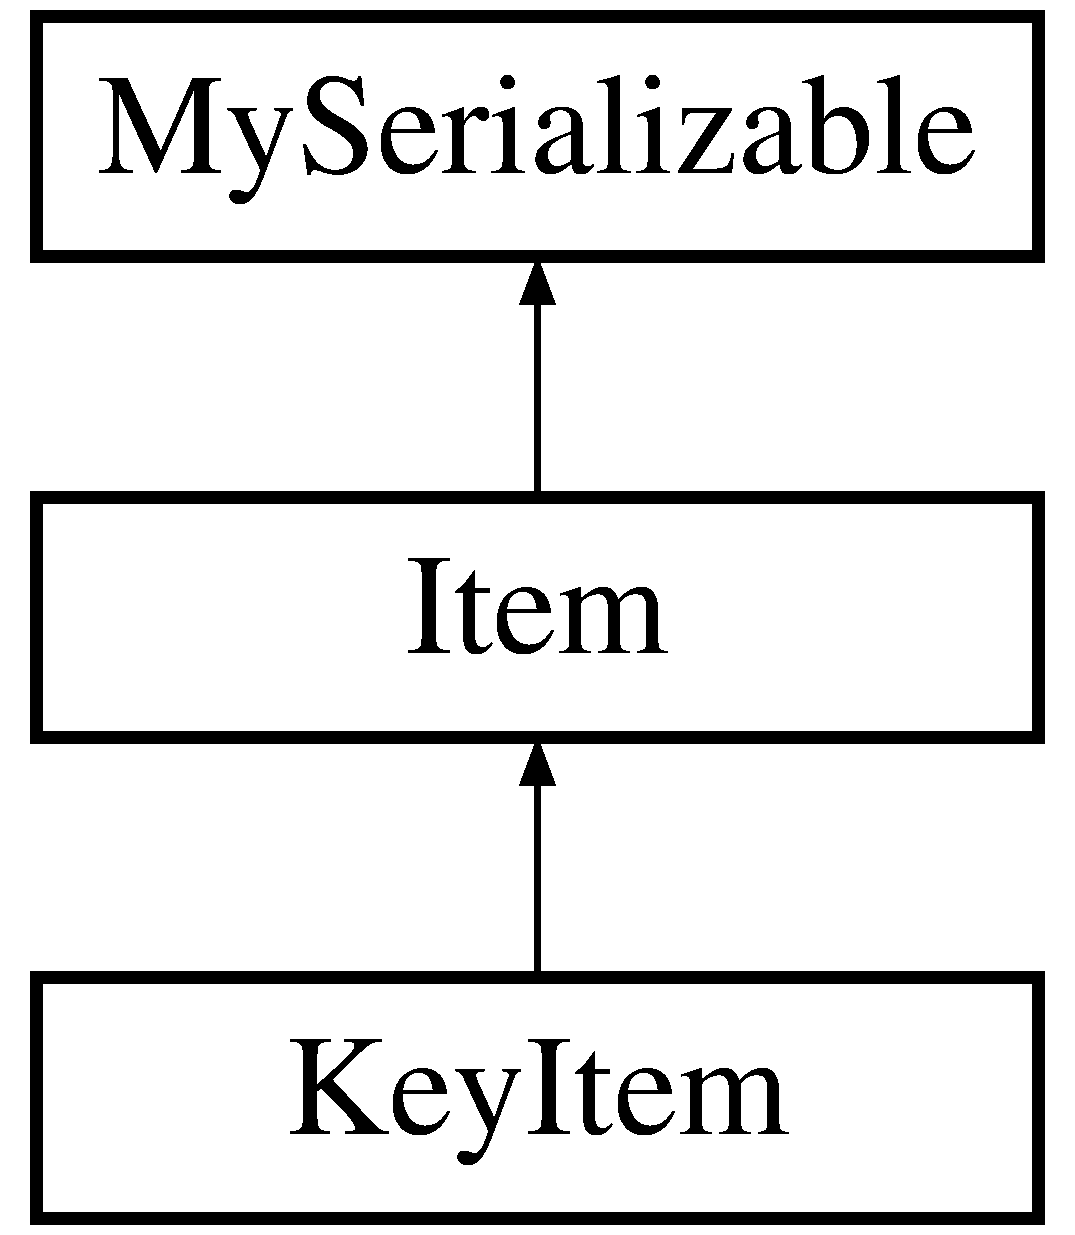
\includegraphics[height=3.000000cm]{class_key_item}
\end{center}
\end{figure}
\subsection*{Public Member Functions}
\begin{DoxyCompactItemize}
\item 
\hypertarget{class_key_item_aa0baded1e424eb98bfd44a02b69cc09a}{}\label{class_key_item_aa0baded1e424eb98bfd44a02b69cc09a} 
{\bfseries Key\+Item} (std\+::string a\+Name, int a\+Code)
\item 
\hypertarget{class_key_item_a3b9afd2ff4fc063a2821fa8fe4427fce}{}\label{class_key_item_a3b9afd2ff4fc063a2821fa8fe4427fce} 
int {\bfseries get\+Code} ()
\item 
\hypertarget{class_key_item_a9cf93545aaadfe60b3ca76c557acc38a}{}\label{class_key_item_a9cf93545aaadfe60b3ca76c557acc38a} 
virtual void {\bfseries save} (std\+::string filename)
\item 
\hypertarget{class_key_item_ae589a39407c4fd6ff1a9086693665532}{}\label{class_key_item_ae589a39407c4fd6ff1a9086693665532} 
virtual void {\bfseries load} (std\+::string filename)
\end{DoxyCompactItemize}
\subsection*{Static Public Member Functions}
\begin{DoxyCompactItemize}
\item 
\hypertarget{class_key_item_a853eded6ba25adb28a34020285ee0e7e}{}\label{class_key_item_a853eded6ba25adb28a34020285ee0e7e} 
static \hyperlink{class_key_item}{Key\+Item} {\bfseries s\+Load} (std\+::string filename)
\end{DoxyCompactItemize}
\subsection*{Friends}
\begin{DoxyCompactItemize}
\item 
\hypertarget{class_key_item_ac98d07dd8f7b70e16ccb9a01abf56b9c}{}\label{class_key_item_ac98d07dd8f7b70e16ccb9a01abf56b9c} 
class {\bfseries boost\+::serialization\+::access}
\end{DoxyCompactItemize}
\subsection*{Additional Inherited Members}


\subsection{Detailed Description}
Key item to unlock a \hyperlink{class_lockable}{Lockable} item (chest, door) Derives \hyperlink{class_item}{Item} 

Definition at line 312 of file inv2.\+h.



The documentation for this class was generated from the following files\+:\begin{DoxyCompactItemize}
\item 
inv2.\+h\item 
inv2.\+cpp\end{DoxyCompactItemize}

\hypertarget{class_lockable}{}\section{Lockable Class Reference}
\label{class_lockable}\index{Lockable@{Lockable}}
Inheritance diagram for Lockable\+:\begin{figure}[H]
\begin{center}
\leavevmode
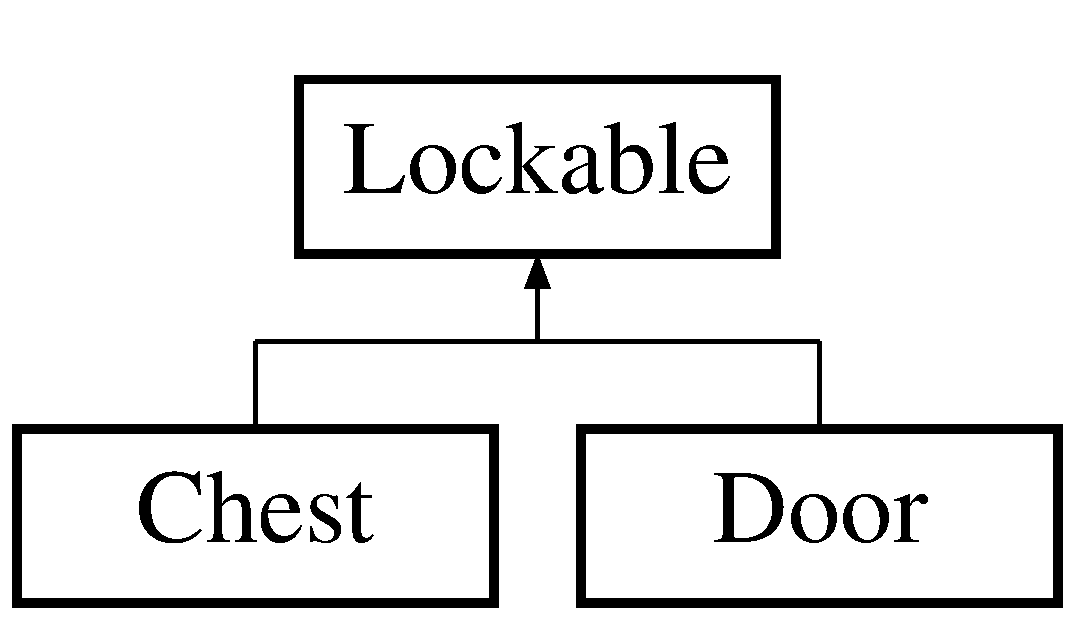
\includegraphics[height=2.000000cm]{class_lockable}
\end{center}
\end{figure}
\subsection*{Public Member Functions}
\begin{DoxyCompactItemize}
\item 
\hypertarget{class_lockable_a41cbb1a47f33edbba4e7d8addf464102}{}\label{class_lockable_a41cbb1a47f33edbba4e7d8addf464102} 
\hyperlink{class_key_item}{Key\+Item} {\bfseries get\+Key} ()
\item 
\hypertarget{class_lockable_a6297adf59c34be6743690ffac934e1c3}{}\label{class_lockable_a6297adf59c34be6743690ffac934e1c3} 
int {\bfseries get\+Status} ()
\item 
\hypertarget{class_lockable_af1a63132342bc4bcb58d63f5ee4dc94a}{}\label{class_lockable_af1a63132342bc4bcb58d63f5ee4dc94a} 
void {\bfseries set\+Status} (int a\+Status)
\item 
\hypertarget{class_lockable_a99c6790e2b56bef4618a1f3a461b7c63}{}\label{class_lockable_a99c6790e2b56bef4618a1f3a461b7c63} 
int {\bfseries unlock} (\hyperlink{class_key_item}{Key\+Item} a\+Key)
\item 
\hypertarget{class_lockable_a5593ee3b706c7a47f0e0bc9035be3433}{}\label{class_lockable_a5593ee3b706c7a47f0e0bc9035be3433} 
int {\bfseries open} ()
\item 
\hypertarget{class_lockable_a7050cc99c85178d73aba1fe4c81161f5}{}\label{class_lockable_a7050cc99c85178d73aba1fe4c81161f5} 
bool {\bfseries is\+Locked} ()
\item 
\hypertarget{class_lockable_a3520cfcd7af2d8f3d2f5bb615be76f10}{}\label{class_lockable_a3520cfcd7af2d8f3d2f5bb615be76f10} 
bool {\bfseries is\+Open} ()
\item 
\hypertarget{class_lockable_a46cd55be38b7bd08e3fe5c39f80e412c}{}\label{class_lockable_a46cd55be38b7bd08e3fe5c39f80e412c} 
virtual std\+::string {\bfseries key\+Name} ()
\item 
\hypertarget{class_lockable_ad4bddb3c5f07a3a6130ac84810e67167}{}\label{class_lockable_ad4bddb3c5f07a3a6130ac84810e67167} 
void {\bfseries reset} ()
\end{DoxyCompactItemize}
\subsection*{Protected Member Functions}
\begin{DoxyCompactItemize}
\item 
\hypertarget{class_lockable_a77a726b41027e421f0735f546d667417}{}\label{class_lockable_a77a726b41027e421f0735f546d667417} 
{\bfseries Lockable} (std\+::string name)
\end{DoxyCompactItemize}
\subsection*{Friends}
\begin{DoxyCompactItemize}
\item 
\hypertarget{class_lockable_ac98d07dd8f7b70e16ccb9a01abf56b9c}{}\label{class_lockable_ac98d07dd8f7b70e16ccb9a01abf56b9c} 
class {\bfseries boost\+::serialization\+::access}
\end{DoxyCompactItemize}


\subsection{Detailed Description}


Definition at line 15 of file basic\+\_\+structure.\+h.



The documentation for this class was generated from the following files\+:\begin{DoxyCompactItemize}
\item 
basic\+\_\+structure.\+h\item 
basic\+\_\+structure.\+cpp\end{DoxyCompactItemize}

\hypertarget{class_map}{}\section{Map Class Reference}
\label{class_map}\index{Map@{Map}}


\hyperlink{class_map}{Map} object.  




{\ttfamily \#include $<$map.\+h$>$}

Inheritance diagram for Map\+:\begin{figure}[H]
\begin{center}
\leavevmode
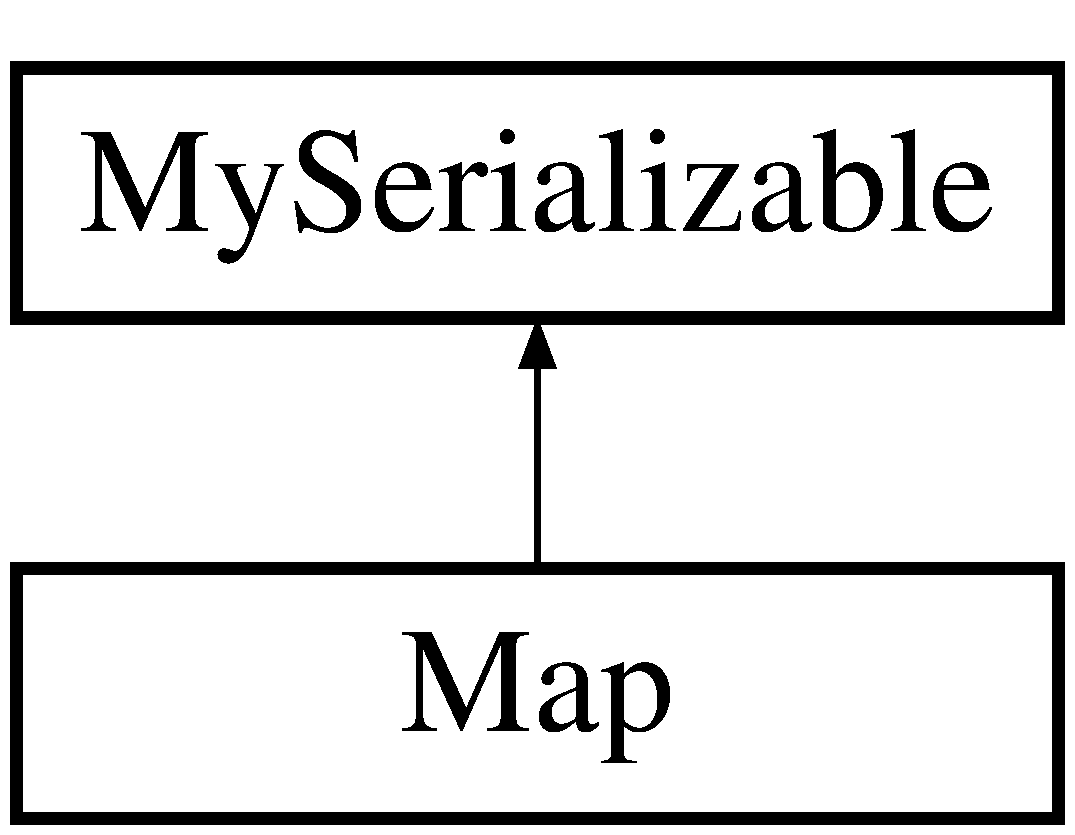
\includegraphics[height=2.000000cm]{class_map}
\end{center}
\end{figure}
\subsection*{Public Member Functions}
\begin{DoxyCompactItemize}
\item 
\hypertarget{class_map_ab98b96f44d9fef2a266556297cee71be}{}\label{class_map_ab98b96f44d9fef2a266556297cee71be} 
\hyperlink{class_map}{Map} {\bfseries s\+Load} (std\+::string filename)
\item 
\hyperlink{class_map_a0f5ad0fd4563497b4214038cbca8b582}{Map} ()
\begin{DoxyCompactList}\small\item\em Default constructor for a \hyperlink{class_map}{Map}. \end{DoxyCompactList}\item 
\hypertarget{class_map_a2edce4c7d4627d9f0ed6ae08021590ed}{}\label{class_map_a2edce4c7d4627d9f0ed6ae08021590ed} 
{\bfseries Map} (std\+::string a\+Name, int h, int w)
\item 
\hypertarget{class_map_aa403fbe09394ccf39747588f5168e3b2}{}\label{class_map_aa403fbe09394ccf39747588f5168e3b2} 
\hyperlink{class_map_aa403fbe09394ccf39747588f5168e3b2}{$\sim$\+Map} ()
\begin{DoxyCompactList}\small\item\em \hyperlink{class_map}{Map} destructor. \end{DoxyCompactList}\item 
\hypertarget{class_map_a904c445fdce79257fedeba09070cf88a}{}\label{class_map_a904c445fdce79257fedeba09070cf88a} 
void {\bfseries reset} ()
\item 
\hypertarget{class_map_af7c347ec2e29fc7b97c81730f94176f2}{}\label{class_map_af7c347ec2e29fc7b97c81730f94176f2} 
bool {\bfseries start} (\hyperlink{class_player}{Player} $\ast$a\+Player)
\item 
\hypertarget{class_map_ab22dc646bc833bb6b4070dcc2d3bd7c0}{}\label{class_map_ab22dc646bc833bb6b4070dcc2d3bd7c0} 
bool {\bfseries cell\+Exists} (int row, int col)
\item 
\hypertarget{class_map_afd34d12227676b3cebeed9f5fae2508f}{}\label{class_map_afd34d12227676b3cebeed9f5fae2508f} 
int {\bfseries get\+Width} ()
\item 
\hypertarget{class_map_a2b09c8875af2efb711fc3a022e70427d}{}\label{class_map_a2b09c8875af2efb711fc3a022e70427d} 
int {\bfseries get\+Height} ()
\item 
\hypertarget{class_map_ac031089e3376749c6a9b97d0cce8c598}{}\label{class_map_ac031089e3376749c6a9b97d0cce8c598} 
void {\bfseries set\+Name} (std\+::string a\+Name)
\item 
\hypertarget{class_map_a67432b1e7f5ab087a75a74e2dd6589ec}{}\label{class_map_a67432b1e7f5ab087a75a74e2dd6589ec} 
std\+::string {\bfseries get\+Name} ()
\item 
\hypertarget{class_map_afc1c246f4bc6bde164ac2dafa79bf5fb}{}\label{class_map_afc1c246f4bc6bde164ac2dafa79bf5fb} 
\hyperlink{class_cell}{Cell} $\ast$ \hyperlink{class_map_afc1c246f4bc6bde164ac2dafa79bf5fb}{get\+Cell} (int row, int col)
\begin{DoxyCompactList}\small\item\em Function that returns a pointer to a board \hyperlink{class_cell}{Cell}. \end{DoxyCompactList}\item 
\hypertarget{class_map_a26b8b9bc68f8f7e5b4f74cbd3210dd30}{}\label{class_map_a26b8b9bc68f8f7e5b4f74cbd3210dd30} 
void {\bfseries clear\+Cell} (int row, int col)
\item 
\hypertarget{class_map_a502496d0178402534ec6701d10bbb0e6}{}\label{class_map_a502496d0178402534ec6701d10bbb0e6} 
bool {\bfseries add\+Stop} (int row, int col, int position)
\item 
\hypertarget{class_map_a382d1000a33c473bd96a619a0dd11d16}{}\label{class_map_a382d1000a33c473bd96a619a0dd11d16} 
bool {\bfseries update\+First\+Stop} (int row, int col)
\item 
\hypertarget{class_map_a0320959aa6cdae5dfe4cff3f79ebd40a}{}\label{class_map_a0320959aa6cdae5dfe4cff3f79ebd40a} 
bool {\bfseries update\+Last\+Stop} (int row, int col)
\item 
\hypertarget{class_map_a808119272b760e43615ffc396cf6feb6}{}\label{class_map_a808119272b760e43615ffc396cf6feb6} 
bool {\bfseries remove\+Stop} (int row, int col, int position)
\item 
\hypertarget{class_map_a9f10c89830337667bc392e3814b5e616}{}\label{class_map_a9f10c89830337667bc392e3814b5e616} 
bool {\bfseries add\+To\+Cell} (\hyperlink{class_placeable}{Placeable} $\ast$to\+Place, int row, int col)
\item 
bool \hyperlink{class_map_a7b5c1d8ed873a72484f27e99bcdff97a}{set\+Row\+Wall} (int row, int from, int end)
\begin{DoxyCompactList}\small\item\em Mehtod that instantiate \hyperlink{class_wall}{Wall} objects in a horizontal range \hyperlink{class_cell}{Cell}. \end{DoxyCompactList}\item 
bool \hyperlink{class_map_a7e89d11a89a796ac46e60722533f23d4}{set\+Col\+Wall} (int col, int from, int end)
\begin{DoxyCompactList}\small\item\em Mehtod that instantiate \hyperlink{class_wall}{Wall} objects in a vertical range \hyperlink{class_cell}{Cell}. \end{DoxyCompactList}\item 
\hypertarget{class_map_a9c37a12b6aa0fcf4f849a706c4cd2598}{}\label{class_map_a9c37a12b6aa0fcf4f849a706c4cd2598} 
bool {\bfseries move} (int b\+Row, int b\+Col, int e\+Row, int e\+Col)
\item 
\hypertarget{class_map_af9b2cb5b80f93e05fe94d24f0cd0b4d0}{}\label{class_map_af9b2cb5b80f93e05fe94d24f0cd0b4d0} 
bool {\bfseries move} (int b\+Row, int b\+Col, \hyperlink{class_direction}{Direction} dir)
\item 
\hypertarget{class_map_a22641b39f3eadb59771d2e5d02ff19c3}{}\label{class_map_a22641b39f3eadb59771d2e5d02ff19c3} 
bool {\bfseries move} (\hyperlink{class_cell}{Cell} $\ast$from, \hyperlink{class_direction}{Direction} dir)
\item 
\hypertarget{class_map_ad1af1c1145fbc4675952fa10c0aacf61}{}\label{class_map_ad1af1c1145fbc4675952fa10c0aacf61} 
bool {\bfseries valid\+Path} ()
\item 
\hypertarget{class_map_a6749a0b9a270aef552af6bd94f88e7bc}{}\label{class_map_a6749a0b9a270aef552af6bd94f88e7bc} 
bool {\bfseries valid\+Path} (int begin\+Row, int begin\+Col, int exit\+Row, int exit\+Col)
\item 
\hypertarget{class_map_aeb226f399e3e44cc5ecb100b4c378848}{}\label{class_map_aeb226f399e3e44cc5ecb100b4c378848} 
int $\ast$$\ast$ {\bfseries dijkstra} (int const exit\+Row, int const exit\+Col)
\item 
\hypertarget{class_map_aa9ac575aa037a6d8ed05eb4c36bb66c1}{}\label{class_map_aa9ac575aa037a6d8ed05eb4c36bb66c1} 
int $\ast$$\ast$ {\bfseries dijkstra} (\hyperlink{class_cell}{Cell} $\ast$reference)
\item 
\hypertarget{class_map_a76ba15e9f73cfdf657e00720744b4466}{}\label{class_map_a76ba15e9f73cfdf657e00720744b4466} 
bool {\bfseries operator==} (\hyperlink{class_map}{Map} \&const rhs\+Map)
\item 
\hypertarget{class_map_a13a2dfbee73ab704f06d9a6cf153beb6}{}\label{class_map_a13a2dfbee73ab704f06d9a6cf153beb6} 
bool {\bfseries operator!=} (\hyperlink{class_map}{Map} \&const rhs\+Map)
\item 
\hypertarget{class_map_af7b0ff0228286f88cd6b6a2b87604004}{}\label{class_map_af7b0ff0228286f88cd6b6a2b87604004} 
void {\bfseries load} (std\+::string filename)
\item 
\hypertarget{class_map_a0b67e2b03238fd18ecab89d8369ca67b}{}\label{class_map_a0b67e2b03238fd18ecab89d8369ca67b} 
void {\bfseries save} (std\+::string filename)
\item 
\hypertarget{class_map_a8f2e95c92c3b1b36d9212b101d755bd8}{}\label{class_map_a8f2e95c92c3b1b36d9212b101d755bd8} 
vector$<$ \hyperlink{class_cell}{Cell} $\ast$ $>$ {\bfseries operator\mbox{[}$\,$\mbox{]}} (int i)
\item 
\hypertarget{class_map_a94c656e72ab63c3791c1f8522f56f603}{}\label{class_map_a94c656e72ab63c3791c1f8522f56f603} 
std\+::string {\bfseries to\+String} ()
\end{DoxyCompactItemize}
\subsection*{Static Public Member Functions}
\begin{DoxyCompactItemize}
\item 
\hypertarget{class_map_a5862ce4a3b20cb267fc19d4167aa3f05}{}\label{class_map_a5862ce4a3b20cb267fc19d4167aa3f05} 
static const int $\ast$$\ast$ {\bfseries get\+Distance\+Graph} (int const exit\+Row, int const exit\+Col)
\end{DoxyCompactItemize}
\subsection*{Friends}
\begin{DoxyCompactItemize}
\item 
\hypertarget{class_map_ac98d07dd8f7b70e16ccb9a01abf56b9c}{}\label{class_map_ac98d07dd8f7b70e16ccb9a01abf56b9c} 
class {\bfseries boost\+::serialization\+::access}
\end{DoxyCompactItemize}


\subsection{Detailed Description}
\hyperlink{class_map}{Map} object. 

Definition at line 43 of file map.\+h.



\subsection{Constructor \& Destructor Documentation}
\hypertarget{class_map_a0f5ad0fd4563497b4214038cbca8b582}{}\label{class_map_a0f5ad0fd4563497b4214038cbca8b582} 
\index{Map@{Map}!Map@{Map}}
\index{Map@{Map}!Map@{Map}}
\subsubsection{\texorpdfstring{Map()}{Map()}}
{\footnotesize\ttfamily Map\+::\+Map (\begin{DoxyParamCaption}{ }\end{DoxyParamCaption})}



Default constructor for a \hyperlink{class_map}{Map}. 

initializes a blank \hyperlink{class_map}{Map} of size 10 x 10. 

Definition at line 16 of file map.\+cpp.


\begin{DoxyCode}
16          : height(5), width(5),
17 board(vector<vector<Cell*>>()),
18 stops(std::list<Cell*>())
19 \{
20     initMap();
21     stops.push\_front((*\textcolor{keyword}{this})[0][0]);
22     stops.push\_back(\hyperlink{class_map_afc1c246f4bc6bde164ac2dafa79bf5fb}{getCell}(this->getHeight() - 1, this->getWidth() - 1));
23 \}
\end{DoxyCode}


\subsection{Member Function Documentation}
\hypertarget{class_map_a7e89d11a89a796ac46e60722533f23d4}{}\label{class_map_a7e89d11a89a796ac46e60722533f23d4} 
\index{Map@{Map}!set\+Col\+Wall@{set\+Col\+Wall}}
\index{set\+Col\+Wall@{set\+Col\+Wall}!Map@{Map}}
\subsubsection{\texorpdfstring{set\+Col\+Wall()}{setColWall()}}
{\footnotesize\ttfamily bool Map\+::set\+Col\+Wall (\begin{DoxyParamCaption}\item[{int}]{col,  }\item[{int}]{start,  }\item[{int}]{end }\end{DoxyParamCaption})}



Mehtod that instantiate \hyperlink{class_wall}{Wall} objects in a vertical range \hyperlink{class_cell}{Cell}. 


\begin{DoxyParams}{Parameters}
{\em col} & the index of the col to set the \hyperlink{class_wall}{Wall} in. \\
\hline
{\em start} & the index of the cell at which to start the \hyperlink{class_wall}{Wall}. \\
\hline
{\em end} & the index of the \hyperlink{class_cell}{Cell} at which to end the \hyperlink{class_wall}{Wall}. \\
\hline
\end{DoxyParams}


Definition at line 270 of file map.\+cpp.


\begin{DoxyCode}
271 \{
272     \textcolor{keywordtype}{int} i;
273 
274     \textcolor{keywordflow}{if} (cellExists(start, col) && cellExists(end, col))
275     \{
276 
277         \textcolor{keywordflow}{for} (i = start; i < this->getHeight() && i <= end; i++)
278         \{
279             \textcolor{keywordflow}{return} board[i][col]->setContent(\textcolor{keyword}{new} \hyperlink{class_wall}{Wall}());
280         \}
281 
282         \textcolor{keywordflow}{return} \textcolor{keyword}{true};
283     \}
284 
285     \textcolor{keywordflow}{return} \textcolor{keyword}{false};
286 \}
\end{DoxyCode}
\hypertarget{class_map_a7b5c1d8ed873a72484f27e99bcdff97a}{}\label{class_map_a7b5c1d8ed873a72484f27e99bcdff97a} 
\index{Map@{Map}!set\+Row\+Wall@{set\+Row\+Wall}}
\index{set\+Row\+Wall@{set\+Row\+Wall}!Map@{Map}}
\subsubsection{\texorpdfstring{set\+Row\+Wall()}{setRowWall()}}
{\footnotesize\ttfamily bool Map\+::set\+Row\+Wall (\begin{DoxyParamCaption}\item[{int}]{row,  }\item[{int}]{start,  }\item[{int}]{end }\end{DoxyParamCaption})}



Mehtod that instantiate \hyperlink{class_wall}{Wall} objects in a horizontal range \hyperlink{class_cell}{Cell}. 


\begin{DoxyParams}{Parameters}
{\em row} & the index of the row to set the \hyperlink{class_wall}{Wall} in. \\
\hline
{\em start} & the index of the cell at which to start the \hyperlink{class_wall}{Wall}. \\
\hline
{\em end} & the index of the \hyperlink{class_cell}{Cell} at which to end the \hyperlink{class_wall}{Wall}. \\
\hline
\end{DoxyParams}


Definition at line 250 of file map.\+cpp.


\begin{DoxyCode}
251 \{
252     \textcolor{keywordtype}{int} j;
253 
254     \textcolor{keywordflow}{if} (cellExists(row, start) && cellExists(row, end))
255     \{
256 
257         \textcolor{keywordflow}{for} (j = start; j < this->getWidth() && j <= end; j++)
258         \{
259             \textcolor{keywordflow}{return} board[row][j]->setContent(\textcolor{keyword}{new} \hyperlink{class_wall}{Wall}());
260         \}
261     \}
262 
263     \textcolor{keywordflow}{return} \textcolor{keyword}{false};
264 \}
\end{DoxyCode}


The documentation for this class was generated from the following files\+:\begin{DoxyCompactItemize}
\item 
map.\+h\item 
map.\+cpp\end{DoxyCompactItemize}

\hypertarget{class_my_serializable}{}\section{My\+Serializable Class Reference}
\label{class_my_serializable}\index{My\+Serializable@{My\+Serializable}}
Inheritance diagram for My\+Serializable\+:\begin{figure}[H]
\begin{center}
\leavevmode
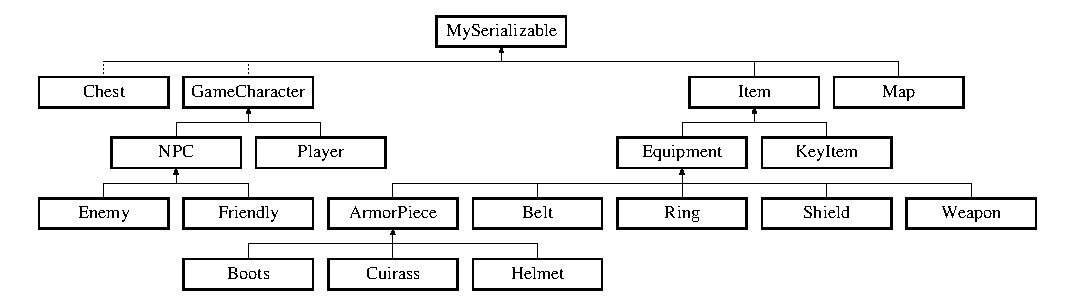
\includegraphics[height=3.669725cm]{class_my_serializable}
\end{center}
\end{figure}
\subsection*{Public Member Functions}
\begin{DoxyCompactItemize}
\item 
\hypertarget{class_my_serializable_aecba7b7a0a257f15ccd42bcd7c320069}{}\label{class_my_serializable_aecba7b7a0a257f15ccd42bcd7c320069} 
virtual void {\bfseries save} (std\+::string filename)=0
\item 
\hypertarget{class_my_serializable_afa91367dc4d5606c1d62f5c50636e171}{}\label{class_my_serializable_afa91367dc4d5606c1d62f5c50636e171} 
virtual void {\bfseries load} (std\+::string filename)=0
\end{DoxyCompactItemize}
\subsection*{Friends}
\begin{DoxyCompactItemize}
\item 
\hypertarget{class_my_serializable_ac98d07dd8f7b70e16ccb9a01abf56b9c}{}\label{class_my_serializable_ac98d07dd8f7b70e16ccb9a01abf56b9c} 
class {\bfseries boost\+::serialization\+::access}
\end{DoxyCompactItemize}


\subsection{Detailed Description}


Definition at line 13 of file serializable.\+h.



The documentation for this class was generated from the following file\+:\begin{DoxyCompactItemize}
\item 
serializable.\+h\end{DoxyCompactItemize}

\hypertarget{class_n_p_c}{}\section{N\+PC Class Reference}
\label{class_n_p_c}\index{N\+PC@{N\+PC}}
Inheritance diagram for N\+PC\+:\begin{figure}[H]
\begin{center}
\leavevmode
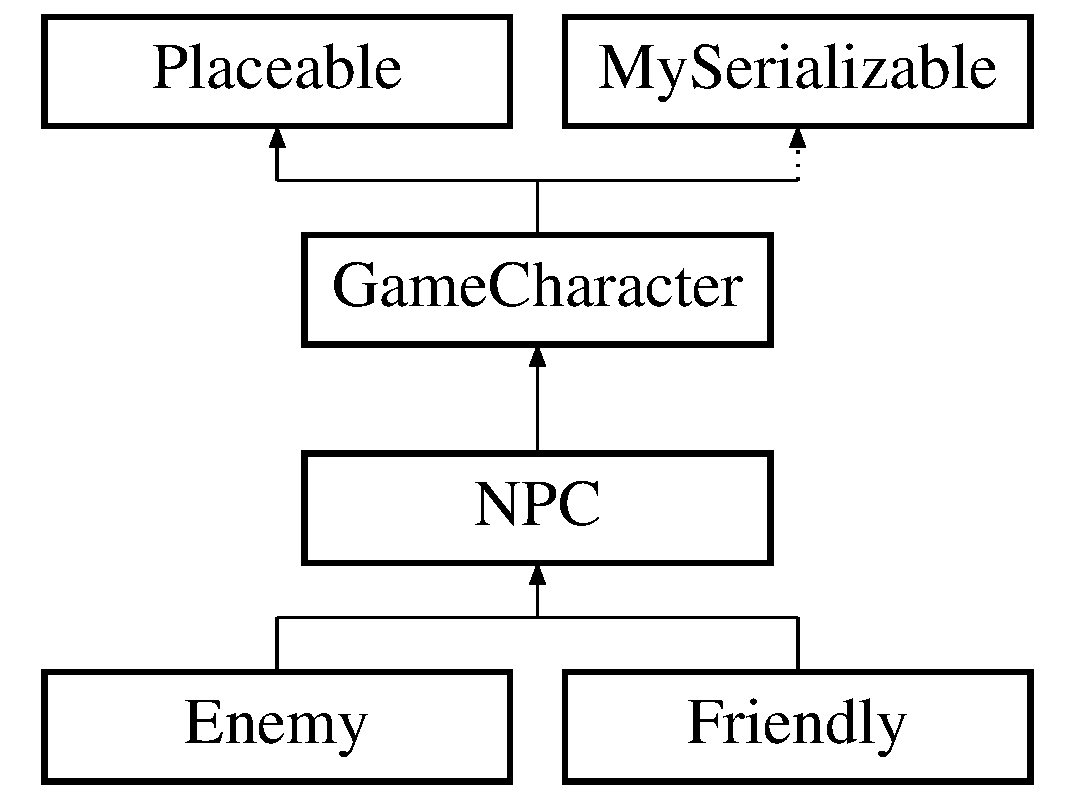
\includegraphics[height=4.000000cm]{class_n_p_c}
\end{center}
\end{figure}
\subsection*{Public Member Functions}
\begin{DoxyCompactItemize}
\item 
\hypertarget{class_n_p_c_ad33bef700a6b0b6d5619dc8af4e9ac62}{}\label{class_n_p_c_ad33bef700a6b0b6d5619dc8af4e9ac62} 
{\bfseries N\+PC} (std\+::string a\+Name, int a\+Level)
\item 
\hypertarget{class_n_p_c_a7e81f8ecedc0eb22349a68cd224dbc23}{}\label{class_n_p_c_a7e81f8ecedc0eb22349a68cd224dbc23} 
const char {\bfseries get\+Symbol} ()
\item 
\hypertarget{class_n_p_c_a90707f8d4132352e3a79f1774df9a3aa}{}\label{class_n_p_c_a90707f8d4132352e3a79f1774df9a3aa} 
bool {\bfseries reset} ()
\item 
\hypertarget{class_n_p_c_afd87c014b5c0d6d4404e9b1fa0ab35fa}{}\label{class_n_p_c_afd87c014b5c0d6d4404e9b1fa0ab35fa} 
virtual void {\bfseries get\+Strategy} ()
\item 
\hypertarget{class_n_p_c_a09d4b4500a23e4919915ba60682f2d20}{}\label{class_n_p_c_a09d4b4500a23e4919915ba60682f2d20} 
virtual void {\bfseries load} (std\+::string filename)
\item 
\hypertarget{class_n_p_c_a2ac4ef18f0adffd50ec066347ed027a6}{}\label{class_n_p_c_a2ac4ef18f0adffd50ec066347ed027a6} 
virtual void {\bfseries save} (std\+::string filename)
\end{DoxyCompactItemize}
\subsection*{Friends}
\begin{DoxyCompactItemize}
\item 
\hypertarget{class_n_p_c_ac98d07dd8f7b70e16ccb9a01abf56b9c}{}\label{class_n_p_c_ac98d07dd8f7b70e16ccb9a01abf56b9c} 
class {\bfseries boost\+::serialization\+::access}
\end{DoxyCompactItemize}


\subsection{Detailed Description}


Definition at line 132 of file character.\+h.



The documentation for this class was generated from the following files\+:\begin{DoxyCompactItemize}
\item 
character.\+h\item 
character.\+cpp\end{DoxyCompactItemize}

\hypertarget{class_placeable}{}\section{Placeable Class Reference}
\label{class_placeable}\index{Placeable@{Placeable}}
Inheritance diagram for Placeable\+:\begin{figure}[H]
\begin{center}
\leavevmode
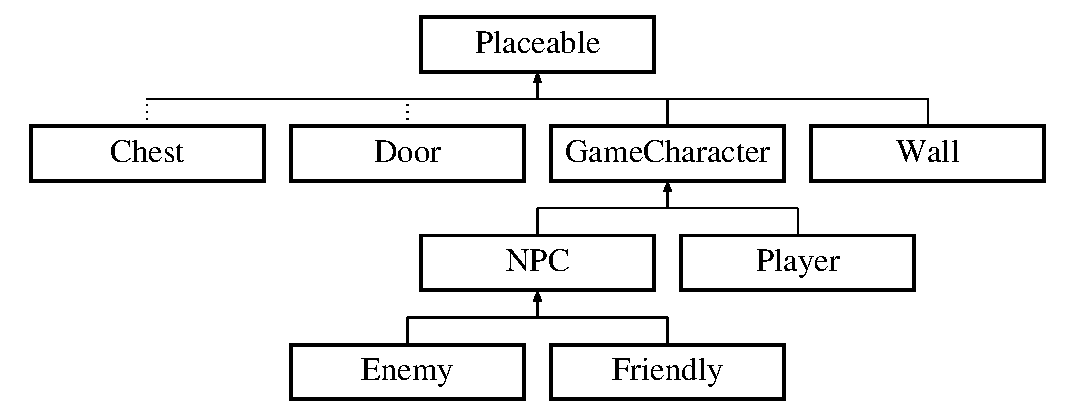
\includegraphics[height=4.000000cm]{class_placeable}
\end{center}
\end{figure}
\subsection*{Public Member Functions}
\begin{DoxyCompactItemize}
\item 
\hypertarget{class_placeable_ac044b1aa2e26da04892ca79ab1082e75}{}\label{class_placeable_ac044b1aa2e26da04892ca79ab1082e75} 
virtual bool {\bfseries is\+Walkable} ()=0
\item 
\hypertarget{class_placeable_afbea2399c9d303b4b0d339cbb85e438b}{}\label{class_placeable_afbea2399c9d303b4b0d339cbb85e438b} 
virtual std\+::string {\bfseries get\+Class\+Name} ()
\item 
\hypertarget{class_placeable_a59b01c6e15b33025d4c46c475654178b}{}\label{class_placeable_a59b01c6e15b33025d4c46c475654178b} 
virtual const char {\bfseries get\+Symbol} ()=0
\item 
\hypertarget{class_placeable_a415577ef15fc368e9d340d2bc3c01bec}{}\label{class_placeable_a415577ef15fc368e9d340d2bc3c01bec} 
virtual void {\bfseries update\+Lvl} (int a\+Level)=0
\item 
\hypertarget{class_placeable_ae1161133792a3fe4d5f5bc60cfbc3a3f}{}\label{class_placeable_ae1161133792a3fe4d5f5bc60cfbc3a3f} 
virtual bool {\bfseries reset} ()=0
\end{DoxyCompactItemize}
\subsection*{Friends}
\begin{DoxyCompactItemize}
\item 
\hypertarget{class_placeable_ac98d07dd8f7b70e16ccb9a01abf56b9c}{}\label{class_placeable_ac98d07dd8f7b70e16ccb9a01abf56b9c} 
class {\bfseries boost\+::serialization\+::access}
\end{DoxyCompactItemize}


\subsection{Detailed Description}


Definition at line 13 of file placeable.\+h.



The documentation for this class was generated from the following file\+:\begin{DoxyCompactItemize}
\item 
placeable.\+h\end{DoxyCompactItemize}

\hypertarget{class_player}{}\section{Player Class Reference}
\label{class_player}\index{Player@{Player}}
Inheritance diagram for Player\+:\begin{figure}[H]
\begin{center}
\leavevmode
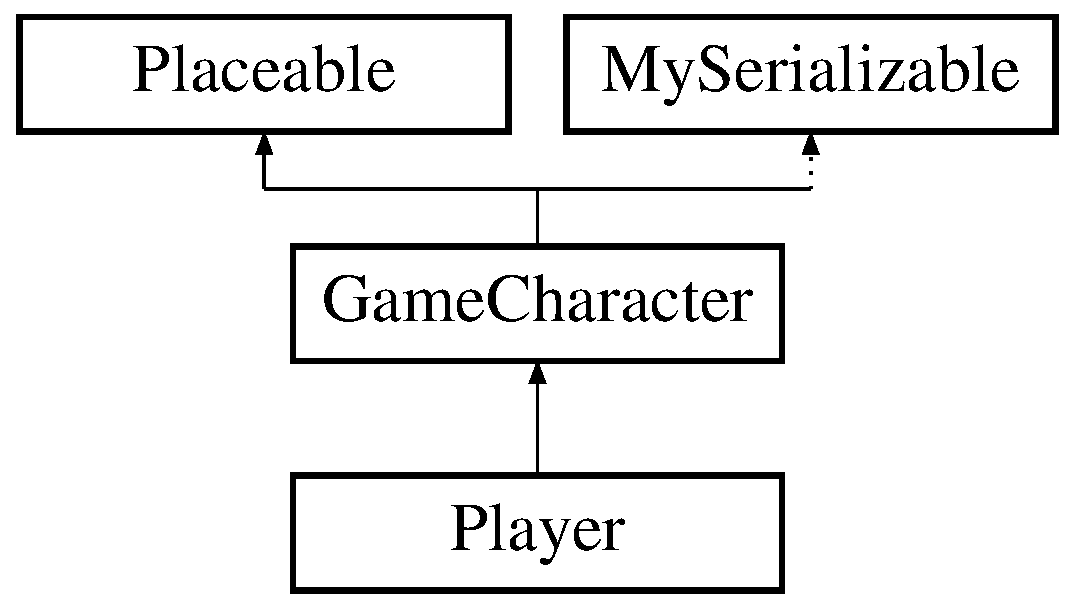
\includegraphics[height=3.000000cm]{class_player}
\end{center}
\end{figure}
\subsection*{Public Member Functions}
\begin{DoxyCompactItemize}
\item 
\hypertarget{class_player_a8caaecc11d0c3ce25fa13c35f01133b6}{}\label{class_player_a8caaecc11d0c3ce25fa13c35f01133b6} 
{\bfseries Player} (std\+::string a\+Name, int a\+Level)
\item 
\hypertarget{class_player_a219f7853f0085cf37af6f500862eb19b}{}\label{class_player_a219f7853f0085cf37af6f500862eb19b} 
const char {\bfseries get\+Symbol} ()
\item 
\hypertarget{class_player_a4971158246dd9cda8ff8140440eac557}{}\label{class_player_a4971158246dd9cda8ff8140440eac557} 
bool {\bfseries is\+Walkable} ()
\item 
\hypertarget{class_player_a588612b72b0e74ba964662ce96e840f2}{}\label{class_player_a588612b72b0e74ba964662ce96e840f2} 
bool {\bfseries reset} ()
\item 
\hypertarget{class_player_ace997edd6d7632c0e28afa5efd5a2174}{}\label{class_player_ace997edd6d7632c0e28afa5efd5a2174} 
void {\bfseries load} (std\+::string filename)
\item 
\hypertarget{class_player_a4d5408ebb2f233bc2157f1e213861369}{}\label{class_player_a4d5408ebb2f233bc2157f1e213861369} 
void {\bfseries save} (std\+::string filename)
\end{DoxyCompactItemize}
\subsection*{Static Public Member Functions}
\begin{DoxyCompactItemize}
\item 
\hypertarget{class_player_ade7d529c6dd53d80e003c94a558ae6b1}{}\label{class_player_ade7d529c6dd53d80e003c94a558ae6b1} 
static \hyperlink{class_player}{Player} {\bfseries s\+Load} (std\+::string filename)
\end{DoxyCompactItemize}
\subsection*{Friends}
\begin{DoxyCompactItemize}
\item 
\hypertarget{class_player_ac98d07dd8f7b70e16ccb9a01abf56b9c}{}\label{class_player_ac98d07dd8f7b70e16ccb9a01abf56b9c} 
class {\bfseries boost\+::serialization\+::access}
\end{DoxyCompactItemize}


\subsection{Detailed Description}


Definition at line 107 of file character.\+h.



The documentation for this class was generated from the following files\+:\begin{DoxyCompactItemize}
\item 
character.\+h\item 
character.\+cpp\end{DoxyCompactItemize}

\hypertarget{class_ring}{}\section{Ring Class Reference}
\label{class_ring}\index{Ring@{Ring}}
Inheritance diagram for Ring\+:\begin{figure}[H]
\begin{center}
\leavevmode
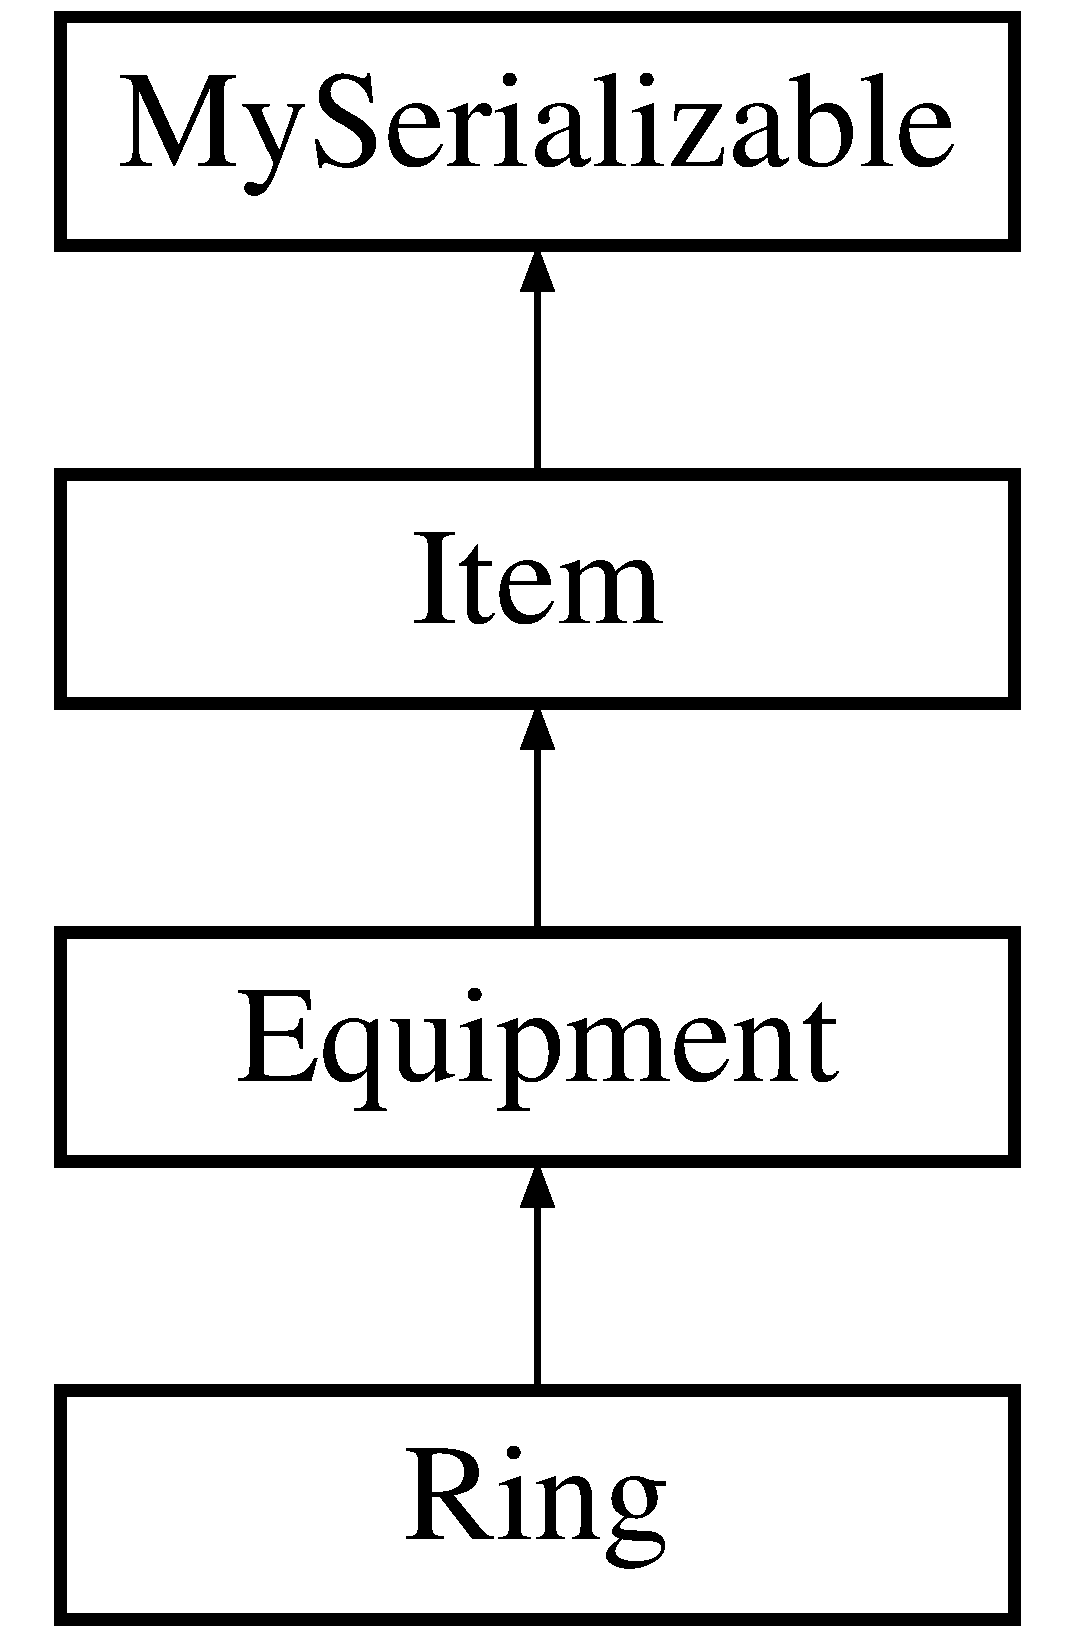
\includegraphics[height=4.000000cm]{class_ring}
\end{center}
\end{figure}
\subsection*{Public Member Functions}
\begin{DoxyCompactItemize}
\item 
\hypertarget{class_ring_a7c6122977579015e8c065663fbda65af}{}\label{class_ring_a7c6122977579015e8c065663fbda65af} 
{\bfseries Ring} (std\+::string a\+Name)
\item 
\hypertarget{class_ring_a0191f59fb68ddf34ebcb99e3f24ab494}{}\label{class_ring_a0191f59fb68ddf34ebcb99e3f24ab494} 
\hyperlink{class_equip_type}{Equip\+Type} const  $\ast$ {\bfseries get\+Type} ()
\item 
\hypertarget{class_ring_aff7a3645b12cf93682ffbf36a7e4cc12}{}\label{class_ring_aff7a3645b12cf93682ffbf36a7e4cc12} 
virtual void {\bfseries save} (std\+::string filename)
\item 
\hypertarget{class_ring_abf9eadeb142d0e70fe1d6caeded4fa90}{}\label{class_ring_abf9eadeb142d0e70fe1d6caeded4fa90} 
virtual void {\bfseries load} (std\+::string filename)
\end{DoxyCompactItemize}
\subsection*{Static Public Member Functions}
\begin{DoxyCompactItemize}
\item 
\hypertarget{class_ring_a57af1c46d6d51c36dcc2b9eec412132b}{}\label{class_ring_a57af1c46d6d51c36dcc2b9eec412132b} 
static \hyperlink{class_ring}{Ring} {\bfseries s\+Load} (std\+::string filename)
\end{DoxyCompactItemize}
\subsection*{Friends}
\begin{DoxyCompactItemize}
\item 
\hypertarget{class_ring_ac98d07dd8f7b70e16ccb9a01abf56b9c}{}\label{class_ring_ac98d07dd8f7b70e16ccb9a01abf56b9c} 
class {\bfseries boost\+::serialization\+::access}
\end{DoxyCompactItemize}
\subsection*{Additional Inherited Members}


\subsection{Detailed Description}


Definition at line 237 of file inv2.\+h.



The documentation for this class was generated from the following files\+:\begin{DoxyCompactItemize}
\item 
inv2.\+h\item 
inv2.\+cpp\end{DoxyCompactItemize}

\hypertarget{class_shield}{}\section{Shield Class Reference}
\label{class_shield}\index{Shield@{Shield}}
Inheritance diagram for Shield\+:\begin{figure}[H]
\begin{center}
\leavevmode
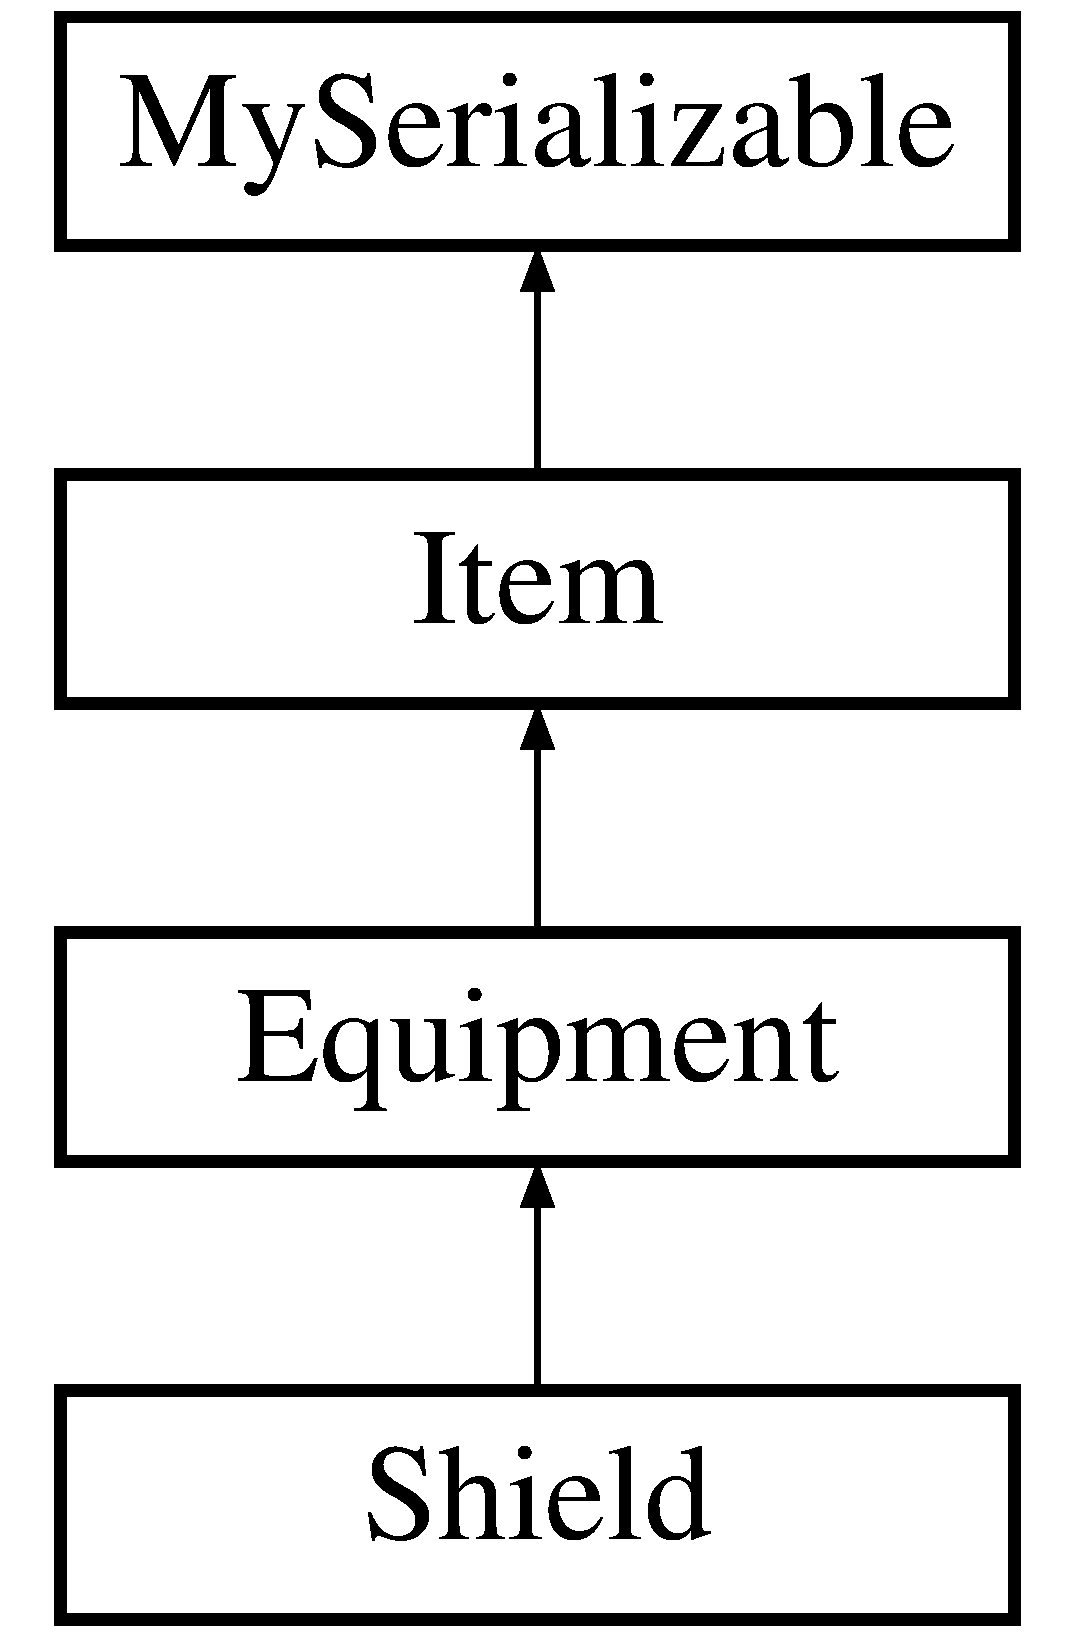
\includegraphics[height=4.000000cm]{class_shield}
\end{center}
\end{figure}
\subsection*{Public Member Functions}
\begin{DoxyCompactItemize}
\item 
\hypertarget{class_shield_a1e9be80b91c5d7014040cb8b0b1be617}{}\label{class_shield_a1e9be80b91c5d7014040cb8b0b1be617} 
{\bfseries Shield} (std\+::string a\+Name)
\item 
\hypertarget{class_shield_a3638b0f119c2a80a35fc5a0a8a1149b7}{}\label{class_shield_a3638b0f119c2a80a35fc5a0a8a1149b7} 
\hyperlink{class_equip_type}{Equip\+Type} const  $\ast$ {\bfseries get\+Type} ()
\item 
\hypertarget{class_shield_acc7d400fb1ec819120f790a9bf85f6e9}{}\label{class_shield_acc7d400fb1ec819120f790a9bf85f6e9} 
virtual void {\bfseries save} (std\+::string filename)
\item 
\hypertarget{class_shield_a8b4e9e3b143f67400d082b2aec8fa430}{}\label{class_shield_a8b4e9e3b143f67400d082b2aec8fa430} 
virtual void {\bfseries load} (std\+::string filename)
\end{DoxyCompactItemize}
\subsection*{Static Public Member Functions}
\begin{DoxyCompactItemize}
\item 
\hypertarget{class_shield_a57f4a10d8516f2fdf6a790c553bcd4e5}{}\label{class_shield_a57f4a10d8516f2fdf6a790c553bcd4e5} 
static \hyperlink{class_shield}{Shield} {\bfseries s\+Load} (std\+::string filename)
\end{DoxyCompactItemize}
\subsection*{Friends}
\begin{DoxyCompactItemize}
\item 
\hypertarget{class_shield_ac98d07dd8f7b70e16ccb9a01abf56b9c}{}\label{class_shield_ac98d07dd8f7b70e16ccb9a01abf56b9c} 
class {\bfseries boost\+::serialization\+::access}
\end{DoxyCompactItemize}
\subsection*{Additional Inherited Members}


\subsection{Detailed Description}


Definition at line 262 of file inv2.\+h.



The documentation for this class was generated from the following files\+:\begin{DoxyCompactItemize}
\item 
inv2.\+h\item 
inv2.\+cpp\end{DoxyCompactItemize}

\hypertarget{class_string_func}{}\section{String\+Func Class Reference}
\label{class_string_func}\index{String\+Func@{String\+Func}}
\subsection*{Static Public Member Functions}
\begin{DoxyCompactItemize}
\item 
\hypertarget{class_string_func_ae4f83e5ac07871e85547dc287bde3ff5}{}\label{class_string_func_ae4f83e5ac07871e85547dc287bde3ff5} 
static string {\bfseries to\+Lower\+Case} (string a\+String)
\end{DoxyCompactItemize}


\subsection{Detailed Description}


Definition at line 116 of file config.\+h.



The documentation for this class was generated from the following file\+:\begin{DoxyCompactItemize}
\item 
config.\+h\end{DoxyCompactItemize}

\hypertarget{class_wall}{}\section{Wall Class Reference}
\label{class_wall}\index{Wall@{Wall}}
Inheritance diagram for Wall\+:\begin{figure}[H]
\begin{center}
\leavevmode
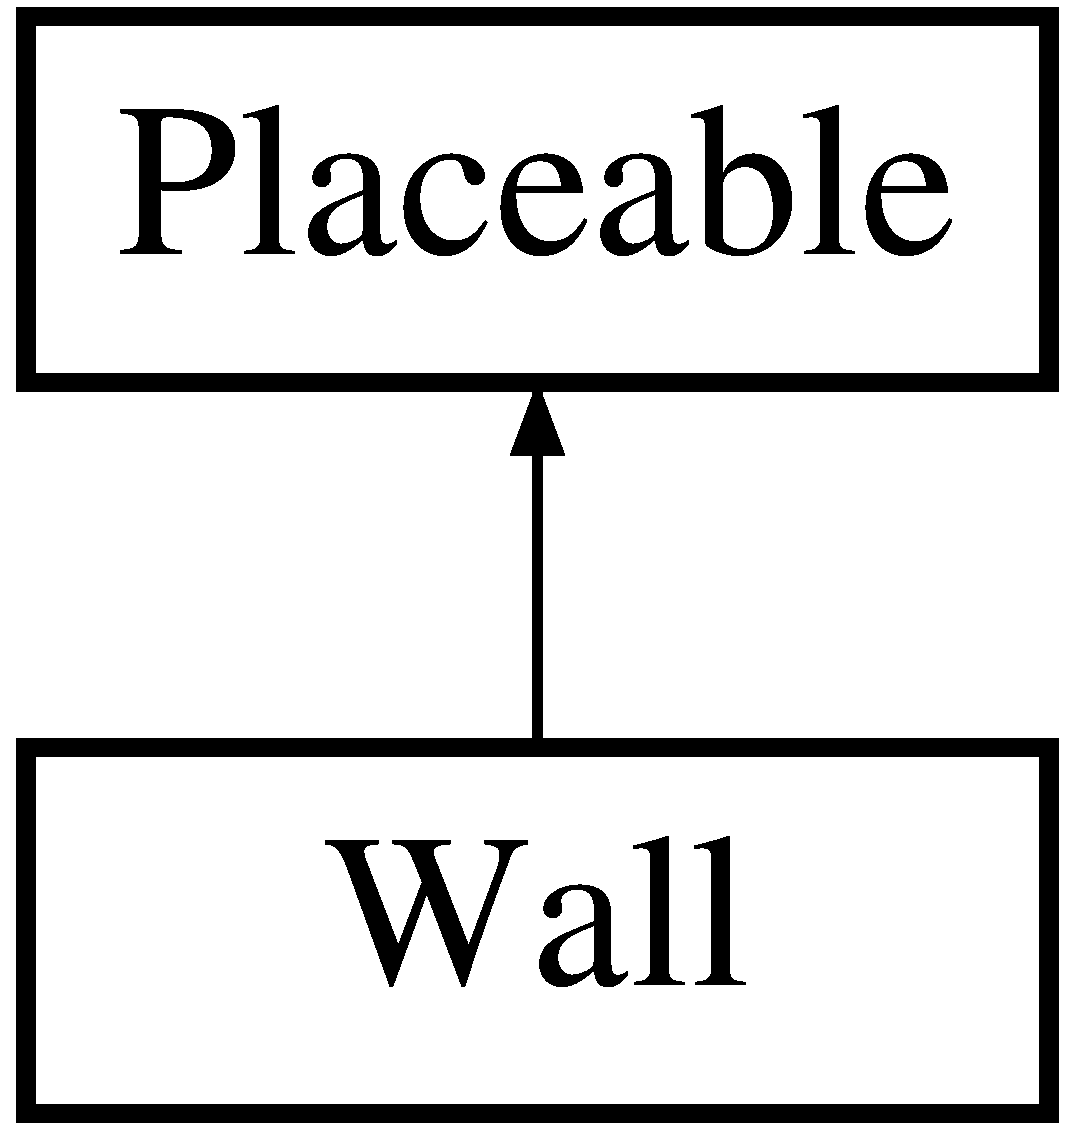
\includegraphics[height=2.000000cm]{class_wall}
\end{center}
\end{figure}
\subsection*{Public Member Functions}
\begin{DoxyCompactItemize}
\item 
\hypertarget{class_wall_a0c87e6f71e807e46721712b75d7fe5ad}{}\label{class_wall_a0c87e6f71e807e46721712b75d7fe5ad} 
const char {\bfseries get\+Symbol} ()
\item 
\hypertarget{class_wall_a115c65e30af750fdf1c74392495bac4c}{}\label{class_wall_a115c65e30af750fdf1c74392495bac4c} 
void {\bfseries update\+Lvl} (int a\+Level)
\item 
\hypertarget{class_wall_ab7b0b368cae9727d00125ba37381206a}{}\label{class_wall_ab7b0b368cae9727d00125ba37381206a} 
bool {\bfseries is\+Walkable} ()
\item 
\hypertarget{class_wall_a6320565e6c2d93e2cc1e2aa400d27401}{}\label{class_wall_a6320565e6c2d93e2cc1e2aa400d27401} 
bool {\bfseries reset} ()
\end{DoxyCompactItemize}
\subsection*{Friends}
\begin{DoxyCompactItemize}
\item 
\hypertarget{class_wall_ac98d07dd8f7b70e16ccb9a01abf56b9c}{}\label{class_wall_ac98d07dd8f7b70e16ccb9a01abf56b9c} 
class {\bfseries boost\+::serialization\+::access}
\end{DoxyCompactItemize}


\subsection{Detailed Description}


Definition at line 40 of file basic\+\_\+structure.\+h.



The documentation for this class was generated from the following file\+:\begin{DoxyCompactItemize}
\item 
basic\+\_\+structure.\+h\end{DoxyCompactItemize}

\hypertarget{class_weapon}{}\section{Weapon Class Reference}
\label{class_weapon}\index{Weapon@{Weapon}}
Inheritance diagram for Weapon\+:\begin{figure}[H]
\begin{center}
\leavevmode
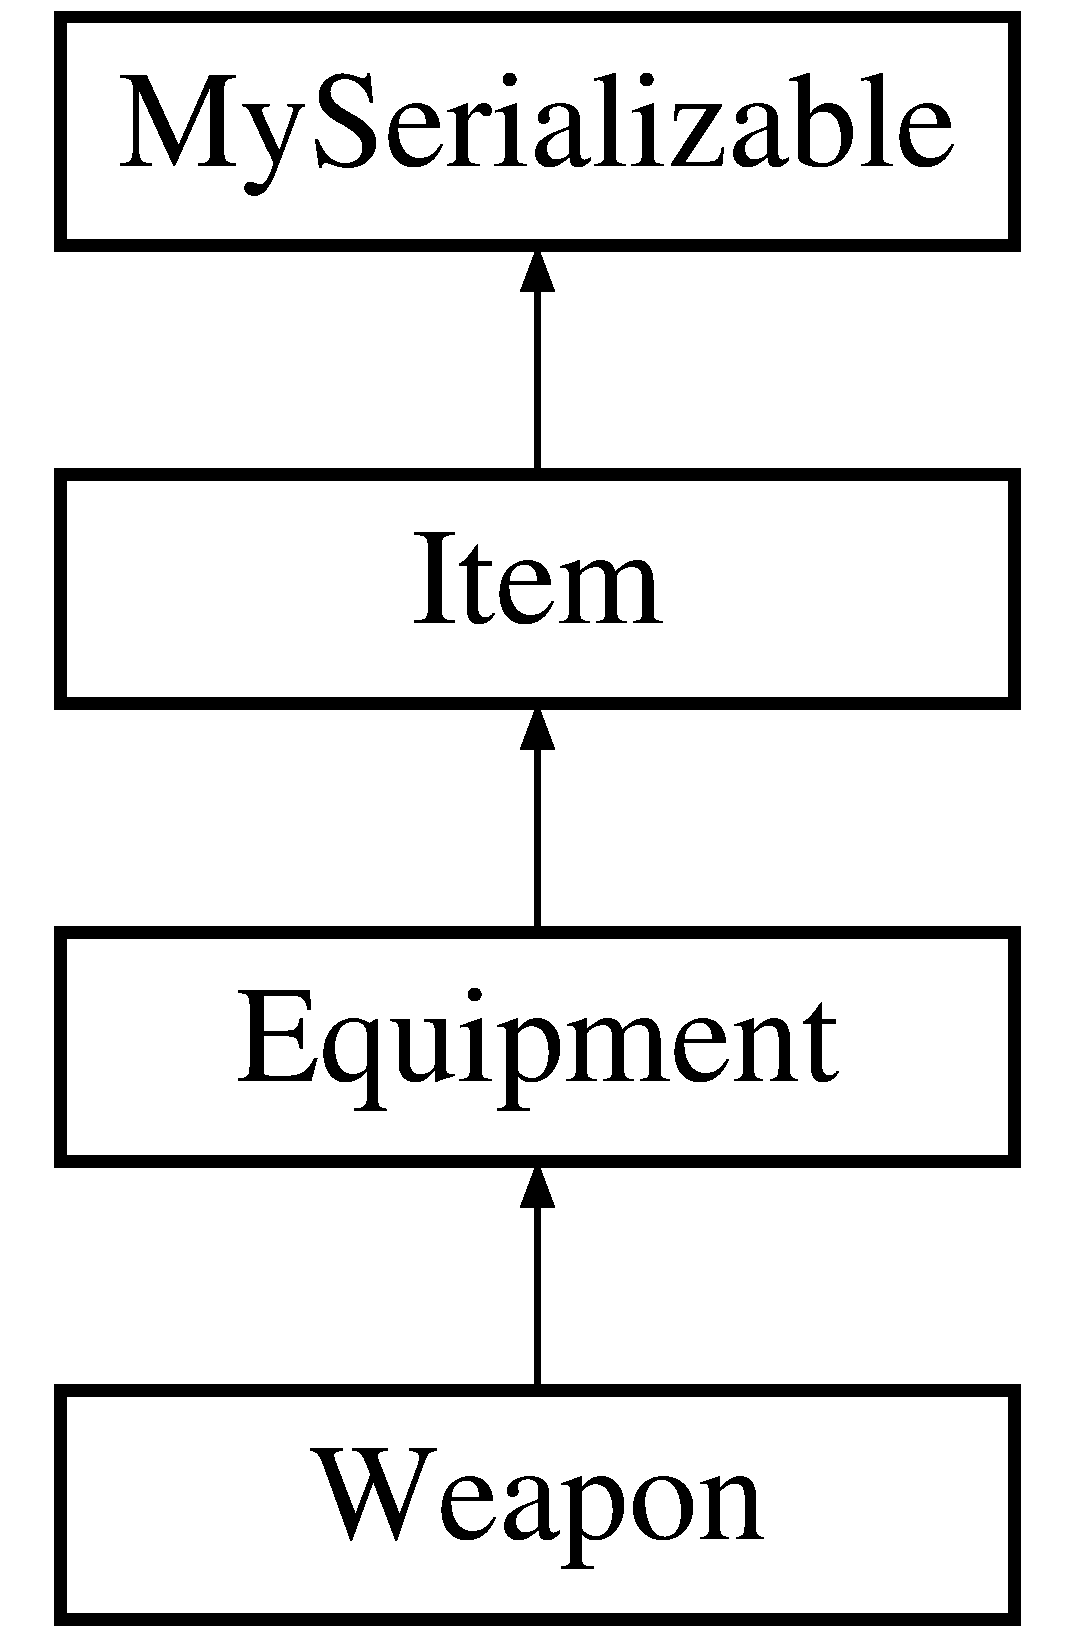
\includegraphics[height=4.000000cm]{class_weapon}
\end{center}
\end{figure}
\subsection*{Public Member Functions}
\begin{DoxyCompactItemize}
\item 
\hypertarget{class_weapon_ad0708441316f06924b0da0c288b99136}{}\label{class_weapon_ad0708441316f06924b0da0c288b99136} 
{\bfseries Weapon} (std\+::string a\+Name)
\item 
\hypertarget{class_weapon_a6b9a83e88b0d07a52ac605bd0044b26a}{}\label{class_weapon_a6b9a83e88b0d07a52ac605bd0044b26a} 
virtual \hyperlink{class_equip_type}{Equip\+Type} const  $\ast$ {\bfseries get\+Type} ()
\item 
\hypertarget{class_weapon_a2014e6757365a58d5d7815a717903347}{}\label{class_weapon_a2014e6757365a58d5d7815a717903347} 
void {\bfseries set\+Range} (int new\+Range)
\item 
\hypertarget{class_weapon_af0d86939f16add54fc7ae87fea85ac21}{}\label{class_weapon_af0d86939f16add54fc7ae87fea85ac21} 
int {\bfseries get\+Range} ()
\item 
\hypertarget{class_weapon_a226746903ddaa7abb177665abd597086}{}\label{class_weapon_a226746903ddaa7abb177665abd597086} 
int {\bfseries get\+Base\+Attk} ()
\item 
\hypertarget{class_weapon_ab23a119713f3e433f0d3e90659ab435d}{}\label{class_weapon_ab23a119713f3e433f0d3e90659ab435d} 
void {\bfseries set\+Base\+Attk} (int value)
\item 
\hypertarget{class_weapon_ae382102dd74948449b7eadbb2f24bc06}{}\label{class_weapon_ae382102dd74948449b7eadbb2f24bc06} 
virtual void {\bfseries save} (std\+::string filename)
\item 
\hypertarget{class_weapon_a541515ce9e8394c01473dd4282cc1dfe}{}\label{class_weapon_a541515ce9e8394c01473dd4282cc1dfe} 
virtual void {\bfseries load} (std\+::string filename)
\end{DoxyCompactItemize}
\subsection*{Static Public Member Functions}
\begin{DoxyCompactItemize}
\item 
\hypertarget{class_weapon_a4dd598f04fed0db98db6e4d4a3cd8e23}{}\label{class_weapon_a4dd598f04fed0db98db6e4d4a3cd8e23} 
static \hyperlink{class_weapon}{Weapon} {\bfseries s\+Load} (std\+::string filename)
\end{DoxyCompactItemize}
\subsection*{Friends}
\begin{DoxyCompactItemize}
\item 
\hypertarget{class_weapon_ac98d07dd8f7b70e16ccb9a01abf56b9c}{}\label{class_weapon_ac98d07dd8f7b70e16ccb9a01abf56b9c} 
class {\bfseries boost\+::serialization\+::access}
\end{DoxyCompactItemize}
\subsection*{Additional Inherited Members}


\subsection{Detailed Description}


Definition at line 279 of file inv2.\+h.



The documentation for this class was generated from the following files\+:\begin{DoxyCompactItemize}
\item 
inv2.\+h\item 
inv2.\+cpp\end{DoxyCompactItemize}

%--- End generated contents ---

% Index
\backmatter
\newpage
\phantomsection
\clearemptydoublepage
\addcontentsline{toc}{chapter}{Index}
\printindex

\end{document}
